% power_diode_fundamentals_it.tex
% Fondamenti di dispositivi a semiconduttore: il diodo di potenza.
% Versione italiana; la versione inglese è power_diode_fundamentals.tex (stessa struttura, stesse etichette, stesse equazioni).
% Documento unico che raccoglie e armonizza tre note di questa cartella (research/power_semiconductor_devices/diode):
%   power_diode/power_diode.tex                        struttura PIN, bande, conduzione, reverse recovery, tecnologie
%   charge_control_model/charge_control.tex            equazione ambipolare e modello a controllo di carica
%   lauritzen_ma_datasheet_conversion/..._it.tex       modello di Lauritzen-Ma e conversione dei dati del datasheet
% Le tre note restano al loro posto; l'Appendice C elenca la corrispondenza dei simboli e ciò che è stato corretto.
% Template pwr-control (AAA_template_latex_settings). Numeri e figure:
%   power_diode_fundamentals_calc.py  ->  power_diode_fundamentals_values.tex (macro \pd...), figures/fig_*_it.pdf
%   ../lauritzen_ma_datasheet_conversion/lm_conversion_calc.py  ->  lm_conversion_values.tex (macro \lm...),
%   figures/fig_*_it.pdf di quella cartella: questo documento li legge da lì, senza copiarli
% Compilazione, da questa cartella: pdflatex power_diode_fundamentals_it.tex  (tre volte, per indice e riferimenti)
% Rev. 00 - novembre 2026 - prima emissione
\documentclass[10pt,a4paper]{scrartcl}
\PassOptionsToPackage{main=italian}{babel}   % settings.tex carica babel con [british]: l'italiano diventa la lingua principale
\input{../../../../AAA_template_latex_settings/settings}
% il documento sta quattro livelli sotto la radice del repository: percorso del logo di settings.tex corretto qui
\rhead{\includegraphics[height=0.75cm]{../../../../AAA_template_latex_settings/pwr-control_logo_doc.png}}
\rfoot{\small Rev.~00}
\geometry{left=2.0cm, right=2.0cm}\setlength{\headwidth}{\textwidth}
\usepackage[european resistors, american inductors]{circuitikz}
\usetikzlibrary{patterns}
\usepackage[T1]{fontenc}\usepackage{lmodern}\usepackage{icomma}   % T1 e Latin Modern: nel PDF lettere accentate e underscore sono caratteri veri (ricerca e copia del testo) e nessun font è bitmap; icomma: virgola decimale nelle formule, 0,35 senza lo spazio della punteggiatura
\babelhyphenation[italian]{data-sheet soft-ness life-time char-ac-ter-is-tics}   % prestiti inglesi

\sisetup{output-decimal-marker={,},per-mode=symbol,range-phrase={\text{--}},range-units=single}
\setlist{nosep}
\setlength{\parindent}{0pt}
\setlength{\parskip}{3pt}
\allowdisplaybreaks
\widowpenalty=10000 \clubpenalty=10000 \makeatletter\@clubpenalty=\clubpenalty\makeatother \displaywidowpenalty=10000 \makeatletter\addto\extrasitalian{\widowpenalty=10000 \clubpenalty=10000 \@clubpenalty=\clubpenalty}\makeatother   % nessuna riga isolata in cima o in fondo a una pagina, né prima di una formula; \addto\extrasitalian perché babel-italian, all'inizio del documento, riporta a 3000 le prime due penalità
\captionsetup{font=small,labelfont=bf}
\RedeclareSectionCommand[tocnumwidth=2.2em]{section}   % indice: spazio per i numeri di sezione a due cifre
\RedeclareSectionCommand[tocindent=2.2em,tocnumwidth=3.0em]{subsection}
\renewcommand{\topfraction}{0.9}
\renewcommand{\bottomfraction}{0.9}
\renewcommand{\textfraction}{0.05}
\renewcommand{\floatpagefraction}{0.8}

% --- numeri (generati dai due script) ---
% I due file di valori sono letti sostituendo il punto decimale con la virgola: ogni macro \pd... o \lm...
% si espande in un numero come 1,879, valido sia nel testo sia dentro \SI{}{} e \num{} di siunitx.
\ExplSyntaxOn
\cs_new_protected:Npn \pdvaluedefine #1#2
  {
    \tl_set:Nn \l_tmpa_tl {#2}
    \tl_replace_all:Nnn \l_tmpa_tl { . } { , }
    \cs_gset_eq:NN #1 \l_tmpa_tl
  }
\ExplSyntaxOff
\begingroup
\let\newcommand\pdvaluedefine
% generated by power_diode_fundamentals_calc.py: do not edit by hand
\newcommand{\pdVt}{25.85}
\newcommand{\pdMun}{1400}
\newcommand{\pdMup}{450}
\newcommand{\pdMusum}{1850}
\newcommand{\pdDn}{36}
\newcommand{\pdDp}{12}
\newcommand{\pdDa}{18}
\newcommand{\pdDaOne}{17.6}
\newcommand{\pdBratio}{3.1}
\newcommand{\pdBmob}{0.51}
\newcommand{\pdOneMinusBsq}{0.74}
\newcommand{\pdSigmaRatio}{1.32}
\newcommand{\pdEpsR}{11.7}
\newcommand{\pdEpsFcm}{1.04}
\newcommand{\pdLaOne}{42}
\newcommand{\pdLaTen}{133}
\newcommand{\pdVmAsymCoef}{1.35}
\newcommand{\pdVmHandCoef}{1.18}
\newcommand{\pdThreePiEight}{1.18}
\newcommand{\pdDaHotA}{12}
\newcommand{\pdDaHotB}{11}
\newcommand{\pdNiDoubleLo}{8}
\newcommand{\pdNiDoubleHi}{15}
\newcommand{\pdNiRatio}{540}
\newcommand{\pdEgZero}{1.2}
\newcommand{\pdTcVjLo}{0.60}
\newcommand{\pdTcLo}{2.3}
\newcommand{\pdTcVjHi}{0.82}
\newcommand{\pdTcHi}{1.5}
\newcommand{\pdTauAugerLo}{263}
\newcommand{\pdTauAugerHi}{2.6}
\newcommand{\pdBlkNdA}{2\times10^{13}}
\newcommand{\pdBlkEcA}{1.84}
\newcommand{\pdBlkVA}{5500}
\newcommand{\pdBlkWA}{596}
\newcommand{\pdBlkRA}{13.29}
\newcommand{\pdBlkDropA}{1329}
\newcommand{\pdBlkNdB}{5\times10^{13}}
\newcommand{\pdBlkEcB}{2.07}
\newcommand{\pdBlkVB}{2760}
\newcommand{\pdBlkWB}{267}
\newcommand{\pdBlkRB}{2.38}
\newcommand{\pdBlkDropB}{238}
\newcommand{\pdBlkNdC}{1\times10^{14}}
\newcommand{\pdBlkEcC}{2.25}
\newcommand{\pdBlkVC}{1640}
\newcommand{\pdBlkWC}{146}
\newcommand{\pdBlkRC}{0.65}
\newcommand{\pdBlkDropC}{65}
\newcommand{\pdBlkNdD}{2\times10^{14}}
\newcommand{\pdBlkEcD}{2.46}
\newcommand{\pdBlkVD}{980}
\newcommand{\pdBlkWD}{80}
\newcommand{\pdBlkRD}{0.18}
\newcommand{\pdBlkDropD}{18}
\newcommand{\pdBlkCoefV}{5.2\times10^{13}}
\newcommand{\pdBlkCoefW}{2.6\times10^{10}}
\newcommand{\pdTgtV}{2}
\newcommand{\pdTgtNd}{7.7\times10^{13}}
\newcommand{\pdTgtW}{183}
\newcommand{\pdTgtR}{1.1}
\newcommand{\pdTgtDrop}{110}
\newcommand{\pdPtNd}{3\times10^{13}}
\newcommand{\pdPtW}{120}
\newcommand{\pdPtSavePct}{34}
\newcommand{\pdPtEc}{1.94}
\newcommand{\pdExVbr}{1480}
\newcommand{\pdDynPLo}{6.2\times10^{13}}
\newcommand{\pdDynPctLo}{62}
\newcommand{\pdDynJLo}{100}
\newcommand{\pdDynVbrLo}{1140}
\newcommand{\pdDynPHi}{1.9\times10^{14}}
\newcommand{\pdDynPctHi}{187}
\newcommand{\pdDynJHi}{300}
\newcommand{\pdDynVbrHi}{750}
\newcommand{\pdVbi}{0.77}
\newcommand{\pdVbiTwo}{0.30}
\newcommand{\pdScV}{600}
\newcommand{\pdScWZero}{3.2}
\newcommand{\pdScW}{88}
\newcommand{\pdScCjZero}{3.3}
\newcommand{\pdScCj}{120}
\newcommand{\pdScQc}{0.14}
\newcommand{\pdExVrt}{770}
\newcommand{\pdScQcPct}{0.14}
\newcommand{\pdJgenUa}{14}
\newcommand{\pdExW}{100}
\newcommand{\pdExNd}{1\times10^{14}}
\newcommand{\pdExJ}{100}
\newcommand{\pdExRuni}{0.45}
\newcommand{\pdExDropUni}{45}
\newcommand{\pdExNa}{1\times10^{19}}
\newcommand{\pdHem}{2\times10^{-14}}
\newcommand{\pdExRho}{45}
\newcommand{\pdLpOne}{34}
\newcommand{\pdJsShockley}{5.5\times10^{-10}}
\newcommand{\pdHiOnsetV}{0.48}
\newcommand{\pdHiOnsetJ}{50}
\newcommand{\pdExSlowTau}{10}
\newcommand{\pdExSlowLa}{133}
\newcommand{\pdExSlowBeta}{0.38}
\newcommand{\pdExSlowPbar}{6.2\times10^{17}}
\newcommand{\pdExSlowPl}{7.0\times10^{17}}
\newcommand{\pdExSlowPr}{6.1\times10^{17}}
\newcommand{\pdExSlowPmin}{6.0\times10^{17}}
\newcommand{\pdExSlowQs}{1000}
\newcommand{\pdExSlowSigRatio}{8250}
\newcommand{\pdExSlowVmFlat}{5}
\newcommand{\pdExSlowVm}{7}
\newcommand{\pdExSlowVmOhm}{5}
\newcommand{\pdExSlowVmDem}{2}
\newcommand{\pdExSlowVmThin}{7}
\newcommand{\pdExSlowVjOne}{0.70}
\newcommand{\pdExSlowVjTwo}{0.23}
\newcommand{\pdExSlowVf}{0.94}
\newcommand{\pdExSlowTmStat}{0.05}
\newcommand{\pdExSlowEmQs}{171}
\newcommand{\pdExSlowEmTauEff}{1.71}
\newcommand{\pdExSlowEmTauPct}{17}
\newcommand{\pdExSlowEmPct}{83}
\newcommand{\pdExSlowEmVf}{0.88}
\newcommand{\pdExSlowEmVm}{37}
\newcommand{\pdExSlowEmPl}{1.3\times10^{17}}
\newcommand{\pdExSlowEmPr}{9.2\times10^{16}}
\newcommand{\pdExSlowEmPbar}{1.1\times10^{17}}
\newcommand{\pdExSlowEmSlopeVj}{1.07}
\newcommand{\pdExSlowEmSlopeVf}{1.67}
\newcommand{\pdExSlowQflOne}{0.93}
\newcommand{\pdExSlowTauAuger}{7}
\newcommand{\pdExMidTau}{1}
\newcommand{\pdExMidLa}{42}
\newcommand{\pdExMidBeta}{1.19}
\newcommand{\pdExMidPbar}{6.2\times10^{16}}
\newcommand{\pdExMidPl}{1.2\times10^{17}}
\newcommand{\pdExMidPr}{5.8\times10^{16}}
\newcommand{\pdExMidPmin}{4.5\times10^{16}}
\newcommand{\pdExMidQs}{100}
\newcommand{\pdExMidSigRatio}{820}
\newcommand{\pdExMidVmFlat}{54}
\newcommand{\pdExMidVm}{69}
\newcommand{\pdExMidVmOhm}{59}
\newcommand{\pdExMidVmDem}{10}
\newcommand{\pdExMidVmThin}{73}
\newcommand{\pdExMidVjOne}{0.66}
\newcommand{\pdExMidVjTwo}{0.16}
\newcommand{\pdExMidVf}{0.89}
\newcommand{\pdExMidTmStat}{0.43}
\newcommand{\pdExMidEmQs}{71}
\newcommand{\pdExMidEmTauEff}{0.71}
\newcommand{\pdExMidEmTauPct}{71}
\newcommand{\pdExMidEmPct}{29}
\newcommand{\pdExMidEmVf}{0.90}
\newcommand{\pdExMidEmVm}{91}
\newcommand{\pdExMidEmPl}{8.5\times10^{16}}
\newcommand{\pdExMidEmPr}{4.3\times10^{16}}
\newcommand{\pdExMidEmPbar}{4.4\times10^{16}}
\newcommand{\pdExMidEmSlopeVj}{1.57}
\newcommand{\pdExMidEmSlopeVf}{2.24}
\newcommand{\pdExMidQflOne}{0.84}
\newcommand{\pdExMidTauAuger}{676}
\newcommand{\pdExFastTau}{0.3}
\newcommand{\pdExFastLa}{23}
\newcommand{\pdExFastBeta}{2.18}
\newcommand{\pdExFastPbar}{1.9\times10^{16}}
\newcommand{\pdExFastPl}{6.2\times10^{16}}
\newcommand{\pdExFastPr}{2.1\times10^{16}}
\newcommand{\pdExFastPmin}{8.1\times10^{15}}
\newcommand{\pdExFastQs}{30}
\newcommand{\pdExFastSigRatio}{250}
\newcommand{\pdExFastVmFlat}{180}
\newcommand{\pdExFastVm}{265}
\newcommand{\pdExFastVmOhm}{251}
\newcommand{\pdExFastVmDem}{14}
\newcommand{\pdExFastVmThin}{245}
\newcommand{\pdExFastVjOne}{0.64}
\newcommand{\pdExFastVjTwo}{0.14}
\newcommand{\pdExFastVf}{1.05}
\newcommand{\pdExFastTmStat}{1.23}
\newcommand{\pdExFastEmQs}{27}
\newcommand{\pdExFastEmTauEff}{0.27}
\newcommand{\pdExFastEmTauPct}{89}
\newcommand{\pdExFastEmPct}{11}
\newcommand{\pdExFastEmVf}{1.07}
\newcommand{\pdExFastEmVm}{290}
\newcommand{\pdExFastEmPl}{5.4\times10^{16}}
\newcommand{\pdExFastEmPr}{2.0\times10^{16}}
\newcommand{\pdExFastEmPbar}{1.7\times10^{16}}
\newcommand{\pdExFastEmSlopeVj}{1.83}
\newcommand{\pdExFastEmSlopeVf}{2.71}
\newcommand{\pdExFastQflOne}{0.81}
\newcommand{\pdExFastTauAuger}{7506}
\newcommand{\pdVmHalfVt}{0.48}
\newcommand{\pdVmHalfMv}{12}
\newcommand{\pdVmThinErrHalfPct}{3}
\newcommand{\pdVmAsymErrHalfPct}{360}
\newcommand{\pdVmHandErrHalfPct}{302}
\newcommand{\pdVmThinSgnHalf}{+3}
\newcommand{\pdVmAsymSgnHalf}{+360}
\newcommand{\pdVmHandSgnHalf}{+302}
\newcommand{\pdVmFlatLowHalfPct}{24}
\newcommand{\pdVmOneVt}{1.87}
\newcommand{\pdVmOneMv}{48}
\newcommand{\pdVmThinErrOnePct}{7}
\newcommand{\pdVmAsymErrOnePct}{96}
\newcommand{\pdVmHandErrOnePct}{72}
\newcommand{\pdVmThinSgnOne}{+7}
\newcommand{\pdVmAsymSgnOne}{+96}
\newcommand{\pdVmHandSgnOne}{+72}
\newcommand{\pdVmFlatLowOnePct}{21}
\newcommand{\pdVmTwoVt}{8.30}
\newcommand{\pdVmTwoMv}{215}
\newcommand{\pdVmThinErrTwoPct}{4}
\newcommand{\pdVmAsymErrTwoPct}{20}
\newcommand{\pdVmHandErrTwoPct}{5}
\newcommand{\pdVmThinSgnTwo}{-4}
\newcommand{\pdVmAsymSgnTwo}{+20}
\newcommand{\pdVmHandSgnTwo}{+5}
\newcommand{\pdVmFlatLowTwoPct}{29}
\newcommand{\pdVmThreeVt}{25.5}
\newcommand{\pdVmThreeMv}{661}
\newcommand{\pdVmThinErrThreePct}{30}
\newcommand{\pdVmAsymErrThreePct}{6}
\newcommand{\pdVmHandErrThreePct}{7}
\newcommand{\pdVmThinSgnThree}{-30}
\newcommand{\pdVmAsymSgnThree}{+6}
\newcommand{\pdVmHandSgnThree}{-7}
\newcommand{\pdVmFlatLowThreePct}{48}
\newcommand{\pdVmFourVt}{72.1}
\newcommand{\pdVmFourMv}{1865}
\newcommand{\pdVmThinErrFourPct}{56}
\newcommand{\pdVmAsymErrFourPct}{2}
\newcommand{\pdVmHandErrFourPct}{11}
\newcommand{\pdVmThinSgnFour}{-56}
\newcommand{\pdVmAsymSgnFour}{+2}
\newcommand{\pdVmHandSgnFour}{-11}
\newcommand{\pdVmFlatLowFourPct}{67}
\newcommand{\pdVmFlatLowPct}{26}
\newcommand{\pdDemberLimit}{0.58}
\newcommand{\pdVfMinBeta}{0.95}
\newcommand{\pdVfMinTau}{1.6}
\newcommand{\pdVfMin}{0.89}
\newcommand{\pdVfFlatLo}{0.7}
\newcommand{\pdVfFlatHi}{1.3}
\newcommand{\pdExMidSigma}{18}
\newcommand{\pdRelaxFs}{60}
\newcommand{\pdDebyeNm}{12}
\newcommand{\pdRelaxPs}{50}
\newcommand{\pdExTmPar}{470}
\newcommand{\pdExTmMode}{580}
\newcommand{\pdEmJLo}{10}
\newcommand{\pdEmJLoTauEff}{0.95}
\newcommand{\pdEmJLoPct}{5}
\newcommand{\pdEmJMid}{100}
\newcommand{\pdEmJMidTauEff}{0.71}
\newcommand{\pdEmJMidPct}{29}
\newcommand{\pdEmJHi}{300}
\newcommand{\pdEmJHiTauEff}{0.53}
\newcommand{\pdEmJHiPct}{47}
\newcommand{\pdTsOne}{0.69}
\newcommand{\pdTsFour}{1.61}
\newcommand{\pdRampFracFast}{91}
\newcommand{\pdRampLamFast}{0.2}
\newcommand{\pdRampFracMid}{63}
\newcommand{\pdRampLamMid}{1.0}
\newcommand{\pdRampFracSlow}{20}
\newcommand{\pdRampLamSlow}{5.0}
\newcommand{\pdRampYFast}{0.51}
\newcommand{\pdRampQrrFast}{64}
\newcommand{\pdRampIrrIfFast}{2.53}
\newcommand{\pdRampYMid}{0.84}
\newcommand{\pdRampQrrMid}{35}
\newcommand{\pdRampIrrIfMid}{0.84}
\newcommand{\pdRampYSlow}{1.00}
\newcommand{\pdRampQrrSlow}{10}
\newcommand{\pdRampIrrIfSlow}{0.20}
\newcommand{\pdTmModeRatioPct}{22}
\newcommand{\pdTmAsymFactor}{2.5}
\newcommand{\pdDistTaQuarter}{0.95}
\newcommand{\pdDistTmQuarter}{0.051}
\newcommand{\pdDistTmGeomQuarter}{2.47}
\newcommand{\pdDistSQuarter}{0.10}
\newcommand{\pdDistTauFitQuarter}{1.00}
\newcommand{\pdDistTmFitQuarter}{0.051}
\newcommand{\pdDistWidthQuarter}{1.56}
\newcommand{\pdTmPeakPosQuarter}{0.50}
\newcommand{\pdTmBlockSymQuarter}{0.99}
\newcommand{\pdTmBlockAsymQuarter}{2.5}
\newcommand{\pdDistTaHalf}{0.84}
\newcommand{\pdDistTmHalf}{0.189}
\newcommand{\pdDistTmGeomHalf}{2.26}
\newcommand{\pdDistSHalf}{0.36}
\newcommand{\pdDistTauFitHalf}{0.99}
\newcommand{\pdDistTmFitHalf}{0.176}
\newcommand{\pdDistWidthHalf}{1.45}
\newcommand{\pdTmPeakPosHalf}{0.45}
\newcommand{\pdTmBlockSymHalf}{0.97}
\newcommand{\pdTmBlockAsymHalf}{2.3}
\newcommand{\pdDistTaOne}{0.65}
\newcommand{\pdDistTmOne}{0.540}
\newcommand{\pdDistTmGeomOne}{1.62}
\newcommand{\pdDistSOne}{0.86}
\newcommand{\pdDistTauFitOne}{0.93}
\newcommand{\pdDistTmFitOne}{0.398}
\newcommand{\pdDistWidthOne}{1.09}
\newcommand{\pdTmPeakPosOne}{0.23}
\newcommand{\pdTmBlockSymOne}{0.87}
\newcommand{\pdTmBlockAsymOne}{1.6}
\newcommand{\pdDistTaOneHalf}{0.56}
\newcommand{\pdDistTmOneHalf}{0.782}
\newcommand{\pdDistTmGeomOneHalf}{1.04}
\newcommand{\pdDistSOneHalf}{1.04}
\newcommand{\pdDistTauFitOneHalf}{0.85}
\newcommand{\pdDistTmFitOneHalf}{0.442}
\newcommand{\pdDistWidthOneHalf}{0.77}
\newcommand{\pdTmPeakPosOneHalf}{-0.13}
\newcommand{\pdDistTaTwo}{0.53}
\newcommand{\pdDistTmTwo}{0.901}
\newcommand{\pdDistTmGeomTwo}{0.68}
\newcommand{\pdDistSTwo}{1.06}
\newcommand{\pdDistTauFitTwo}{0.80}
\newcommand{\pdDistTmFitTwo}{0.426}
\newcommand{\pdDistWidthTwo}{0.57}
\newcommand{\pdTmPeakPosTwo}{-0.42}
\newcommand{\pdDistTaThree}{0.50}
\newcommand{\pdDistTmThree}{0.981}
\newcommand{\pdDistTmGeomThree}{0.33}
\newcommand{\pdDistSThree}{1.03}
\newcommand{\pdDistTauFitThree}{0.76}
\newcommand{\pdDistTmFitThree}{0.393}
\newcommand{\pdDistWidthThree}{0.36}
\newcommand{\pdTmPeakPosThree}{-0.66}
\newcommand{\pdDistSmax}{1.06}
\newcommand{\pdDistSmaxBeta}{1.9}
\newcommand{\pdDistSoneBeta}{1.3}
\newcommand{\pdDistSmaxSym}{1.11}
\newcommand{\pdDistSmaxBetaSym}{2.4}
\newcommand{\pdDistSoneBetaSym}{1.7}
\newcommand{\pdTmPeakZeroBeta}{1.3}
\newcommand{\pdTmTailCoef}{1.1}
\newcommand{\pdTmTailFactor}{3.3}
\newcommand{\pdTmTailCoefSym}{0.41}
\newcommand{\pdTmTailAngle}{1.90}
\newcommand{\pdAWblock}{336}
\newcommand{\pdAWtail}{294}
\newcommand{\pdAWlawPct}{2}
\newcommand{\pdBWblock}{33}
\newcommand{\pdBWtail}{29}
\newcommand{\pdBWlawPct}{2}
\newcommand{\pdADistBeta}{1.57}
\newcommand{\pdADistTau}{45}
\newcommand{\pdADistW}{730}
\newcommand{\pdADistWmm}{0.7}
\newcommand{\pdADistBetaHi}{2.48}
\newcommand{\pdADistTauHi}{49}
\newcommand{\pdADistWHi}{1210}
\newcommand{\pdADistWmmHi}{1.2}
\newcommand{\pdADistLoBeta}{1.3}
\newcommand{\pdADistLoW}{590}
\newcommand{\pdADistLoWmm}{0.6}
\newcommand{\pdADistLoPct}{2.4}
\newcommand{\pdADistMaxPct}{0.7}
\newcommand{\pdADistInfPct}{2.3}
\newcommand{\pdADistTol}{2.4}
\newcommand{\pdADistTauLo}{43}
\newcommand{\pdADistTauInf}{50}
\newcommand{\pdBDistSmax}{1.33}
\newcommand{\pdBDistSmaxBeta}{1.6}
\newcommand{\pdBDistSmaxSym}{1.40}
\newcommand{\pdBDistSmaxBetaSym}{2.0}
\newcommand{\pdAVpkCjPeriod}{1.0}
\newcommand{\pdAVpkCj}{850}
\newcommand{\pdAVpkCjSim}{840}
\newcommand{\pdAVpkCjRatio}{2.9}
\newcommand{\pdBVpkCjPeriod}{28}
\newcommand{\pdBVpkCj}{3060}
\newcommand{\pdBVpkCjSim}{3010}
\newcommand{\pdBVpkCjRatio}{3.0}
\newcommand{\pdALongSlopeFive}{6}
\newcommand{\pdALongSlopeThree}{11}
\newcommand{\pdATenXi}{3.3}
\newcommand{\pdATenIrrPct}{4}
\newcommand{\pdATenQrrPct}{6}
\newcommand{\pdSwErecIdeal}{7.2}
\newcommand{\pdSwErecDiode}{5.3}
\newcommand{\pdSwK}{0.73}
\newcommand{\pdSwEonExtra}{6.7}
\newcommand{\pdSwEonLoad}{4.8}
\newcommand{\pdSwEonQa}{1.9}
\newcommand{\pdSwRatio}{1.3}
\newcommand{\pdSwLs}{50}
\newcommand{\pdSwOvSoft}{36}
\newcommand{\pdSwOvSnap}{200}
\newcommand{\pdSwSnapS}{0.5}
\newcommand{\pdSwOvIdeal}{440}
\newcommand{\pdExVmTau}{73}
\newcommand{\pdOcvdSlope}{52}
\newcommand{\pdSiUniR}{0.30}
\newcommand{\pdSiUniDrop}{30}
\newcommand{\pdSiUniW}{101}

% generated by lm_conversion_calc.py: do not edit by hand
\newcommand{\lmKLine}{1.879}
\newcommand{\lmKTen}{2.303}
\newcommand{\lmKQuarter}{1.386}
\newcommand{\lmKLineHalf}{0.94}
\newcommand{\lmKLineLossPct}{6}
\newcommand{\lmKTenGainPct}{15}
\newcommand{\lmKSpread}{0.92}
\newcommand{\lmTEndTaus}{3.9}
\newcommand{\lmPEndPct}{2}
\newcommand{\lmTailFrac}{0.98}
\newcommand{\lmSofStretchThree}{1.74}
\newcommand{\lmFDefTwo}{13.5}
\newcommand{\lmQDefLoTwo}{17.4}
\newcommand{\lmQDefHiTwo}{23.1}
\newcommand{\lmFDefThree}{5.0}
\newcommand{\lmQDefLoThree}{6.6}
\newcommand{\lmQDefHiThree}{8.8}
\newcommand{\lmFDefFour}{1.8}
\newcommand{\lmQDefLoFour}{2.4}
\newcommand{\lmQDefHiFour}{3.3}
\newcommand{\lmFDefFive}{0.7}
\newcommand{\lmQDefLoFive}{0.9}
\newcommand{\lmQDefHiFive}{1.2}
\newcommand{\lmXLong}{3}
\newcommand{\lmQfracRhoLo}{48}
\newcommand{\lmSofRhoLo}{0.50}
\newcommand{\lmQfracRhoMid}{44}
\newcommand{\lmSofRhoMid}{1.08}
\newcommand{\lmQfracRhoHi}{38}
\newcommand{\lmSofRhoHi}{2.00}
\newcommand{\lmTenthErrTwo}{0.6}
\newcommand{\lmTenthErrFour}{3.1}
\newcommand{\lmRatioLoOne}{0.08}
\newcommand{\lmRatioHiOne}{0.21}
\newcommand{\lmRatioOneHalf}{0.21}
\newcommand{\lmRatioOneOne}{0.17}
\newcommand{\lmRatioOneTwo}{0.12}
\newcommand{\lmRatioOneFour}{0.08}
\newcommand{\lmRatioLoFive}{0.12}
\newcommand{\lmRatioHiFive}{0.36}
\newcommand{\lmRatioFiveHalf}{0.36}
\newcommand{\lmRatioFiveOne}{0.28}
\newcommand{\lmRatioFiveTwo}{0.20}
\newcommand{\lmRatioFiveFour}{0.12}
\newcommand{\lmSensTrrQHalf}{3.0}
\newcommand{\lmSensTrrIHalf}{5.0}
\newcommand{\lmSensTrrAHalf}{2.0}
\newcommand{\lmSensTauQHalf}{0.60}
\newcommand{\lmSensTauIHalf}{0.20}
\newcommand{\lmSensTauAHalf}{0.40}
\newcommand{\lmSensTmQHalf}{3.6}
\newcommand{\lmSensTmIHalf}{6.2}
\newcommand{\lmSensTmAHalf}{2.6}
\newcommand{\lmSensTrrQOne}{2.0}
\newcommand{\lmSensTrrIOne}{3.0}
\newcommand{\lmSensTrrAOne}{1.0}
\newcommand{\lmSensTauQOne}{0.67}
\newcommand{\lmSensTauIOne}{0.33}
\newcommand{\lmSensTauAOne}{0.33}
\newcommand{\lmSensTmQOne}{2.7}
\newcommand{\lmSensTmIOne}{4.3}
\newcommand{\lmSensTmAOne}{1.7}
\newcommand{\lmSensTrrQTwo}{1.5}
\newcommand{\lmSensTrrITwo}{2.0}
\newcommand{\lmSensTrrATwo}{0.5}
\newcommand{\lmSensTauQTwo}{0.75}
\newcommand{\lmSensTauITwo}{0.50}
\newcommand{\lmSensTauATwo}{0.25}
\newcommand{\lmSensTmQTwo}{2.3}
\newcommand{\lmSensTmITwo}{3.5}
\newcommand{\lmSensTmATwo}{1.3}
\newcommand{\lmAIf}{1000}
\newcommand{\lmASlope}{5}
\newcommand{\lmAIrr}{125}
\newcommand{\lmAQrr}{3200}
\newcommand{\lmAVr}{100}
\newcommand{\lmAT}{150}
\newcommand{\lmAVrrm}{4500}
\newcommand{\lmAVrrmKv}{4.5}
\newcommand{\lmAIrrmMa}{50}
\newcommand{\lmATa}{25.0}
\newcommand{\lmAQtri}{1563}
\newcommand{\lmAQtriPct}{49}
\newcommand{\lmAQoverI}{25.6}
\newcommand{\lmATaHalf}{12.5}
\newcommand{\lmATrr}{13.1}
\newcommand{\lmAS}{1.05}
\newcommand{\lmATau}{38.2}
\newcommand{\lmATm}{19.9}
\newcommand{\lmATauL}{38.1}
\newcommand{\lmATmL}{20.0}
\newcommand{\lmARho}{0.34}
\newcommand{\lmATmOverTau}{0.52}
\newcommand{\lmASoftLong}{1.05}
\newcommand{\lmAIrrOverIf}{0.125}
\newcommand{\lmALam}{5.24}
\newcommand{\lmAX}{5.89}
\newcommand{\lmAF}{0.997}
\newcommand{\lmATone}{225}
\newcommand{\lmATzero}{200}
\newcommand{\lmAIter}{7}
\newcommand{\lmATauLErr}{-0.2}
\newcommand{\lmATmLErr}{+0.1}
\newcommand{\lmAIrrBackL}{124.7}
\newcommand{\lmAQrrBackL}{3187}
\newcommand{\lmAIrrBackLErr}{-0.3}
\newcommand{\lmAQrrBackLErr}{-0.4}
\newcommand{\lmAQzero}{7246}
\newcommand{\lmAQzeroPct}{44}
\newcommand{\lmAQstat}{38169}
\newcommand{\lmATrrNinetyEight}{13.4}
\newcommand{\lmATauNinetyEight}{38.4}
\newcommand{\lmATmNinetyEight}{20.5}
\newcommand{\lmAExpIa}{0.99}
\newcommand{\lmAExpQa}{0.98}
\newcommand{\lmAExpIf}{0.01}
\newcommand{\lmAExpQf}{0.02}
\newcommand{\lmANumErr}{6\times10^{-9}}
\newcommand{\lmAIsSecOne}{2.2\times10^{-8}}
\newcommand{\lmARsSecOne}{0.560}
\newcommand{\lmAIsTanOne}{2.8\times10^{-8}}
\newcommand{\lmARsTanOne}{0.564}
\newcommand{\lmAIsSecTwo}{2.5\times10^{-3}}
\newcommand{\lmARsSecTwo}{0.520}
\newcommand{\lmAIsTanTwo}{3.2\times10^{-3}}
\newcommand{\lmARsTanTwo}{0.527}
\newcommand{\lmAVt}{36.46}
\newcommand{\lmAVto}{0.85}
\newcommand{\lmARt}{0.60}
\newcommand{\lmAIone}{500}
\newcommand{\lmAItwo}{1500}
\newcommand{\lmAN}{2}
\newcommand{\lmANmaxSec}{15.0}
\newcommand{\lmANmaxTan}{16.5}
\newcommand{\lmASlopeJct}{0.073}
\newcommand{\lmAVfLine}{1.45}
\newcommand{\lmAVlow}{0.82}
\newcommand{\lmAVlowLine}{0.91}
\newcommand{\lmAVlowDiff}{85}
\newcommand{\lmAVlowOne}{0.87}
\newcommand{\lmAIsStar}{3.8\times10^{-3}}
\newcommand{\lmAIsFactor}{1.52}
\newcommand{\lmAIsOffsetMv}{31}
\newcommand{\lmARr}{90}
\newcommand{\lmADcm}{12}
\newcommand{\lmALdiff}{214}
\newcommand{\lmAWpar}{536}
\newcommand{\lmAWmode}{486}
\newcommand{\lmAWstat}{565}
\newcommand{\lmADoverL}{1.32}
\newcommand{\lmATrrLine}{49.6}
\newcommand{\lmATrrTen}{55.2}
\newcommand{\lmATrrTri}{51.2}
\newcommand{\lmAStretch}{2.21}
\newcommand{\lmASLine}{0.98}
\newcommand{\lmASlopeRatio}{0.52}
\newcommand{\lmAQoverIf}{3.20}
\newcommand{\lmATauIfRatio}{11.9}
\newcommand{\lmAIrrFast}{1914}
\newcommand{\lmAQrrFast}{25069}
\newcommand{\lmAL}{20.0}
\newcommand{\lmAVpk}{291}
\newcommand{\lmAErec}{320}
\newcommand{\lmAOvFactor}{2.91}
\newcommand{\lmASensTauQ}{+0.68}
\newcommand{\lmASensTauI}{-0.35}
\newcommand{\lmASensTauA}{-0.32}
\newcommand{\lmASensTauF}{-0.01}
\newcommand{\lmASensTmQ}{+2.62}
\newcommand{\lmASensTmI}{-4.25}
\newcommand{\lmASensTmA}{+1.62}
\newcommand{\lmASensTmF}{+0.01}
\newcommand{\lmASensTrrQ}{+1.95}
\newcommand{\lmASensTrrI}{-2.91}
\newcommand{\lmASensTrrA}{+0.95}
\newcommand{\lmASensTrrF}{+0.00}
\newcommand{\lmAFiveTau}{-1.6}
\newcommand{\lmAFiveTm}{-19}
\newcommand{\lmAFiveTrr}{-14}
\newcommand{\lmACj}{20}
\newcommand{\lmARsn}{10}
\newcommand{\lmACsn}{470}
\newcommand{\lmACsnUf}{0.47}
\newcommand{\lmARsnCsn}{4.7}
\newcommand{\lmASimSlope}{5.04}
\newcommand{\lmASimSlopeErr}{+0.79}
\newcommand{\lmASimIrrCf}{125.97}
\newcommand{\lmASimIrrDif}{125.84}
\newcommand{\lmASimIrrTerm}{126.12}
\newcommand{\lmASimIrrDifErr}{-0.11}
\newcommand{\lmASimIrrTermErr}{+0.11}
\newcommand{\lmASimQCf}{3192}
\newcommand{\lmASimQDif}{3195}
\newcommand{\lmASimQTerm}{3195}
\newcommand{\lmASimQDifErr}{+0.10}
\newcommand{\lmASimQTermErr}{+0.11}
\newcommand{\lmAQc}{0.31}
\newcommand{\lmAQcPct}{0.01}
\newcommand{\lmASimTrrCf}{49.61}
\newcommand{\lmASimTrr}{49.62}
\newcommand{\lmASimTrrErr}{+0.02}
\newcommand{\lmASimVpk}{289}
\newcommand{\lmASimEd}{310}
\newcommand{\lmASimEr}{15}
\newcommand{\lmASimEsum}{325}
\newcommand{\lmASimEcf}{322}
\newcommand{\lmASimEc}{2.4}
\newcommand{\lmASimEbal}{325}
\newcommand{\lmASimEbalErr}{+0.1}
\newcommand{\lmASimOv}{2.89}
\newcommand{\lmAAwayALo}{0.5}
\newcommand{\lmAAwayIrrALo}{12.5}
\newcommand{\lmAAwayQrrALo}{321}
\newcommand{\lmAAwayXALo}{53.06}
\newcommand{\lmAAwayDsALo}{1604}
\newcommand{\lmAAwayRatioALo}{0.20}
\newcommand{\lmAAwayIcALo}{28.0}
\newcommand{\lmAAwayTauALo}{85.3}
\newcommand{\lmAAwayTmALo}{44.7}
\newcommand{\lmAAwayALoB}{2.5}
\newcommand{\lmAAwayIrrALoB}{62.7}
\newcommand{\lmAAwayQrrALoB}{1607}
\newcommand{\lmAAwayXALoB}{11.14}
\newcommand{\lmAAwayDsALoB}{2599}
\newcommand{\lmAAwayRatioALoB}{0.62}
\newcommand{\lmAAwayIcALoB}{79.7}
\newcommand{\lmAAwayTauALoB}{48.6}
\newcommand{\lmAAwayTmALoB}{25.4}
\newcommand{\lmAAwayARef}{5}
\newcommand{\lmAAwayIrrARef}{125}
\newcommand{\lmAAwayQrrARef}{3200}
\newcommand{\lmAAwayXARef}{5.89}
\newcommand{\lmAAwayDsARef}{3200}
\newcommand{\lmAAwayRatioARef}{1.00}
\newcommand{\lmAAwayIcARef}{125}
\newcommand{\lmAAwayTauARef}{38.2}
\newcommand{\lmAAwayTmARef}{19.9}
\newcommand{\lmAAwayAHiB}{10}
\newcommand{\lmAAwayIrrAHiB}{241}
\newcommand{\lmAAwayQrrAHiB}{6060}
\newcommand{\lmAAwayXAHiB}{3.25}
\newcommand{\lmAAwayDsAHiB}{3940}
\newcommand{\lmAAwayRatioAHiB}{1.54}
\newcommand{\lmAAwayIcAHiB}{196}
\newcommand{\lmAAwayTauAHiB}{30.3}
\newcommand{\lmAAwayTmAHiB}{15.6}
\newcommand{\lmAAwayAHi}{50}
\newcommand{\lmAAwayIrrAHi}{753}
\newcommand{\lmAAwayQrrAHi}{15542}
\newcommand{\lmAAwayXAHi}{0.92}
\newcommand{\lmAAwayDsAHi}{6385}
\newcommand{\lmAAwayRatioAHi}{2.43}
\newcommand{\lmAAwayIcAHi}{558}
\newcommand{\lmAAwayTauAHi}{20.0}
\newcommand{\lmAAwayTmAHi}{8.3}
\newcommand{\lmAAwayFLo}{500}
\newcommand{\lmAAwayIrrFLo}{120}
\newcommand{\lmAAwayQrrFLo}{3030}
\newcommand{\lmAAwayFRef}{1000}
\newcommand{\lmAAwayIrrFRef}{125}
\newcommand{\lmAAwayQrrFRef}{3200}
\newcommand{\lmAAwayFHi}{2000}
\newcommand{\lmAAwayIrrFHi}{125}
\newcommand{\lmAAwayQrrFHi}{3213}
\newcommand{\lmAQexp}{0.30}
\newcommand{\lmAQrangeLo}{0.5}
\newcommand{\lmAQrangeHi}{50}
\newcommand{\lmATauExpCurve}{0.35}
\newcommand{\lmATtwo}{100}
\newcommand{\lmAKt}{0.882}
\newcommand{\lmATauTtwo}{33.7}
\newcommand{\lmATmTtwo}{17.6}
\newcommand{\lmAIrrTtwo}{110}
\newcommand{\lmAQrrTtwo}{2494}
\newcommand{\lmAIrrTtwoPct}{12}
\newcommand{\lmAQrrTtwoPct}{22}
\newcommand{\lmASineLongMs}{10}
\newcommand{\lmASineLongIpk}{15.9}
\newcommand{\lmASineLongWt}{0.012}
\newcommand{\lmASineLongErr}{-0.01}
\newcommand{\lmASineShortMs}{1}
\newcommand{\lmASineShortIpk}{1.59}
\newcommand{\lmASineShortWt}{0.120}
\newcommand{\lmASineShortErr}{-0.80}
\newcommand{\lmALongIrr}{125.3}
\newcommand{\lmBIf}{100}
\newcommand{\lmBSlope}{1000}
\newcommand{\lmBIrr}{80}
\newcommand{\lmBQrr}{12}
\newcommand{\lmBVr}{600}
\newcommand{\lmBT}{125}
\newcommand{\lmBVrrm}{1200}
\newcommand{\lmBVrrmKv}{1.2}
\newcommand{\lmBIrrmMa}{1}
\newcommand{\lmBTa}{80}
\newcommand{\lmBQtri}{3.2}
\newcommand{\lmBQtriPct}{27}
\newcommand{\lmBQoverI}{150}
\newcommand{\lmBTaHalf}{40}
\newcommand{\lmBTrr}{110}
\newcommand{\lmBS}{2.75}
\newcommand{\lmBTau}{278}
\newcommand{\lmBTm}{182}
\newcommand{\lmBTauL}{190}
\newcommand{\lmBTmL}{261}
\newcommand{\lmBRho}{0.40}
\newcommand{\lmBTmOverTau}{0.66}
\newcommand{\lmBSoftLong}{1.31}
\newcommand{\lmBIrrOverIf}{0.80}
\newcommand{\lmBLam}{0.36}
\newcommand{\lmBX}{0.65}
\newcommand{\lmBF}{0.477}
\newcommand{\lmBTone}{180}
\newcommand{\lmBTzero}{100}
\newcommand{\lmBIter}{35}
\newcommand{\lmBTauLErr}{-31.6}
\newcommand{\lmBTmLErr}{+43.4}
\newcommand{\lmBIrrBackL}{42.1}
\newcommand{\lmBQrrBackL}{5.5}
\newcommand{\lmBIrrBackLErr}{-47.3}
\newcommand{\lmBQrrBackLErr}{-54.0}
\newcommand{\lmBQzero}{23.3}
\newcommand{\lmBQzeroPct}{51}
\newcommand{\lmBQstat}{27.8}
\newcommand{\lmBTrrNinetyEight}{112}
\newcommand{\lmBTauNinetyEight}{282}
\newcommand{\lmBTmNinetyEight}{187}
\newcommand{\lmBExpIa}{0.42}
\newcommand{\lmBExpQa}{0.27}
\newcommand{\lmBExpIf}{0.58}
\newcommand{\lmBExpQf}{0.73}
\newcommand{\lmBNumErr}{8\times10^{-9}}
\newcommand{\lmBVt}{34.31}
\newcommand{\lmBN}{1.68}
\newcommand{\lmBRs}{7.2}
\newcommand{\lmBIs}{7.5\times10^{-7}}
\newcommand{\lmBNvt}{57.7}
\newcommand{\lmBIfOne}{25}
\newcommand{\lmBVfOne}{1.18}
\newcommand{\lmBIfTwo}{50}
\newcommand{\lmBVfTwo}{1.40}
\newcommand{\lmBIfThree}{100}
\newcommand{\lmBVfThree}{1.80}
\newcommand{\lmBVto}{1.00}
\newcommand{\lmBRt}{8}
\newcommand{\lmBIsStar}{1.2\times10^{-6}}
\newcommand{\lmBIsFactor}{1.66}
\newcommand{\lmBIsOffsetMv}{29}
\newcommand{\lmBRr}{1.2}
\newcommand{\lmBDcm}{13}
\newcommand{\lmBLdiff}{19}
\newcommand{\lmBWpar}{53}
\newcommand{\lmBWmode}{48}
\newcommand{\lmBWstat}{57}
\newcommand{\lmBDoverL}{1.50}
\newcommand{\lmBTrrLine}{287}
\newcommand{\lmBTrrTen}{333}
\newcommand{\lmBTrrTri}{300}
\newcommand{\lmBStretch}{4.17}
\newcommand{\lmBSLine}{2.58}
\newcommand{\lmBSlopeRatio}{1.37}
\newcommand{\lmBQoverIf}{120}
\newcommand{\lmBTauIfRatio}{2.3}
\newcommand{\lmBIrrFast}{152}
\newcommand{\lmBQrrFast}{16.8}
\newcommand{\lmBL}{0.60}
\newcommand{\lmBVpk}{1036}
\newcommand{\lmBErec}{7.2}
\newcommand{\lmBOvFactor}{1.73}
\newcommand{\lmBSensTauQ}{+0.95}
\newcommand{\lmBSensTauI}{-0.47}
\newcommand{\lmBSensTauA}{-0.05}
\newcommand{\lmBSensTauF}{-0.42}
\newcommand{\lmBSensTmQ}{+1.64}
\newcommand{\lmBSensTmI}{-2.55}
\newcommand{\lmBSensTmA}{+0.64}
\newcommand{\lmBSensTmF}{+0.27}
\newcommand{\lmBSensTrrQ}{+1.36}
\newcommand{\lmBSensTrrI}{-1.73}
\newcommand{\lmBSensTrrA}{+0.36}
\newcommand{\lmBSensTrrF}{+0.00}
\newcommand{\lmBFiveTau}{-2.2}
\newcommand{\lmBFiveTm}{-12}
\newcommand{\lmBFiveTrr}{-8}
\newcommand{\lmBCj}{1}
\newcommand{\lmBRsn}{5.6}
\newcommand{\lmBCsn}{22}
\newcommand{\lmBCsnUf}{0.02}
\newcommand{\lmBRsnCsn}{123}
\newcommand{\lmBSimSlope}{1001}
\newcommand{\lmBSimSlopeErr}{+0.11}
\newcommand{\lmBSimIrrCf}{80.04}
\newcommand{\lmBSimIrrDif}{79.69}
\newcommand{\lmBSimIrrTerm}{81.25}
\newcommand{\lmBSimIrrDifErr}{-0.43}
\newcommand{\lmBSimIrrTermErr}{+1.51}
\newcommand{\lmBSimQCf}{11.83}
\newcommand{\lmBSimQDif}{11.83}
\newcommand{\lmBSimQTerm}{11.86}
\newcommand{\lmBSimQDifErr}{+0.00}
\newcommand{\lmBSimQTermErr}{+0.31}
\newcommand{\lmBQc}{0.040}
\newcommand{\lmBQcPct}{0.33}
\newcommand{\lmBSimTrrCf}{286.6}
\newcommand{\lmBSimTrr}{285.0}
\newcommand{\lmBSimTrrErr}{-0.57}
\newcommand{\lmBSimVpk}{927}
\newcommand{\lmBSimEd}{4.75}
\newcommand{\lmBSimEr}{6.45}
\newcommand{\lmBSimEsum}{11.21}
\newcommand{\lmBSimEcf}{7.20}
\newcommand{\lmBSimEc}{3.96}
\newcommand{\lmBSimEbal}{11.16}
\newcommand{\lmBSimEbalErr}{+0.4}
\newcommand{\lmBSimOv}{1.54}
\newcommand{\lmBAwayALo}{500}
\newcommand{\lmBAwayIrrALo}{56.7}
\newcommand{\lmBAwayQrrALo}{9.5}
\newcommand{\lmBAwayXALo}{1.13}
\newcommand{\lmBAwayARef}{1000}
\newcommand{\lmBAwayIrrARef}{80.0}
\newcommand{\lmBAwayQrrARef}{12.0}
\newcommand{\lmBAwayXARef}{0.65}
\newcommand{\lmBAwayAHi}{2000}
\newcommand{\lmBAwayIrrAHi}{102}
\newcommand{\lmBAwayQrrAHi}{13.9}
\newcommand{\lmBAwayXAHi}{0.36}
\newcommand{\lmBAwayFLo}{50}
\newcommand{\lmBAwayIrrFLo}{51.2}
\newcommand{\lmBAwayQrrFLo}{6.9}
\newcommand{\lmBAwayFRef}{100}
\newcommand{\lmBAwayIrrFRef}{80.0}
\newcommand{\lmBAwayQrrFRef}{12.0}
\newcommand{\lmBAwayFHi}{200}
\newcommand{\lmBAwayIrrFHi}{113}
\newcommand{\lmBAwayQrrFHi}{18.9}
\newcommand{\lmBTtwo}{25}
\newcommand{\lmBIrrTtwo}{55}
\newcommand{\lmBQrrTtwo}{6}
\newcommand{\lmBTrrTtwo}{82}
\newcommand{\lmBTauTtwo}{175}
\newcommand{\lmBTmTtwo}{153}
\newcommand{\lmBTauTtwoPct}{37}
\newcommand{\lmBTmTtwoPct}{16}
\newcommand{\lmBTauExp}{1.6}
\newcommand{\lmBKt}{0.749}
\newcommand{\lmBStepIf}{0.5}
\newcommand{\lmBStepIr}{1}
\newcommand{\lmBStepIrec}{0.25}
\newcommand{\lmBStepIzero}{0.76}
\newcommand{\lmBStepTs}{0}
\newcommand{\lmBStepTrr}{123}
\newcommand{\lmBStepQ}{84}
\newcommand{\lmBStepRatio}{0.5}
\newcommand{\lmBStepIfTwo}{2}
\newcommand{\lmBStepTsTwo}{165}
\newcommand{\lmBStepTrrTwo}{318}
\newcommand{\lmFigRho}{0.35}
\newcommand{\lmFigLam}{2.2}

\endgroup

% --- abbreviazioni ---
\newcommand{\IF}{I_\mathrm{F}}
\newcommand{\IR}{I_\mathrm{R}}
\newcommand{\VR}{V_\mathrm{R}}
\newcommand{\VF}{V_\mathrm{F}}
\newcommand{\Irr}{I_\mathrm{rr}}
\newcommand{\Qrr}{Q_\mathrm{rr}}
\newcommand{\trr}{t_\mathrm{rr}}
\newcommand{\ta}{t_\mathrm{a}}
\newcommand{\tb}{t_\mathrm{b}}
\newcommand{\ts}{t_\mathrm{s}}
\newcommand{\taurr}{\tau_\mathrm{rr}}
\newcommand{\TM}{T_\mathrm{M}}
\newcommand{\Tone}{T_1}
\newcommand{\qE}{q_\mathrm{E}}
\newcommand{\qM}{q_\mathrm{M}}
\newcommand{\idif}{i_\mathrm{dif}}
\newcommand{\vj}{v_\mathrm{j}}
\newcommand{\vjo}{v_\mathrm{j1}}
\newcommand{\vjt}{v_\mathrm{j2}}
\newcommand{\IS}{I_\mathrm{S}}
\newcommand{\RS}{R_\mathrm{S}}
\newcommand{\Rr}{R_\mathrm{r}}
\newcommand{\VT}{V_\mathrm{T}}
\newcommand{\VTo}{V_\mathrm{T0}}
\newcommand{\rT}{r_\mathrm{T}}
\newcommand{\Cj}{C_\mathrm{j}}
\newcommand{\Cjo}{C_\mathrm{j0}}
\newcommand{\Csn}{C_\mathrm{sn}}
\newcommand{\Rsn}{R_\mathrm{sn}}
\newcommand{\Vrrm}{V_\mathrm{RRM}}
\newcommand{\Irrm}{I_\mathrm{RRM}}
\newcommand{\Vrm}{V_\mathrm{RM}}
\newcommand{\Tj}{T_\mathrm{j}}
\newcommand{\diff}{\mathrm{d}}
\newcommand{\us}{\si{\micro\second}}
\newcommand{\Aus}{\si{\ampere\per\micro\second}}
\newcommand{\uC}{\si{\micro\coulomb}}
% simboli della fisica del dispositivo
\newcommand{\Nem}{N}                          % emission coefficient (N di SPICE e del componente diode_rr)
\newcommand{\Ls}{L_\sigma}                    % induttanza di commutazione
\newcommand{\Ef}{\mathcal{E}}                 % campo elettrico (E resta alle energie)
\newcommand{\Ec}{\mathcal{E}_\mathrm{c}}      % campo critico
\newcommand{\ND}{N_\mathrm{D}}
\newcommand{\NA}{N_\mathrm{A}}
\newcommand{\nint}{n_\mathrm{i}}
\newcommand{\wB}{w_\mathrm{B}}
\newcommand{\wsc}{w_\mathrm{sc}}
\newcommand{\Da}{D_\mathrm{a}}
\newcommand{\La}{L_\mathrm{a}}
\newcommand{\Dn}{D_\mathrm{n}}
\newcommand{\Dp}{D_\mathrm{p}}
\newcommand{\mun}{\mu_\mathrm{n}}
\newcommand{\mup}{\mu_\mathrm{p}}
\newcommand{\Jn}{J_\mathrm{n}}
\newcommand{\Jp}{J_\mathrm{p}}
\newcommand{\VM}{V_\mathrm{M}}
\newcommand{\Vbi}{V_\mathrm{bi}}
\newcommand{\Vbr}{V_\mathrm{BR}}
\newcommand{\Vdc}{V_\mathrm{DC}}
\newcommand{\QF}{Q_\mathrm{F}}
\newcommand{\kB}{k_\mathrm{B}}
\newcommand{\EFn}{E_\mathrm{Fn}}
\newcommand{\EFp}{E_\mathrm{Fp}}
\newcommand{\Erec}{E_\mathrm{rec}}
\newcommand{\Pp}{p\textsuperscript{+}}
\newcommand{\Nm}{n\textsuperscript{--}}
\newcommand{\Np}{n\textsuperscript{+}}
\newcommand{\cmc}{\si{\centi\metre^{-3}}}
\newcommand{\Acm}{\si{\ampere\per\centi\metre\squared}}
\newcommand{\Ocm}{\si{\ohm\centi\metre\squared}}
\newcommand{\dpar}[2]{\frac{\partial #1}{\partial #2}}
\newcommand{\dparq}[2]{\frac{\partial^2 #1}{\partial #2^2}}

% =============================================================
%  DATI DEL DOCUMENTO (frontespizio: AAA_template_latex_settings/titlepage.tex)
% =============================================================
\newcommand{\DocCategory}{Nota tecnica}
\newcommand{\DocField}{Elettronica di potenza e sistemi di controllo}
\newcommand{\DocTitle}{%
	{\fontsize{20}{24}\selectfont\bfseries Fondamenti di dispositivi a semiconduttore} \\[16pt]
	{\fontsize{16}{20}\selectfont\bfseries Il diodo di potenza}
}
\newcommand{\DocSubtitle}{Dalla fisica della giunzione al reverse recovery: struttura PIN, conduzione in high injection, modello a controllo di carica, modello di Lauritzen--Ma e conversione dei dati del datasheet nei suoi parametri}
\newcommand{\DocAuthor}{Davide Bagnara}
\newcommand{\DocRevision}{00}
\newcommand{\DocDate}{Novembre 2026}
\newcommand{\DocAbstract}{%
Questo documento raccoglie in un'unica trattazione, con una sola notazione, tre note sul diodo di potenza: la fisica della struttura PIN, la derivazione del modello a controllo di carica dall'equazione di continuità, e il modello di Lauritzen--Ma con la conversione dei dati del datasheet nei suoi parametri. La prima parte richiama ciò che serve della fisica dei semiconduttori (bande, livello di Fermi e quasi-Fermi level, trasporto, lifetime) e la giunzione p--n, spiega perché un diodo ad alta tensione ha una base debolmente drogata, e tratta la conduzione in high injection: equazione di diffusione ambipolare, profilo a catenaria, stored charge, caduta sulla base modulata in forma esatta, forward voltage e ricombinazione negli emitter. La seconda parte tratta la dinamica della carica: il reverse recovery e le sue grandezze di datasheet, l'equazione del controllo di carica, il modello a due cariche di Lauritzen--Ma e la sua soluzione esatta su una rampa di corrente, con la peak reverse current in forma chiusa. La terza parte tratta il problema inverso, dal punto del datasheet ai parametri del modello, con i limiti della conversione e due esempi svolti verificati in una commutation cell simulata. La quarta parte collega la teoria alle tecnologie costruttive e al comportamento del diodo nel convertitore. Dove le note di origine si sovrapponevano l'argomento è trattato una volta sola; dove erano imprecise o incomplete sono stati aggiunti i passaggi e i chiarimenti teorici necessari, elencati in appendice. Gli script Python allegati riproducono ogni numero e ogni grafico.
}
\newcommand{\RevisionHistory}{%
	00 & Novembre 2026 & Prima emissione. Raccoglie e armonizza le note \texttt{power\_diode}, \texttt{charge\_control\_model} e \texttt{lauritzen\_ma\_datasheet\_conversion}. & \DocAuthor \\
}
\newcommand{\MetaLabelA}{Repository}
\newcommand{\MetaValueAUrl}{https://github.com/pwr-control/repositories-documentation.git}
\newcommand{\MetaValueALabel}{repositories-documentation.git}
\newcommand{\MetaLabelB}{Calcolo}
\newcommand{\MetaValueB}{Python 3 / NumPy, SciPy (\texttt{power\_diode\_fundamentals\_calc.py}, \texttt{lm\_conversion\_calc.py})}

\begin{document}
\input{../../../../AAA_template_latex_settings/titlepage}
\tableofcontents
\newpage

%=====================================================================
\section{Scopo e struttura}
\label{sec:scope}
Il diodo di potenza è il più semplice dei dispositivi bipolari, e quasi tutto ciò che serve per capire gli altri (IGBT, tiristore) si incontra già qui: una base debolmente drogata che sostiene la tensione, un plasma di elettroni e lacune che la rende conduttiva, e una stored charge che va rimossa a ogni spegnimento. Questo documento ne dà una trattazione unica, dalla fisica dello stato solido fino al modello circuitale e ai dati del datasheet.

Il documento raccoglie e armonizza tre note, tutte nella cartella {\def\UrlBreaks{\do\/\do\_}\path{research/power_semiconductor_devices/diode}} di questo repository:
\begin{itemize}
\item \texttt{power\_diode}: struttura PIN, bande e livello di Fermi, conduzione diretta, reverse recovery, tecnologie costruttive;
\item \texttt{charge\_control\_model}: dall'equazione di continuità ambipolare al modello a controllo di carica;
\item \texttt{lauritzen\_ma\_datasheet\_conversion}: il modello di diodo di Lauritzen--Ma e le regole di conversione dei dati del datasheet.
\end{itemize}
Le tre note usavano simboli diversi per le stesse grandezze e trattavano in parte gli stessi argomenti. Qui la notazione è una sola (Sez.~\ref{sec:nomenclature}), ogni argomento è trattato una volta, e dove serviva sono stati aggiunti passaggi e chiarimenti teorici: il legame tra i quasi-Fermi level e la tensione ai terminali di una struttura PIN, la caduta sulla base modulata in forma esatta, il minimo della forward voltage, la ricombinazione negli emitter come origine del lifetime non costante, il ritardo esatto di una base distribuita su una rampa di corrente, l'effetto di una capacità sulla peak reverse voltage. L'Appendice~\ref{app:origin} elenca la corrispondenza dei simboli con le note di origine e ciò che è stato corretto.

Il documento ha quattro parti.
\begin{itemize}
\item \emph{Parte~I, fisica del dispositivo} (Sezz.~\ref{sec:physics}--\ref{sec:conduction}): richiami di fisica dei semiconduttori, la giunzione p--n, la struttura PIN e il progetto della base per il blocking state, la conduzione in high injection.
\item \emph{Parte~II, dinamica della carica e reverse recovery} (Sezz.~\ref{sec:datasheet}--\ref{sec:direct}): il reverse recovery e le grandezze del datasheet, il modello a controllo di carica, il modello a due cariche di Lauritzen e Ma \cite{lauritzen1991}, la sua soluzione su una rampa di corrente e le relazioni con le grandezze del datasheet.
\item \emph{Parte~III, dal datasheet al modello} (Sezz.~\ref{sec:inverse}--\ref{sec:procedure}): la conversione dei dati di recovery, di conduzione e del blocking state nei parametri del modello, ciò che il modello non può riprodurre, il confronto con altri set di parametri e simulatori, due esempi svolti e la procedura.
\item \emph{Parte~IV, tecnologia e applicazione} (Sezz.~\ref{sec:technology}--\ref{sec:summary}): le tecnologie costruttive lette con i risultati delle parti precedenti, il diodo nel convertitore e un riepilogo.
\end{itemize}
Le relazioni della Parte~I e della Parte~II discendono dalle equazioni dei semiconduttori con ipotesi dichiarate; quelle sul modello di Lauritzen--Ma discendono dalle equazioni del modello, e nulla è ottenuto con un fit. I numeri della Parte~I sono calcolati per il silicio a \SI{300}{\kelvin} con dati arrotondati, dichiarati dove compaiono. I due diodi degli esempi svolti (Sez.~\ref{sec:examples}) sono ipotetici: valori arrotondati tipici di un diodo raddrizzatore e di un fast diode, non i dati di un prodotto. I riferimenti contrassegnati con [M] sono citati a memoria (si veda la bibliografia).

Due note vicine restano separate: il livello di Fermi come potenziale elettrochimico, in {\def\UrlBreaks{\do\/\do\_}\path{research/power_semiconductor_devices/physics/solid_state}}, e la recovered charge di un diodo raddrizzatore al basso di/dt di un ponte alimentato da trasformatore, in \path{research/diode-stack} (Sez.~6 di quella nota).

\subsection*{I risultati in breve}
\begin{enumerate}
\item \emph{Blocking state.} Con la legge del campo critico $\Ec \propto \ND^{1/8}$ la breakdown voltage di una base non-punch-through va come $\ND^{-3/4}$ e la sua larghezza come $\ND^{-7/8}$, \eqref{eq:nptlaw}. La resistenza della base senza iniezione cresce allora come $\Vbr^{5/2}$: \SI{\pdBlkRC}{\ohm\centi\metre\squared} a \SI{\pdBlkVC}{\volt} e \SI{\pdBlkRA}{\ohm\centi\metre\squared} a \SI{\pdBlkVA}{\volt} (Tabella~\ref{tab:blocking}). Un diodo ad alta tensione è utilizzabile solo grazie alla conductivity modulation.
\item \emph{Plasma.} In high injection elettroni e lacune hanno la stessa concentrazione, che obbedisce all'equazione di diffusione ambipolare \eqref{eq:diffusion}. Con emitter ideali il profilo statico è la catenaria \eqref{eq:catenary}, e la stored charge è $\QF = \tau\,\IF$ in modo esatto, \eqref{eq:qf}: la concentrazione media è $\tau J/(q\wB)$, due o tre decadi sopra il drogaggio.
\item \emph{Caduta sulla base.} Con emitter ideali la caduta sulla base modulata, $\VM$, non dipende dalla corrente. La sua espressione esatta è la \eqref{eq:vm}; per una base sottile vale $2\VT\,(d/\La)^2$, \eqref{eq:vmthin}, e per una base larga cresce come $e^{d/\La}$. La stima a profilo piatto $\wB^2/[(\mun+\mup)\tau]$ è la sola parte ohmica del limite di base sottile: nel silicio è più bassa del \SI{\pdVmFlatLowPct}{\percent} per $d \ll \La$ e del \SI{\pdVmFlatLowThreePct}{\percent} per $d = 3\La$.
\item \emph{Forward voltage.} La tensione ai terminali è $\VF = \vjo + \VM + \vjt$, e la somma delle due tensioni di giunzione è $\VT\ln[p(-d)\,p(d)/\nint^2]$, \eqref{eq:vj12}: è per questo che, finché la ricombinazione negli emitter è trascurabile, l'emission coefficient di un diodo di potenza è $\Nem = 2$. A corrente fissata $\VF$ ha un minimo per $d \approx \La$ (Fig.~\ref{fig:vm}b): un lifetime più lungo non abbassa più la tensione e aggiunge solo carica.
\item \emph{Emitter.} La ricombinazione negli emitter cresce con il quadrato della concentrazione di bordo. Il lifetime efficace $Q/i$ scende quindi al crescere della corrente (Sez.~\ref{sec:emitter}): è l'origine fisica delle curve di recovery che un modello a lifetime costante non può seguire.
\item \emph{Controllo di carica.} L'equazione $\diff Q/\diff t = i - Q/\tau$, \eqref{eq:cc}, è esatta con emitter ideali e ricombinazione lineare. Dà lo storage time $\ts = \tau\ln(1+\IF/\IR)$ e la carica presente allo zero della corrente su una rampa, $a\tau^2\,(1-e^{-\IF/(a\tau)})$, \eqref{eq:qzero}; non dà la tail né la softness.
\item \emph{Due cariche.} Su una rampa di corrente con di/dt $a$ il modello di Lauritzen--Ma dà un triangolo seguito da una tail esponenziale (Fig.~\ref{fig:waveform}). La tail ha la costante di tempo $\taurr = \tau\TM/(\tau+\TM)$, e la recovered charge è $\Qrr = \Irr^2/(2a) + \Irr\,\taurr$ per qualunque durata della rampa. Il punto del datasheet dà quindi $\taurr = \Qrr/\Irr - \Irr/(2a)$ senza approssimazioni, \eqref{eq:taurr}.
\item \emph{Picco.} La peak reverse current è $\Irr = a\,(\tau-\taurr)\,\bigl(1-e^{-\Tone/\tau}\bigr)$, dove $\Tone = (\IF+\Irr)/a$ è la durata della rampa dalla forward current $\IF$ al picco, \eqref{eq:peak}. Ha una forma chiusa con la funzione di Lambert, \eqref{eq:lambert}. Su una rampa lunga, $\Tone \geq 5\tau$, la parentesi vale uno: il picco non dipende più dalla forward current e la conversione è la forma chiusa $\tau = \taurr + \Irr/a$, $\TM = \tau\,\taurr\,a/\Irr$, \eqref{eq:longinv}.
\item \emph{Conversione.} Per qualunque rampa il $\tau$ esatto è il limite dell'iterazione $\tau \leftarrow \taurr + (\Irr/a)\big/\bigl(1-e^{-\Tone/\tau}\bigr)$, che parte dalla forma chiusa e converge sempre, \eqref{eq:iter}. La sola forma chiusa è entro l'\SI{1}{\percent} quando il datasheet ha $\Irr/\IF$ sotto circa \numrange{0.1}{0.2}, a seconda della softness (Tabella~\ref{tab:valid}); per un fast diode provato con $\Irr$ vicina a $\IF$ sbaglia di decine di punti percentuali.
\item \emph{Ruolo dei due parametri.} Su una rampa lunga $\tau$ fissa l'entità del recovery, $\Qrr = a\,(\tau^2-\taurr^2)/2$, e il rapporto $\TM/\tau$ ne fissa la forma: la softness è $s = 2\TM/\tau$, \eqref{eq:softlong}. Il lifetime è un risultato robusto della conversione e il transit time un risultato fragile (Sez.~\ref{sec:sens}). Entrambi sono parametri efficaci: per una base larga rispetto alla diffusion length la conversione restituisce circa tre quarti del lifetime, e un transit time che non dice più nulla sulla larghezza della base (Tabella~\ref{tab:distributed}).
\item \emph{Recovery time.} Dipende dalla sua definizione. Per la tail esponenziale il fall time è $\tb = \kappa\,\taurr$ con $\kappa = \lmKLine$ per la retta per il \SI{90}{\percent} e il \SI{25}{\percent} del picco, \num{\lmKTen} per l'istante al \SI{10}{\percent}, e 2 per il triangolo di uguale carica (Tabella~\ref{tab:kappa}); le consuete formule del triangolo sono quest'ultimo caso (Sez.~\ref{sec:triangle}).
\item \emph{Limiti.} Finché la giunzione non entra in interdizione il modello è lineare. Le sue $\Irr$ e $\Qrr$ sono quindi funzioni omogenee di grado uno della coppia $(a, \IF)$, \eqref{eq:euler}, e su una rampa lunga crescono in proporzione al di/dt. Una curva del datasheet della carica in funzione del di/dt è molto più piatta, quindi un set di parametri la incontra in un solo punto: i parametri vanno estratti al di/dt dell'applicazione (Sez.~\ref{sec:slope}).
\item \emph{Circuito.} In una commutazione induttiva in cui la stessa induttanza fissa il di/dt, l'energia dissipata nel diodo dopo lo zero della corrente è $\VR\,\Qrr$ e, in assenza di capacità, la peak reverse voltage è $\VR\,(1+2/s)$ (Sez.~\ref{sec:energy}). Una piccola capacità in parallelo al diodo, da sola, non abbassa il picco ma lo alza: fino al doppio se è costante, fino a circa tre volte con la sola junction capacitance, \eqref{eq:vpkcj}; è la resistenza di uno snubber ad abbassarlo. In uno switching leg, dove il di/dt è imposto dall'interruttore, la sovratensione imposta dalla tail è $2\Ls a/s$ e il recovery pesa soprattutto sulle perdite di turn-on dell'interruttore (Sezz.~\ref{sec:switchingleg} e~\ref{sec:converter}).
\end{enumerate}

%=====================================================================
\section{Nomenclatura}
\label{sec:nomenclature}
I pedici sono in tondo. Il campo elettrico è $\Ef$, per lasciare $E$ alle energie. L'emission coefficient è $\Nem$, come in SPICE e nel componente \texttt{diode\_rr} della libreria pwr-control, per lasciare $n$ alla concentrazione degli elettroni. Le correnti e le tensioni istantanee del diodo sono $i$ e $v$, positive nel verso diretto; $J = i/A$ è la densità di corrente.

{\small
\begin{longtable}{@{}>{$}l<{$}>{\raggedright\arraybackslash}p{6.0cm}>{$}l<{$}>{\raggedright\arraybackslash}p{5.9cm}@{}}
\multicolumn{4}{@{}l}{\normalsize\emph{Dispositivo e portatori}} \\*[3pt]
\toprule
n,\ p & concentrazioni di elettroni e lacune; nella base in high injection $n \simeq p$ & \nint & concentrazione intrinseca \\
\ND,\ \NA,\ N_\mathrm{E} & drogaggio della base \Nm, dell'emitter \Pp{} e di un emitter generico & \wB,\ d & larghezza della base e sua metà, $d = \wB/2$ \\
x & coordinata nella base: giunzione \Pp\Nm{} in $x=-d$, giunzione \Nm\Np{} in $x=+d$ & A & area attiva \\
\Ef,\ \Ec & campo elettrico e campo critico & \wsc,\ w & larghezza della space charge region; suo valore al breakdown in una base NPT, \eqref{eq:npt} \\
\varepsilon & permittività del silicio, $\num{\pdEpsR}\,\varepsilon_0$ & R_\mathrm{B} & resistenza per unità di area della base senza iniezione, \eqref{eq:runi} \\
E_\mathrm{C},\ E_\mathrm{V},\ E_\mathrm{i} & bordi delle bande, livello intrinseco & E_\mathrm{F},\ \EFn,\ \EFp & livello di Fermi, quasi-Fermi level \\
E_\mathrm{g0} & band gap estrapolato a \SI{0}{\kelvin}, \eqref{eq:ni} & J_\mathrm{S},\ J_\mathrm{HL} & saturation current density in low injection, \eqref{eq:shockley}, e prefattore in high injection, \eqref{eq:jhl} \\
\mun,\ \mup & mobilità di elettroni e lacune & \Dn,\ \Dp & diffusion constant, $D = \VT\,\mu$ \\
b,\ B & $\mun/\mup$ e $(\mun-\mup)/(\mun+\mup)$ & \Da,\ \La & ambipolar diffusion constant e diffusion length, $\La = \sqrt{\Da\tau}$ \\
J,\ \Jn,\ \Jp & densità di corrente totale, di elettroni, di lacune & \beta & semilarghezza normalizzata della base, $d/\La$ \\
\Vbi & built-in potential & \Vbr & breakdown voltage \\
\vjo,\ \vjt & tensioni delle giunzioni \Pp\Nm{} e \Nm\Np{} (abbassamenti delle due barriere), \eqref{eq:vj12} & \VM & caduta sulla base modulata \\
\bar p & concentrazione media del plasma nella base & h_\mathrm{p},\ h_\mathrm{n} & parametri di ricombinazione degli emitter \\
Q,\ \QF & stored charge della base e suo valore statico $\tau\IF$ & \tau,\ \tau_\mathrm{eff} & carrier lifetime in high injection; lifetime efficace $Q/i$, \eqref{eq:taueff} \\
\bottomrule
\end{longtable}}
% il contatore delle tabelle torna indietro dopo la seconda tabella: le due tabelle senza didascalia hanno così àncore distinte nel PDF

{\small
\begin{longtable}{@{}>{$}l<{$}>{\raggedright\arraybackslash}p{6.3cm}>{$}l<{$}>{\raggedright\arraybackslash}p{6.2cm}@{}}
\multicolumn{4}{@{}l}{\normalsize\emph{Terminali, recovery e modello a due cariche}} \\*[3pt]
\toprule
i,\ v & corrente e tensione del diodo, positive nel verso diretto & \tau & carrier lifetime (parametro del modello) \\
\IF & forward current prima dello spegnimento & \TM & diffusion transit time (parametro del modello) \\
a & velocità di discesa della corrente, $a = -\diff i/\diff t > 0$ & \taurr & tail time constant di recovery, $\tau\TM/(\tau+\TM)$ \\
\VR & reverse voltage applicata dal circuito (in uno switching leg, $\Vdc$) & \rho & $\taurr/\tau = \TM/(\tau+\TM)$ \\
\Irr & peak reverse recovery current (IEC: $I_\mathrm{rrm}$; anche $I_\mathrm{RM}$) & \lambda & forward current normalizzata, $\IF/(a\tau)$ \\
\Qrr & recovered charge (IEC: $Q_\mathrm{r}$; anche $Q_\mathrm{S}$) & y & corrente di picco normalizzata, $\Irr/(a\tau)$ \\
\ta & tempo dallo zero della corrente al picco, $\Irr/a$ & \Tone,\ \xi & durata della rampa fino al picco, $(\IF+\Irr)/a$, e $\xi = \Tone/\tau$ \\
\tb & fall time, dal picco alla fine del recovery & s & softness, $2\taurr/\ta$ \\
\trr & reverse recovery time, $\ta+\tb$ & \kappa & fall time della tail in unità di $\taurr$ \\
\qE,\ \qM & edge charge e middle charge del modello & \IS,\ \Nem & saturation current ed emission coefficient \\
\idif & diffusion current, $(\qE-\qM)/\TM$ & \VT & thermal voltage, $\kB T/q$ \\
\vj & junction voltage: nella fisica la somma $\vjo+\vjt$ (Sez.~\ref{sec:vf}); nel modello a due cariche comprende anche $\VM$ (Sez.~\ref{sec:model}) & \RS,\ \Rr & resistenza serie, leakage resistance \\
\VTo,\ \rT & threshold voltage e slope resistance del datasheet & \Cj,\ \Cjo & junction capacitance, suo valore a tensione nulla \\
\Vrrm,\ \Irrm & repetitive peak reverse voltage, reverse current a $\Vrrm$ & \Ls & induttanza di commutazione \\
\ts,\ \IR & storage time; reverse current imposta dal circuito in una commutazione resistiva & \Vrm,\ \Erec & peak reverse voltage ed energia di recovery \\
v_\mathrm{R},\ \hat v_\mathrm{R} & reverse voltage istantanea del diodo, $v_\mathrm{R} = -v$; suo primo massimo con una capacità, \eqref{eq:vlc} & m_\mathrm{j},\ Q_\mathrm{c} & esponente e carica della junction capacitance, \eqref{eq:cj}, \eqref{eq:qc} \\
f,\ Q_\mathrm{r} & frazione del picco a cui si ferma una definizione di $\trr$; carica integrata fino a quel punto, \eqref{eq:qrp} & I_\mathrm{L} & corrente di carico in uno switching leg \\
\gamma,\ \theta & $\sqrt{1+j\omega\tau}$, \eqref{eq:distributed}; angolo del modo più lento della tail, \eqref{eq:tmtail} & k_\mathrm{E} & fattore di forma dell'energia di recovery, \eqref{eq:erecleg} \\
\bottomrule
\end{longtable}}
\addtocounter{table}{-2}
Le grandezze del recovery sono numeri positivi: $\Irr$ è il modulo del picco della reverse current e $\Qrr$ il modulo della carica.
%=====================================================================
\part{Fisica del dispositivo}
%=====================================================================
\section{Richiami di fisica dei semiconduttori}
\label{sec:physics}
Questa sezione raccoglie ciò che il resto del documento usa: le concentrazioni dei portatori e il livello di Fermi, le equazioni del trasporto e la loro forma con i quasi-Fermi level, il carrier lifetime.

\subsection{Bande, livello di Fermi e concentrazioni}
\label{sec:bands}
In un semiconduttore non degenere le concentrazioni degli elettroni in banda di conduzione e delle lacune in banda di valenza seguono la statistica di Boltzmann:
\begin{equation}
n = \nint\,\exp\!\left(\frac{E_\mathrm{F} - E_\mathrm{i}}{\kB T}\right) , \qquad
p = \nint\,\exp\!\left(\frac{E_\mathrm{i} - E_\mathrm{F}}{\kB T}\right) , \qquad
n\,p = \nint^2 ,
\label{eq:boltzmann}
\end{equation}
dove $E_\mathrm{F}$ è il livello di Fermi ed $E_\mathrm{i}$ il livello intrinseco, vicino al centro del band gap. La terza relazione, la legge dell'azione di massa, vale solo in equilibrio. In una regione n con drogaggio $\ND \gg \nint$ si ha $n \simeq \ND$ e $p = \nint^2/\ND$: nella base di un diodo di potenza, con $\ND = \SI{1e14}{\centi\metre^{-3}}$ e $\nint = \SI{1e10}{\centi\metre^{-3}}$ a \SI{300}{\kelvin}, le lacune in equilibrio sono \SI{1e6}{\centi\metre^{-3}}, otto ordini di grandezza sotto gli elettroni.

In equilibrio termodinamico $E_\mathrm{F}$ è costante in tutta la struttura. È il potenziale elettrochimico degli elettroni: una sua differenza tra due punti muove portatori finché non si annulla (la nota in \texttt{physics/solid\_state} lo ricava dalla termodinamica). A piegarsi sono le bande, e con esse $E_\mathrm{i}$, che segue il potenziale elettrostatico $\psi$:
\begin{equation}
E_\mathrm{i}(x) = -q\,\psi(x) + \text{cost.} , \qquad \Ef = -\frac{\diff\psi}{\diff x} = \frac{1}{q}\,\frac{\diff E_\mathrm{i}}{\diff x} .
\label{eq:potential}
\end{equation}

La concentrazione intrinseca dipende dalla temperatura in modo quasi esponenziale,
\begin{equation}
\nint \propto T^{3/2}\,\exp\!\left(-\frac{E_\mathrm{g0}}{2\,\kB T}\right) ,
\label{eq:ni}
\end{equation}
con $E_\mathrm{g0} \approx \SI{\pdEgZero}{\electronvolt}$ il band gap del silicio estrapolato linearmente a \SI{0}{\kelvin} [M]~\cite{sze}. Attorno a \SI{300}{\kelvin} $\nint$ raddoppia ogni \SI{\pdNiDoubleLo}{\kelvin} circa, attorno a \SI{400}{\kelvin} ogni \SI{\pdNiDoubleHi}{\kelvin}, e tra \SI{25}{\celsius} e \SI{125}{\celsius} cresce di un fattore circa \num{\pdNiRatio}. Ciò che nel diodo dipende fortemente dalla temperatura, la reverse current e la tensione di giunzione, viene da qui.

\subsection{Trasporto, continuità e quasi-Fermi level}
\label{sec:transport}
Le densità di corrente delle due specie hanno un termine di drift e uno di diffusione:
\begin{align}
\Jn &= q\,\mun\,n\,\Ef + q\,\Dn\,\dpar{n}{x} , \label{eq:jn}\\
\Jp &= q\,\mup\,p\,\Ef - q\,\Dp\,\dpar{p}{x} , \label{eq:jp}
\end{align}
con la relazione di Einstein $D = \VT\,\mu$ e la thermal voltage $\VT = \kB T/q$, \SI{\pdVt}{\milli\volt} a \SI{300}{\kelvin}. Le equazioni di continuità sono
\begin{align}
\dpar{n}{t} &= +\frac{1}{q}\,\dpar{\Jn}{x} - U , \label{eq:contn}\\
\dpar{p}{t} &= -\frac{1}{q}\,\dpar{\Jp}{x} - U , \label{eq:contp}
\end{align}
dove $U$ è la velocità netta di ricombinazione, e il campo obbedisce all'equazione di Poisson
\begin{equation}
\dpar{\Ef}{x} = \frac{q}{\varepsilon}\,\bigl(p - n + \ND - \NA\bigr) ,
\label{eq:poisson}
\end{equation}
dove $\varepsilon = \varepsilon_\mathrm{r}\,\varepsilon_0$ è la permittività del silicio, con $\varepsilon_\mathrm{r} = \num{\pdEpsR}$ ($\varepsilon = \SI{\pdEpsFcm e-12}{\farad\per\centi\metre}$). Fuori equilibrio un solo livello di Fermi non basta a descrivere le due concentrazioni, e se ne introducono due, i \emph{quasi-Fermi level} $\EFn$ ed $\EFp$, definiti in modo che le prime due delle \eqref{eq:boltzmann} restino valide, ciascuna con il suo livello:
\begin{equation}
n = \nint\,\exp\!\left(\frac{\EFn - E_\mathrm{i}}{\kB T}\right) , \qquad
p = \nint\,\exp\!\left(\frac{E_\mathrm{i} - \EFp}{\kB T}\right) , \qquad
n\,p = \nint^2\,\exp\!\left(\frac{\EFn - \EFp}{\kB T}\right) .
\label{eq:qfl}
\end{equation}
La distanza tra i due quasi-Fermi level misura quanto il prodotto $np$ è lontano dall'equilibrio: positiva dove i portatori sono in eccesso (ricombinazione netta), negativa dove mancano (generazione netta).

Con i quasi-Fermi level drift e diffusione diventano un solo termine. Derivando la prima delle \eqref{eq:qfl}, $\partial n/\partial x = (n/\kB T)\,(\partial\EFn/\partial x - \partial E_\mathrm{i}/\partial x)$; sostituendo nella \eqref{eq:jn}, con $\Ef$ dalla \eqref{eq:potential} e la relazione di Einstein, i due termini in $\partial E_\mathrm{i}/\partial x$ si cancellano. Lo stesso vale per le lacune:
\begin{equation}
\Jn = \mun\,n\,\dpar{\EFn}{x} , \qquad \Jp = \mup\,p\,\dpar{\EFp}{x} .
\label{eq:jqfl}
\end{equation}
Due conseguenze servono più avanti. Dove un quasi-Fermi level è piatto, la corrente di quella specie è nulla; e dove la concentrazione è alta basta un gradiente molto piccolo per portare una corrente grande, quindi il quasi-Fermi level dei portatori abbondanti è quasi piatto. La prima dà la legge della giunzione (Sez.~\ref{sec:bias}), la seconda il legame tra la tensione ai terminali e il plasma (Sez.~\ref{sec:vf}).

\subsection{Generazione, ricombinazione e lifetime}
\label{sec:lifetime}
Nel silicio la ricombinazione avviene attraverso livelli profondi nel band gap, introdotti da impurità o difetti. Per un solo livello la statistica di Shockley--Read--Hall dà [M]~\cite{sze}
\begin{equation}
U = \frac{n\,p - \nint^2}{\tau_\mathrm{p0}\,(n + n_1) + \tau_\mathrm{n0}\,(p + p_1)} ,
\label{eq:srh}
\end{equation}
dove $\tau_\mathrm{n0}$ e $\tau_\mathrm{p0}$ sono i lifetime dei minoritari, inversamente proporzionali alla densità dei centri, e $n_1$, $p_1$ sono le concentrazioni che si avrebbero con il livello di Fermi sul livello del centro ($n_1 p_1 = \nint^2$). La \eqref{eq:srh} ha tre limiti, e in ciascuno compare un lifetime diverso dello stesso centro:
\begin{itemize}
\item \emph{low injection} in una regione n ($n \simeq \ND \gg p$): $U = (p - p_0)/\tau_\mathrm{p0}$, con $p_0 = \nint^2/\ND$; conta il lifetime dei minoritari;
\item \emph{high injection} ($n \simeq p \gg \ND$):
\begin{equation}
U = \frac{p}{\tau} , \qquad \tau = \tau_\mathrm{n0} + \tau_\mathrm{p0} ;
\label{eq:tauhl}
\end{equation}
è il lifetime che governa il plasma di un diodo in conduzione, più lungo di quello dei minoritari;
\item \emph{regione svuotata} ($n, p \ll \nint$): $U = -\nint/\tau_\mathrm{g}$, generazione netta, con il generation lifetime $\tau_\mathrm{g} = (\tau_\mathrm{p0}\,n_1 + \tau_\mathrm{n0}\,p_1)/\nint$, che è minimo per un centro a metà del gap e cresce rapidamente quando il centro se ne allontana.
\end{itemize}
Ad alte concentrazioni si aggiunge la ricombinazione Auger, in cui l'energia è ceduta a un terzo portatore. In high injection $U_\mathrm{A} = C_\mathrm{A}\,p^3$, cioè un lifetime $1/(C_\mathrm{A}\,p^2)$; con $C_\mathrm{A} \approx \SI{3.8e-31}{\centi\metre^6\per\second}$ [M]~\cite{lutz} vale \SI{\pdTauAugerLo}{\micro\second} a \SI{1e17}{\centi\metre^{-3}} e \SI{\pdTauAugerHi}{\micro\second} a \SI{1e18}{\centi\metre^{-3}}. Nella base, alle densità di corrente nominali, è di solito trascurabile (lo è finché il plasma resta sotto qualche $10^{17}\,\cmc$); conta alle correnti di sovraccarico e negli emitter fortemente drogati, dove limita l'iniezione (Sez.~\ref{sec:emitter}).

Nel seguito $\tau$ è il lifetime in high injection della base, trattato come una costante. È un'ipotesi: il lifetime dipende dal livello di iniezione, dalla temperatura (nei diodi con lifetime control cresce con la temperatura [M]~\cite{lutz}) e, quando è controllato localmente, dalla posizione (Sez.~\ref{sec:lifetimecontrol}). È il parametro tecnologico con cui si decide quanto un diodo è veloce.

%=====================================================================
\section{La giunzione p--n}
\label{sec:junction}
\subsection{Equilibrio: built-in potential e space charge region}
\label{sec:equilibrium}
Alla giunzione tra una regione p e una regione n il livello di Fermi, costante, è vicino alla banda di valenza da un lato e vicino alla banda di conduzione dall'altro: le bande si piegano (Fig.~\ref{fig:bands}a). Dalle \eqref{eq:boltzmann}, con $p = \NA$ da un lato e $n = \ND$ dall'altro, il dislivello di $E_\mathrm{i}$ tra i due lati è $q\Vbi$ con il \emph{built-in potential}
\begin{equation}
\Vbi = \VT\,\ln\frac{\NA\,\ND}{\nint^2} .
\label{eq:vbi}
\end{equation}
Un diodo PIN ha due giunzioni (Sez.~\ref{sec:pin}). Per emitter con drogaggio $N_\mathrm{E} = \SI{1e19}{\centi\metre^{-3}}$ e una base \Nm{} di \SI{1e14}{\centi\metre^{-3}}, la giunzione \Pp\Nm{} ha $\Vbi = \SI{\pdVbi}{\volt}$. Anche la giunzione \Nm\Np{} tra la base e l'emitter di catodo ha una barriera, $\VT\ln(N_\mathrm{E}/\ND) = \SI{\pdVbiTwo}{\volt}$, benché i due lati siano dello stesso tipo. Nessuna delle due è misurabile ai terminali: $E_\mathrm{F}$ è piatto lungo tutto il circuito, contatti compresi, e le differenze di potenziale ai contatti compensano esattamente le barriere interne.

La barriera è sostenuta da una \emph{space charge region} svuotata di portatori. In una giunzione \Pp\Nm{} brusca essa si estende quasi tutta nella base, dove la carica è quella dei donori: per la \eqref{eq:poisson} il campo è triangolare, con pendenza $q\ND/\varepsilon$ e massimo alla giunzione. Con una reverse voltage $\VR$ applicata, la larghezza $\wsc$ e la capacità sono
\begin{equation}
\wsc = \sqrt{\frac{2\,\varepsilon\,(\Vbi + \VR)}{q\,\ND}} , \qquad
\Cj = \frac{\varepsilon\,A}{\wsc} = \frac{\Cjo}{\sqrt{1 + \VR/\Vbi}} , \qquad \Cjo = A\,\sqrt{\frac{q\,\varepsilon\,\ND}{2\,\Vbi}} .
\label{eq:wsc}
\end{equation}
È la legge della junction capacitance usata dai simulatori, con esponente $1/2$ (Sez.~\ref{sec:blocking}). Con $\ND = \SI{1e14}{\centi\metre^{-3}}$ la space charge region è larga \SI{\pdScWZero}{\micro\metre} a tensione nulla (\SI{\pdScCjZero}{\nano\farad\per\centi\metre\squared}) e \SI{\pdScW}{\micro\metre} a \SI{\pdScV}{\volt} (\SI{\pdScCj}{\pico\farad\per\centi\metre\squared}); la carica che la porta da zero a \SI{\pdScV}{\volt} è \SI{\pdScQc}{\micro\coulomb\per\centi\metre\squared}.

\begin{figure}[htb]
\centering
\begin{tikzpicture}[xscale=0.86,yscale=1.5,font=\small]
% (a) equilibrio
\begin{scope}
  \draw[-{Latex[length=2mm]}] (-0.3,-0.75) -- (7.3,-0.75) node[right] {$x$};
  \draw[thick] plot[smooth,tension=0.7] coordinates {(0,1.5) (1.5,1.5) (2.2,1.35) (2.9,0.95) (3.6,0.80) (7,0.80)};
  \draw[thick] plot[smooth,tension=0.7] coordinates {(0,0.40) (1.5,0.40) (2.2,0.25) (2.9,-0.15) (3.6,-0.30) (7,-0.30)};
  \draw[dashed] (0,0.55) -- (7,0.55);
  \node[right] at (7.05,0.80) {$E_\mathrm{C}$};
  \node[right] at (7.05,-0.30) {$E_\mathrm{V}$};
  \node[left] at (-0.1,0.55) {$E_\mathrm{F}$};
  \node at (0.8,0.95) {\Pp};
  \node at (5.6,0.25) {\Nm};
  \draw[dotted] (1.5,1.5) -- (4.3,1.5);
  \draw[dotted] (3.6,0.80) -- (4.3,0.80);
  \draw[{Latex[length=1.6mm]}-{Latex[length=1.6mm]}] (4.2,1.5) -- (4.2,0.80);
  \node[right] at (4.25,1.15) {$q\Vbi$};
  \node[anchor=west] at (0,1.95) {(a) equilibrio};
\end{scope}
% (b) forward bias
\begin{scope}[xshift=9.6cm]
  \draw[-{Latex[length=2mm]}] (-0.3,-0.75) -- (7.3,-0.75) node[right] {$x$};
  \draw[thick] plot[smooth,tension=0.6] coordinates {(0,0.97) (1.5,0.97) (2.2,0.96) (2.9,0.94) (3.6,0.93) (5.3,0.96) (7,0.99)};
  \draw[thick] plot[smooth,tension=0.6] coordinates {(0,-0.13) (1.5,-0.13) (2.2,-0.14) (2.9,-0.16) (3.6,-0.17) (5.3,-0.14) (7,-0.11)};
  \draw[dashed,thick] plot[smooth,tension=0.6] coordinates {(0,0.02) (1.0,0.18) (1.9,0.58) (2.7,0.72) (3.6,0.74) (5.3,0.77) (7,0.80)};
  \draw[dash dot,thick] plot[smooth,tension=0.6] coordinates {(0,0.02) (1.5,0.02) (2.9,0.02) (3.6,0.02) (5.3,0.05) (7,0.08)};
  \node[right] at (7.05,1.03) {$E_\mathrm{C}$};
  \node[right] at (7.05,-0.17) {$E_\mathrm{V}$};
  \node[right] at (7.05,0.77) {\footnotesize $\EFn$};
  \node[right] at (7.05,0.11) {\footnotesize $\EFp$};
  \draw[{Latex[length=1.6mm]}-{Latex[length=1.6mm]}] (4.4,0.75) -- (4.4,0.04);
  \node[right] at (4.4,0.40) {\footnotesize $\EFn-\EFp$};
  \node at (0.8,0.55) {\Pp};
  \node at (5.6,-0.45) {\Nm};
  \node[anchor=west] at (0,1.95) {(b) forward bias, base in high injection};
\end{scope}
\end{tikzpicture}
\caption{Diagramma a bande della giunzione \Pp\Nm{} (schematico). (a) In equilibrio $E_\mathrm{F}$ è unico e piatto, e le bande si piegano di $q\Vbi$. (b) In forward bias la barriera si abbassa e i due quasi-Fermi level si separano. $\EFp$ (tratto e punto) attraversa piatto l'emitter e la giunzione; $\EFn$ (tratteggiato) scende nell'emitter, dove gli elettroni iniettati si ricombinano. Nella base in high injection le due concentrazioni sono uguali e alte: i due livelli sono spinti verso i bordi delle bande, simmetrici rispetto al centro del gap, e la loro pendenza, che porta la corrente, è molto piccola. È la conductivity modulation.}
\label{fig:bands}
\end{figure}

\subsection{Polarizzazione: la legge della giunzione}
\label{sec:bias}
Una tensione $v$ applicata in forward bias abbassa la barriera, e i portatori maggioritari di ciascun lato diffondono nell'altro. La space charge region è sottile rispetto alle diffusion length, e le correnti che la attraversano sono piccole rispetto ai flussi di drift e di diffusione che vi si bilanciano: per la \eqref{eq:jqfl} i due quasi-Fermi level la attraversano piatti (Fig.~\ref{fig:bands}b), e la loro distanza è la tensione applicata, $\EFn - \EFp = q\,v$. Ai bordi della space charge region la \eqref{eq:qfl} dà allora
\begin{equation}
n\,p = \nint^2\,e^{v/\VT} .
\label{eq:junctionlaw}
\end{equation}
È la \emph{legge della giunzione} (junction law): la separazione dei quasi-Fermi level è la tensione applicata alla giunzione, espressa in energia. In equilibrio si riduce a $np = \nint^2$; in reverse bias $np \ll \nint^2$, e nella space charge region prevale la generazione.

La \eqref{eq:junctionlaw} lega il prodotto $np$ ai bordi di \emph{una} space charge region alla separazione dei quasi-Fermi level in \emph{quella} giunzione. Finché i due lati restano in low injection la barriera si abbassa della stessa quantità, a $\Vbi - v$. Quando il lato poco drogato entra in high injection non è più così: anche i suoi maggioritari crescono, e la barriera si abbassa meno di quanto i due livelli si separino; la differenza è $\VT\ln(1+p/\ND)$. In un diodo PIN, inoltre, le giunzioni sono due, separate da una base su cui cade una tensione: il legame tra i quasi-Fermi level, gli abbassamenti delle due barriere e la tensione ai terminali va scritto per l'intera struttura, e lo si fa nella Sez.~\ref{sec:vf}.

\subsection{Low injection: l'equazione di Shockley}
\label{sec:shockley}
Finché i portatori iniettati restano pochi rispetto al drogaggio (\emph{low injection}), al bordo della regione n la \eqref{eq:junctionlaw} con $n = \ND$ dà $p = (\nint^2/\ND)\,e^{v/\VT}$. Le lacune iniettate diffondono e si ricombinano con la diffusion length $L_\mathrm{p} = \sqrt{\Dp\,\tau_\mathrm{p0}}$, e la corrente è la loro corrente di diffusione al bordo; lo stesso vale per gli elettroni nell'altro lato. Ne risulta l'equazione di Shockley [M]~\cite{sze}
\begin{equation}
J = J_\mathrm{S}\,\bigl(e^{v/(\Nem\VT)} - 1\bigr) , \qquad
J_\mathrm{S} = q\,\nint^2\left(\frac{\Dp}{L_\mathrm{p}\,\ND} + \frac{\Dn}{L_\mathrm{n}\,\NA}\right) ,
\label{eq:shockley}
\end{equation}
con l'emission coefficient $\Nem = 1$. A correnti molto basse prevale la ricombinazione dentro la space charge region, che cresce come $e^{v/(2\VT)}$: in quel tratto la caratteristica ha $\Nem \simeq 2$.

Per una giunzione \Pp\Nm{} con $\ND = \pdExNd\,\cmc$ e un lifetime dei minoritari di \SI{1}{\micro\second} ($L_\mathrm{p} = \SI{\pdLpOne}{\micro\metre}$) la saturation current è $J_\mathrm{S} = \pdJsShockley\,\Acm$. La low injection finisce quando le lacune al bordo raggiungono il drogaggio, $p = \ND$: accade a $v = 2\VT\ln(\ND/\nint) = \SI{\pdHiOnsetV}{\volt}$, con una corrente di circa \SI{\pdHiOnsetJ}{\milli\ampere\per\centi\metre\squared}. La densità di corrente nominale di un diodo di potenza è dell'ordine di \SI{100}{\ampere\per\centi\metre\squared}, tre decadi più in alto: alle sue correnti di lavoro un diodo di potenza è sempre in high injection, e la \eqref{eq:shockley} non lo descrive. La Sezione~\ref{sec:conduction} ricava la caratteristica che la sostituisce; ha anch'essa $\Nem = 2$, per una ragione diversa.

\subsection{Blocking state: reverse current e breakdown}
\label{sec:blockingphys}
\emph{Reverse current.} In reverse bias la corrente ha due contributi: la saturation current $J_\mathrm{S}$ della \eqref{eq:shockley}, dovuta ai minoritari che diffondono verso la giunzione, e la generazione nella space charge region,
\begin{equation}
J_\mathrm{R} = J_\mathrm{S} + \frac{q\,\nint\,\wsc}{\tau_\mathrm{g}} .
\label{eq:jgen}
\end{equation}
Nel silicio a temperatura ambiente domina il secondo: con $\wsc = \SI{\pdScW}{\micro\metre}$ (\SI{\pdScV}{\volt}) e $\tau_\mathrm{g} = \SI{1}{\micro\second}$ vale \SI{\pdJgenUa}{\micro\ampere\per\centi\metre\squared}, contro i $\pdJsShockley\,\Acm$ di $J_\mathrm{S}$. Cresce con la tensione solo come $\wsc$, cioè come $\sqrt{\VR}$, e con la temperatura come $\nint$, cioè di un fattore circa \num{\pdNiRatio} tra \SI{25}{\celsius} e \SI{125}{\celsius}; il termine di diffusione va come $\nint^2$ e prevale alle temperature più alte. I centri introdotti per ridurre il lifetime riducono anche $\tau_\mathrm{g}$: un fast diode ha più leakage, tanto più quanto più il livello del centro è vicino a metà del gap (Sez.~\ref{sec:lifetimecontrol}).

\emph{Breakdown.} Al crescere della reverse voltage il campo alla giunzione cresce, finché i portatori accelerati nella space charge region ne generano altri per ionizzazione da impatto e la corrente diverge (avalanche breakdown). La condizione è che l'integrale del coefficiente di ionizzazione lungo la space charge region valga uno. Con l'approssimazione di potenza del coefficiente di ionizzazione dovuta a Fulop, per una giunzione brusca con un lato debolmente drogato la condizione equivale a un \emph{campo critico} alla giunzione [M]~\cite{baliga}
\begin{equation}
\Ec \approx 4010\;\ND^{1/8}\ \si{\volt\per\centi\metre} \qquad (\ND\ \text{in}\ \cmc) .
\label{eq:ecrit}
\end{equation}
Il campo critico non è una costante del materiale: cresce debolmente con il drogaggio, perché ciò che conta è l'integrale lungo il percorso, più corto dove il drogaggio è più alto. Vale da \SI{\pdBlkEcA e5}{\volt\per\centi\metre} a \SI{\pdBlkEcD e5}{\volt\per\centi\metre} per $\ND$ da $\pdBlkNdA$ a $\pdBlkNdD\,\cmc$.

%=====================================================================
\section{La struttura PIN}
\label{sec:pin}
\subsection{Perché una base debolmente drogata}
\label{sec:why}
Un diodo di segnale è una giunzione p--n con entrambi i lati fortemente drogati. Non può sostenere una tensione elevata: la space charge region è sottile, e il campo raggiunge il valore critico a poche decine di volt. In un diodo di potenza si interpone quindi tra i due \emph{emitter} fortemente drogati, \Pp{} all'anodo e \Np{} al catodo, una regione \Nm{} larga e debolmente drogata che sostiene la tensione (Fig.~\ref{fig:structure}). In letteratura è chiamata base, drift region o regione ``i'' (da cui PIN, benché non sia intrinseca); qui è la \emph{base}.

\begin{figure}[htb]
\centering
\begin{tikzpicture}[scale=0.95,font=\small]
\fill[gray!45] (0,0) rectangle (1.2,1.8);
\fill[gray!12] (1.2,0) rectangle (7.2,1.8);
\fill[gray!30] (7.2,0) rectangle (8.0,1.8);
\fill[gray!45] (8.0,0) rectangle (9.2,1.8);
\draw (0,0) rectangle (9.2,1.8);
\draw (1.2,0) -- (1.2,1.8);
\draw (7.2,0) -- (7.2,1.8);
\draw (8.0,0) -- (8.0,1.8);
\node at (0.6,1.05) {\Pp};
\node at (4.2,1.15) {\Nm{} (base)};
\node at (7.6,1.05) {\scriptsize n};
\node at (8.6,1.05) {\Np};
\node at (4.2,0.55) {\scriptsize $\ND \sim \SI{1e14}{\centi\metre^{-3}}$};
\node at (0.6,0.45) {\scriptsize $\sim\!10^{19}$};
\node at (8.6,0.45) {\scriptsize $\sim\!10^{19}$};
\node[below right, inner xsep=1.5pt] at (7.2,-0.02) {\scriptsize buffer};
\draw[very thick] (-0.9,0.9) -- (0,0.9);
\draw[very thick] (9.2,0.9) -- (10.1,0.9);
\node[left] at (-0.9,0.9) {A};
\node[right] at (10.1,0.9) {K};
\draw[{Latex[length=1.6mm]}-{Latex[length=1.6mm]}] (1.2,2.1) -- (7.2,2.1) node[midway,above] {$\wB = 2d$};
\node[below] at (1.2,-0.02) {\scriptsize $x=-d$};
\node[below left, inner xsep=1.5pt] at (7.2,-0.02) {\scriptsize $x=+d$};
\begin{scope}[yshift=-3.1cm]
  \draw[-{Latex[length=2mm]}] (1.2,0) -- (1.2,1.9) node[above] {$|\Ef|$};
  \draw[-{Latex[length=2mm]}] (0.6,0) -- (9.6,0) node[right] {$x$};
  \draw[thick] (1.2,1.6) -- (6.2,0.0);
  \draw[thick,dashed] (1.2,1.6) -- (7.2,0.75) -- (8.0,0.0);
  \node[right] at (7.35,0.95) {\scriptsize PT};
  \node[left] at (4.3,0.45) {\scriptsize NPT};
  \node[left] at (1.15,1.6) {\scriptsize $\Ec$};
\end{scope}
\end{tikzpicture}
\caption{Struttura del diodo di potenza PIN e campo elettrico al breakdown. In un progetto non-punch-through (NPT) il campo è triangolare e si annulla dentro la base; in un progetto punch-through (PT) la base è più sottile e meno drogata, il campo è trapezoidale e termina in un buffer n (field stop) davanti all'emitter \Np. Le due curve si riferiscono a due basi diverse, disegnate sulla stessa struttura.}
\label{fig:structure}
\end{figure}

\emph{Non-punch-through} (NPT). La base è più larga della space charge region al breakdown: il campo è triangolare, vale $\Ec$ alla giunzione e si annulla dopo la larghezza $w$. Con la pendenza $q\ND/\varepsilon$,
\begin{equation}
\Vbr = \frac{\varepsilon\,\Ec^2}{2\,q\,\ND} , \qquad w = \frac{2\,\Vbr}{\Ec} = \sqrt{\frac{2\,\varepsilon\,\Vbr}{q\,\ND}} ,
\label{eq:npt}
\end{equation}
e con il campo critico \eqref{eq:ecrit}
\begin{equation}
\Vbr \approx \pdBlkCoefV\;\ND^{-3/4}\ \si{\volt} , \qquad w \approx \pdBlkCoefW\;\ND^{-7/8}\ \si{\centi\metre} \qquad (\ND\ \text{in}\ \cmc) .
\label{eq:nptlaw}
\end{equation}
Una tensione più alta richiede una base meno drogata \emph{e} più larga (Tabella~\ref{tab:blocking}). I due coefficienti seguono dalla \eqref{eq:ecrit} con $\varepsilon_\mathrm{r} = \num{\pdEpsR}$; nei testi la stessa legge è accompagnata da coefficienti più alti di circa il \SI{3}{\percent}, \num{5.34e13} e \num{2.67e10} [M]~\cite{baliga}, che corrispondono a $\varepsilon_\mathrm{r} \approx 12$.

\begin{table}[htb]
\centering\small
\caption{Base non-punch-through nel silicio: campo critico \eqref{eq:ecrit}, breakdown voltage e larghezza \eqref{eq:npt}, resistenza della base senza iniezione \eqref{eq:runi} con $\mun = \SI{\pdMun}{\centi\metre\squared\per\volt\per\second}$, e caduta che essa darebbe a \SI{100}{\ampere\per\centi\metre\squared}.}
\label{tab:blocking}
\begin{tabular}{@{}lcccc@{}}
\toprule
Drogaggio della base $\ND$ [\si{\centi\metre^{-3}}] & $\pdBlkNdA$ & $\pdBlkNdB$ & $\pdBlkNdC$ & $\pdBlkNdD$ \\
\midrule
Campo critico $\Ec$ [\SI{e5}{\volt\per\centi\metre}] & \pdBlkEcA & \pdBlkEcB & \pdBlkEcC & \pdBlkEcD \\
Breakdown voltage $\Vbr$ [V] & \pdBlkVA & \pdBlkVB & \pdBlkVC & \pdBlkVD \\
Larghezza $w$ [\si{\micro\metre}] & \pdBlkWA & \pdBlkWB & \pdBlkWC & \pdBlkWD \\
Resistenza senza iniezione [\si{\ohm\centi\metre\squared}] & \pdBlkRA & \pdBlkRB & \pdBlkRC & \pdBlkRD \\
Caduta a \SI{100}{\ampere\per\centi\metre\squared} [V] & \pdBlkDropA & \pdBlkDropB & \pdBlkDropC & \pdBlkDropD \\
\bottomrule
\end{tabular}
\end{table}

\emph{Punch-through} (PT). Se la base è più sottile di $w$ e termina in uno strato n più drogato (buffer o field stop), il campo è trapezoidale: alla giunzione vale ancora $\Ec$, e all'altro estremo non è nullo. Per una base di larghezza $\wB$
\begin{equation}
\Vbr = \Ec\,\wB - \frac{q\,\ND\,\wB^2}{2\,\varepsilon} .
\label{eq:pt}
\end{equation}
A parità di tensione la base può essere meno drogata e più sottile. Per $\Vbr = \SI{\pdTgtV}{\kilo\volt}$, un valore plausibile per un diodo della classe \SI{1700}{\volt}, la base NPT richiede $\ND = \pdTgtNd\,\cmc$ e \SI{\pdTgtW}{\micro\metre}; una base PT con $\ND = \pdPtNd\,\cmc$ richiede \SI{\pdPtW}{\micro\metre}, il \SI{\pdPtSavePct}{\percent} in meno. Il guadagno conta, perché in conduzione la caduta sulla base dipende dal quadrato della sua larghezza (Sez.~\ref{sec:vm}).

Questi sono valori ideali di una giunzione piana. In un dispositivo reale la terminazione del bordo raggiunge solo una parte della tensione ideale, e nei diodi ad alta tensione la robustezza ai raggi cosmici impone campi più bassi: la base è più larga e meno drogata di quanto dica la \eqref{eq:npt} [M]~\cite{lutz}.

Come esempio per le Parti~I e~II si usa una base con $\wB = \SI{\pdExW}{\micro\metre}$ e $\ND = \pdExNd\,\cmc$ (nel seguito \emph{base di esempio}): letta con la \eqref{eq:pt} sostiene \SI{\pdExVbr}{\volt}, ed è quindi la base di un diodo PT della classe \SI{1200}{\volt}; la space charge region raggiunge il buffer a \SI{\pdExVrt}{\volt}.

\subsection{Il prezzo: la resistenza della base}
\label{sec:unipolar}
Senza iniezione la base conduce con i soli elettroni del drogaggio, e la sua resistenza per unità di area è
\begin{equation}
R_\mathrm{B} = \frac{\wB}{q\,\mun\,\ND} \qquad \Bigl(= \frac{4\,\Vbr^2}{\varepsilon\,\mun\,\Ec^3} \ \text{per una base NPT}\Bigr) .
\label{eq:runi}
\end{equation}
Poiché, per le \eqref{eq:ecrit} e \eqref{eq:nptlaw}, $\Ec \propto \Vbr^{-1/6}$, la resistenza cresce come $\Vbr^{5/2}$: le ultime due righe della Tabella~\ref{tab:blocking} mostrano che a \SI{100}{\ampere\per\centi\metre\squared} una base da \SI{\pdBlkVC}{\volt} farebbe cadere \SI{\pdBlkDropC}{\volt}, e una da \SI{\pdBlkVA}{\volt} più di un chilovolt. Per la base di esempio $R_\mathrm{B} = \SI{\pdExRuni}{\ohm\centi\metre\squared}$, cioè \SI{\pdExDropUni}{\volt} a \SI{100}{\ampere\per\centi\metre\squared}.

Un diodo bipolare ad alta tensione è utilizzabile perché in conduzione la base non resta in questo stato: i due emitter la riempiono di un plasma di elettroni e lacune con una concentrazione di due o tre ordini di grandezza sopra il drogaggio (\emph{conductivity modulation}), e la caduta scende a decine o a poche centinaia di millivolt. È il compromesso di ogni dispositivo bipolare: una bassa tensione in conduzione, e una stored charge da rimuovere a ogni spegnimento. Un dispositivo unipolare, come un diodo Schottky, non ha questo plasma, e la sua base ha davvero la resistenza \eqref{eq:runi}: per questo nel silicio è limitato alle basse tensioni, e nel carburo di silicio, con un campo critico circa dieci volte più alto, no (Sez.~\ref{sec:sic}).
%=====================================================================
\section{Conduzione diretta in high injection}
\label{sec:conduction}
\subsection{Double injection e quasi-neutralità}
\label{sec:doubleinj}
In conduzione diretta entrambe le giunzioni iniettano nella base (\emph{double injection}, Fig.~\ref{fig:doubleinj}): l'emitter \Pp{} inietta lacune dal lato dell'anodo, l'emitter \Np{} inietta elettroni dal lato del catodo. Le lacune iniettate sono molte più dei donori, e la base non può restare carica: il campo che ne nascerebbe richiama subito altrettanti elettroni. Vale quindi, punto per punto, la \emph{quasi-neutralità}
\begin{equation}
p - n + \ND = 0 \quad\Longrightarrow\quad n = p + \ND \simeq p \qquad (p \gg \ND) .
\label{eq:neutrality}
\end{equation}
La base è riempita da un \emph{plasma} neutro di elettroni e lacune, con una concentrazione che alle correnti nominali è di $10^{16}$--$10^{17}\,\cmc$, contro i $10^{14}\,\cmc$ del drogaggio.

La neutralità non è un'ipotesi di comodo. Uno squilibrio di carica nel plasma è riassorbito in meno di un picosecondo, e può esistere solo su distanze dell'ordine della lunghezza di Debye, circa \SI{\pdDebyeNm}{\nano\metre}. (Il tempo di rilassamento dielettrico $\varepsilon/\sigma$ del plasma dell'esempio qui sotto è di circa \SI{\pdRelaxFs}{\femto\second}, più breve del tempo tra due collisioni dei portatori, qualche decimo di picosecondo: è quest'ultimo a fissare la scala.) Su una base di \SI{100}{\micro\metre} e sui tempi di una commutazione il plasma è neutro. Neutro non significa privo di campo: il campo c'è, ed è quello che serve a mantenere la neutralità mentre le due specie, che hanno mobilità diverse, si muovono.

\begin{figure}[htb]
\centering
\begin{tikzpicture}[font=\small,scale=0.95]
\fill[gray!45] (0,0) rectangle (1.3,2.4);
\fill[gray!8]  (1.3,0) rectangle (8.5,2.4);
\fill[gray!45] (8.5,0) rectangle (9.8,2.4);
\draw (0,0) rectangle (9.8,2.4);
\draw (1.3,0) -- (1.3,2.4);
\draw (8.5,0) -- (8.5,2.4);
\node at (0.65,1.2) {\Pp};
\node at (9.15,1.2) {\Np};
\node at (4.9,2.65) {base \Nm, larghezza $\wB$};
\foreach \x in {1.75,2.6,3.45,4.3,5.15,6.0,6.85,7.7}{
  \node[circle,draw,fill=gray!35,inner sep=0.6pt,font=\tiny] at (\x,0.35) {$+$};
}
\foreach \x in {1.7,2.15,2.6,3.05,3.5,3.95,4.4,4.85,5.3,5.75,6.2,6.65,7.1,7.55,8.0}{
  \foreach \y in {0.95,1.4,1.85}{
    \node[circle,draw,fill=white,inner sep=0.5pt,font=\tiny] at (\x,\y) {$+$};
    \node[circle,fill=black,inner sep=1.1pt] at (\x+0.22,\y-0.22) {};
  }
}
\node[circle,draw,fill=white,inner sep=0.5pt,font=\tiny] at (0.9,-0.5) {$+$};
\node[right,font=\footnotesize] at (1.05,-0.5) {lacune};
\node[circle,fill=black,inner sep=1.1pt] at (3.0,-0.5) {};
\node[right,font=\footnotesize] at (3.15,-0.5) {elettroni};
\node[circle,draw,fill=gray!35,inner sep=0.6pt,font=\tiny] at (5.4,-0.5) {$+$};
\node[right,font=\footnotesize] at (5.55,-0.5) {donori fissi $\ND$};
\draw[-{Latex[length=2.2mm]},very thick] (0.25,2.12) -- (2.1,2.12);
\node[left,font=\footnotesize] at (-0.05,2.12) {lacune};
\draw[-{Latex[length=2.2mm]},very thick] (9.55,0.57) -- (7.95,0.57);
\node[right,font=\footnotesize] at (9.85,0.57) {elettroni};
\draw[very thick] (-0.8,1.2) -- (0,1.2);
\draw[very thick] (9.8,1.2) -- (10.6,1.2);
\node[left] at (-0.8,1.2) {A};
\node[right] at (10.6,1.2) {K};
\draw[-{Latex[length=2mm]}] (1.3,-1.05) -- (9.0,-1.05) node[right] {$x$};
\draw (1.3,-0.98) -- (1.3,-1.12) node[below] {\scriptsize $-d$};
\draw (4.9,-0.98) -- (4.9,-1.12) node[below] {\scriptsize $0$};
\draw (8.5,-0.98) -- (8.5,-1.12) node[below] {\scriptsize $+d$};
\end{tikzpicture}
\caption{Double injection nella base. Le lacune iniettate dall'anodo sono neutralizzate da un pari numero di elettroni iniettati dal catodo: il plasma è neutro, e porta la concentrazione di \emph{entrambi} i portatori due o tre ordini di grandezza sopra il drogaggio. Coordinata usata nel seguito: giunzione \Pp\Nm{} in $x = -d$, giunzione \Nm\Np{} in $x = +d$.}
\label{fig:doubleinj}
\end{figure}

\subsection{L'equazione di diffusione ambipolare}
\label{sec:ambipolar}
Il plasma è descritto dalle equazioni \eqref{eq:jn}--\eqref{eq:contp}, con le ipotesi seguenti.
\begin{enumerate}
\item \emph{Unidimensionalità}: tutte le grandezze dipendono da $x$ e $t$.
\item \emph{Drogaggio uniforme} $\ND$ nella base.
\item \emph{Quasi-neutralità}: $n - p = \ND$ in ogni punto e istante. Il campo è determinato da questa condizione e non dall'equazione di Poisson: la carica netta è trascurabile rispetto alle concentrazioni dei portatori.
\item \emph{Ricombinazione lineare}: $U = p/\tau$ con $\tau$ costante, \eqref{eq:tauhl}; la concentrazione di equilibrio delle lacune è trascurabile rispetto a quella del plasma.
\item \emph{Mobilità costanti} e relazione di Einstein.
\end{enumerate}
Dalla quasi-neutralità con drogaggio uniforme discendono due identità,
\begin{equation}
\dpar{n}{x} = \dpar{p}{x} , \qquad \dpar{n}{t} = \dpar{p}{t} ,
\label{eq:neutralid}
\end{equation}
e sottraendo la \eqref{eq:contp} dalla \eqref{eq:contn}, con la seconda delle \eqref{eq:neutralid},
\begin{equation}
\dpar{J}{x} = 0 , \qquad J = \Jn + \Jp :
\label{eq:juniform}
\end{equation}
la densità di corrente totale è uniforme lungo la base, e $J(t) = i(t)/A$ è l'ingresso imposto dal circuito.

Il campo $\Ef$ è un'incognita: non è imposto dall'esterno, ma è determinato dalla distribuzione dei portatori e dalla corrente. Lo si elimina in due passi.

\emph{Eliminazione della derivata del campo.} Si moltiplica la \eqref{eq:contn} per $\mup\,p$, la \eqref{eq:contp} per $\mun\,n$, e si sommano. Al primo membro, per la seconda delle \eqref{eq:neutralid}, resta $(\mun n + \mup p)\,\partial p/\partial t$. Al secondo membro, sostituendo le \eqref{eq:jn} e \eqref{eq:jp}, i termini che contengono il campo sono
\begin{equation}
\mun\mup\left[\,p\,\dpar{(n\Ef)}{x} - n\,\dpar{(p\Ef)}{x}\right] = \mun\mup\,\Ef\,(p - n)\,\dpar{p}{x} :
\end{equation}
i termini in $\partial\Ef/\partial x$ si cancellano identicamente. È il punto centrale della derivazione: la divergenza del campo scompare, e l'equazione di Poisson non serve. I termini di diffusione danno $(\mup p\,\Dn + \mun n\,\Dp)\,\partial^2 p/\partial x^2$. Dividendo per $(\mun n + \mup p)$ si ottiene l'\emph{equazione di continuità ambipolare}
\begin{equation}
\dpar{p}{t} = \Da\,\dparq{p}{x} - \mu_\mathrm{a}\,\Ef\,\dpar{p}{x} - \frac{p}{\tau} ,
\label{eq:ambipolar}
\end{equation}
con i coefficienti ambipolari
\begin{equation}
\Da = \frac{\mup p\,\Dn + \mun n\,\Dp}{\mun n + \mup p} = \frac{(n+p)\,\Dn\Dp}{n\,\Dn + p\,\Dp} , \qquad
\mu_\mathrm{a} = \frac{(n-p)\,\mun\mup}{\mun n + \mup p} ;
\label{eq:dacoef}
\end{equation}
la seconda forma di $\Da$ segue dalla relazione di Einstein. Le due specie non si muovono in modo indipendente: qualunque separazione di carica genera un campo che le richiama. Elettroni e lacune si spostano come un unico pacchetto neutro, con coefficienti efficaci.

\emph{Eliminazione del campo.} La \eqref{eq:ambipolar} contiene ancora $\Ef$. Lo si ricava dalla corrente totale: sommando le \eqref{eq:jn} e \eqref{eq:jp}, con la prima delle \eqref{eq:neutralid},
\begin{equation}
J = q\,(\mun n + \mup p)\,\Ef + q\,(\Dn - \Dp)\,\dpar{p}{x}
\quad\Longrightarrow\quad
\Ef = \frac{J/q - (\Dn - \Dp)\,\partial p/\partial x}{\mun n + \mup p} .
\label{eq:efield}
\end{equation}
Il campo ha due parti: una ohmica, proporzionale alla corrente attraverso la conducibilità del plasma, e una di diffusione, che compare perché le due specie hanno diffusion constant diverse (campo di Dember). Sostituendo nella \eqref{eq:ambipolar}, con $n - p = \ND$,
\begin{equation}
\dpar{p}{t} = \Da\,\dparq{p}{x}
- \frac{\ND\,\mun\mup}{(\mun n + \mup p)^2}\left[\frac{J(t)}{q} - (\Dn - \Dp)\,\dpar{p}{x}\right]\dpar{p}{x}
- \frac{p}{\tau} .
\label{eq:ambipolarj}
\end{equation}
Vi compaiono solo la concentrazione $p(x,t)$ e la corrente $J(t)$. Il campo non è scomparso dalla fisica (è ancora la \eqref{eq:efield}, e serve per la caduta di tensione sulla base), ma è scomparso dal problema da risolvere.

\emph{Limite di high injection.} Il rapporto tra il termine di drift della \eqref{eq:ambipolarj} e quello di diffusione è $[\ND/(n+p)]\,(\Ef\,\ell/\VT)$, dove $\ell$ è la scala di lunghezza del profilo: con $n \simeq p \gg \ND$ il termine di drift è trascurabile, e
\begin{equation}
\Da \longrightarrow \frac{2\,\Dn\Dp}{\Dn + \Dp} .
\label{eq:da}
\end{equation}
L'equazione si riduce all'\emph{equazione di diffusione ambipolare}
\begin{equation}
\dpar{p}{t} = \Da\,\dparq{p}{x} - \frac{p}{\tau} , \qquad -d \leq x \leq d ,
\label{eq:diffusion}
\end{equation}
con la diffusion length $\La = \sqrt{\Da\,\tau}$. Il campo resta presente, ma il trasporto netto del plasma è puramente diffusivo: per questo la distribuzione del plasma non dipende dal verso della corrente se non attraverso le condizioni al contorno. Il termine di drift torna a contare quando la concentrazione scende verso il drogaggio, a correnti molto basse e alla fine di un recovery.

Nel silicio a \SI{300}{\kelvin}, con $\mun \approx \SI{\pdMun}{\centi\metre\squared\per\volt\per\second}$ e $\mup \approx \SI{\pdMup}{\centi\metre\squared\per\volt\per\second}$, si ha $\Dn \approx \SI{\pdDn}{\centi\metre\squared\per\second}$, $\Dp \approx \SI{\pdDp}{\centi\metre\squared\per\second}$ e $\Da \approx \SI{\pdDa}{\centi\metre\squared\per\second}$; il rapporto delle mobilità e la loro asimmetria sono
\begin{equation}
b = \frac{\mun}{\mup} \approx \pdBratio , \qquad B = \frac{\mun - \mup}{\mun + \mup} = \frac{b-1}{b+1} \approx \pdBmob .
\label{eq:bdef}
\end{equation}
Le mobilità scendono con la temperatura, circa come $T^{-2,4}$ per gli elettroni e $T^{-2,2}$ per le lacune [M]~\cite{sze}: $\Da$ vale circa \SI{\pdDaHotA}{\centi\metre\squared\per\second} a \SI{125}{\celsius} e \SI{\pdDaHotB}{\centi\metre\squared\per\second} a \SI{150}{\celsius}. Anche lo scattering tra portatori le riduce, in modo apprezzabile già tra $10^{16}$ e $10^{17}\,\cmc$ [M]~\cite{lutz}; i numeri di questo documento usano le mobilità costanti dell'ipotesi 5. La diffusion length è $\La = \SI{\pdLaOne}{\micro\metre}$ per $\tau = \SI{1}{\micro\second}$ e \SI{\pdLaTen}{\micro\metre} per \SI{10}{\micro\second}: è il rapporto $d/\La$ tra la semilarghezza della base e la diffusion length a decidere se il plasma riempie la base in modo uniforme.

\subsection{Correnti delle due specie e condizioni al contorno}
\label{sec:boundary}
Sostituendo il campo \eqref{eq:efield} nelle \eqref{eq:jn} e \eqref{eq:jp}, in high injection, le correnti delle due specie sono
\begin{equation}
\Jn = \frac{b}{1+b}\,J + q\,\Da\,\dpar{p}{x} , \qquad \Jp = \frac{1}{1+b}\,J - q\,\Da\,\dpar{p}{x} .
\label{eq:jnjp}
\end{equation}
Il campo ripartisce la corrente totale secondo le mobilità, tre quarti agli elettroni e un quarto alle lacune nel silicio; il gradiente del plasma sposta corrente da una specie all'altra. Ai due estremi della base la ripartizione è imposta dagli emitter. Un \emph{emitter ideale} inietta la propria specie e non raccoglie l'altra: $\Jn(-d) = 0$ all'emitter \Pp{} e $\Jp(+d) = 0$ all'emitter \Np. Con le \eqref{eq:jnjp} e la \eqref{eq:da},
\begin{equation}
\left.\dpar{p}{x}\right|_{-d} = -\frac{J}{2\,q\,\Dp} , \qquad \left.\dpar{p}{x}\right|_{+d} = +\frac{J}{2\,q\,\Dn} .
\label{eq:bc}
\end{equation}
I due gradienti hanno segno opposto: il plasma è alimentato da entrambi i lati e ha il minimo dentro la base. Il gradiente è più ripido dal lato \Pp, dove tutta la corrente è portata dalle lacune, la specie più lenta.

\subsection{Profilo stazionario: la catenaria}
\label{sec:catenary}
In regime stazionario la \eqref{eq:diffusion} è $\partial^2 p/\partial x^2 = p/\La^2$, con soluzioni $\cosh(x/\La)$ e $\sinh(x/\La)$. Imponendo le \eqref{eq:bc} si ottiene il profilo a \emph{catenaria} [M]~\cite{hall1952,baliga}
\begin{equation}
p(x) = \frac{\tau\,J}{2\,q\,\La}\left[\frac{\cosh(x/\La)}{\sinh(d/\La)} - B\,\frac{\sinh(x/\La)}{\cosh(d/\La)}\right] .
\label{eq:catenary}
\end{equation}
Il primo termine è simmetrico; il secondo, proporzionale all'asimmetria $B$ delle mobilità, alza il profilo dal lato \Pp{} e lo abbassa dal lato \Np. Ne seguono quattro proprietà.
\begin{itemize}
\item Il profilo è proporzionale alla corrente: raddoppiando $J$ raddoppia la concentrazione in ogni punto.
\item Il minimo è spostato verso l'emitter \Np, nel punto $x_\mathrm{m}$ con $\tanh(x_\mathrm{m}/\La) = B\,\tanh(d/\La)$, e il profilo si scrive anche $p(x) = p_\mathrm{m}\cosh[(x - x_\mathrm{m})/\La]$.
\item Le concentrazioni ai due bordi sono, con $\beta = d/\La$,
\begin{equation}
p(\mp d) = \frac{\tau\,J}{2\,q\,\La}\,\bigl(\coth\beta \pm B\,\tanh\beta\bigr) .
\label{eq:edges}
\end{equation}
\item La stored charge è l'integrale del solo termine simmetrico:
\begin{equation}
\QF = q\,A\int_{-d}^{d} p\,\diff x = \tau\,\IF , \qquad \bar p = \frac{\tau\,J}{q\,\wB} .
\label{eq:qf}
\end{equation}
\end{itemize}
La \eqref{eq:qf} è esatta, per qualunque rapporto $d/\La$ e qualunque rapporto delle mobilità: con emitter ideali tutta la corrente alimenta la ricombinazione nella base, e in regime stazionario la carica è il prodotto della corrente per il lifetime. È la relazione più importante per l'applicazione: \emph{la carica presente nella base è proporzionale alla corrente condotta e al lifetime}, ed è il limite superiore di quella che il recovery deve rimuovere (Sez.~\ref{sec:ccsolutions}).

La Figura~\ref{fig:profile} mostra il profilo per la base di esempio ($\wB = \SI{\pdExW}{\micro\metre}$, $\ND = \pdExNd\,\cmc$) a \SI{\pdExJ}{\ampere\per\centi\metre\squared}, per tre lifetime. Con $\tau = \SI{\pdExMidTau}{\micro\second}$ la concentrazione media è $\pdExMidPbar\,\cmc$, il minimo è $\pdExMidPmin\,\cmc$ e i bordi sono a $\pdExMidPl$ e $\pdExMidPr\,\cmc$: il plasma è tra due e tre decadi sopra il drogaggio. Accorciando il lifetime la concentrazione media scende in proporzione e il profilo si svuota al centro.

\begin{figure}[htb]
\centering
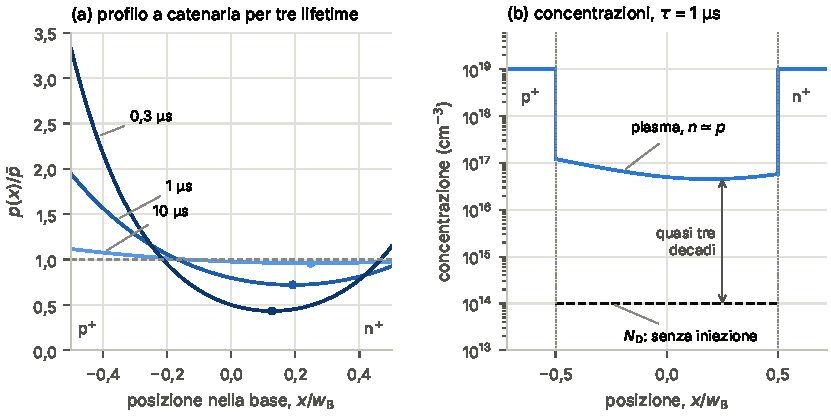
\includegraphics[width=\textwidth]{figures/fig_profile_it.pdf}
\caption{Plasma nella base di esempio a \SI{\pdExJ}{\ampere\per\centi\metre\squared}. (a) Profilo \eqref{eq:catenary} rapportato alla concentrazione media $\bar p = \tau J/(q\wB)$, per tre lifetime: $d/\La = \pdExSlowBeta$, \pdExMidBeta{} e \pdExFastBeta. Il punto è il minimo, spostato verso l'emitter \Np. (b) Concentrazioni in scala logaritmica per $\tau = \SI{\pdExMidTau}{\micro\second}$: senza iniezione la base ha solo gli elettroni del drogaggio.}
\label{fig:profile}
\end{figure}

\subsection{Caduta sulla base modulata}
\label{sec:vm}
In high injection il campo \eqref{eq:efield} è
\begin{equation}
\Ef = \frac{J}{q\,(\mun+\mup)\,p} - B\,\VT\,\frac{1}{p}\,\dpar{p}{x} .
\label{eq:fieldhl}
\end{equation}
Il primo termine è la caduta ohmica sul plasma, la cui conducibilità $\sigma = q\,(\mun+\mup)\,p$ va confrontata con quella della base senza iniezione, $\sigma_0 = q\,\mun\ND$:
\begin{equation}
\frac{\sigma}{\sigma_0} = \frac{\mun+\mup}{\mun}\,\frac{p}{\ND} \approx \pdSigmaRatio\,\frac{p}{\ND} ,
\end{equation}
cioè circa \num{\pdExMidSigRatio} alla concentrazione media dell'esempio con $\tau = \SI{\pdExMidTau}{\micro\second}$. Il secondo termine è il campo di Dember: dove la concentrazione varia, gli elettroni diffonderebbero più in fretta delle lacune, e un campo li trattiene.

La tensione sulla base è l'integrale del campo, $\VM = \int_{-d}^{d}\Ef\,\diff x$. Con il profilo \eqref{eq:catenary} l'integrale si calcola in forma chiusa (Appendice~\ref{app:vm}):
\begin{equation}
\frac{\VM}{\VT} = 2\,(1-B^2)\,\frac{\sinh\beta}{\sqrt{1-B^2\tanh^2\beta}}\,\arctan\!\Bigl(\sqrt{1-B^2\tanh^2\beta}\;\sinh\beta\Bigr)
+ B\,\ln\frac{1+B\tanh^2\beta}{1-B\tanh^2\beta} , \quad \beta = \frac{d}{\La} .
\label{eq:vm}
\end{equation}
Il primo addendo è la parte ohmica, il secondo la parte di Dember, $B\,\VT\ln[p(-d)/p(d)]$. La \eqref{eq:vm} dipende solo da $d/\La$ e dal rapporto delle mobilità: \emph{non dipende dalla corrente}. La corrente si procura da sé la conducibilità che le serve: raddoppiando $J$ raddoppia il plasma, e la resistenza si dimezza. La base modulata non si comporta come un resistore, ma come una piccola caduta costante in serie alle giunzioni. La \eqref{eq:vm} ha due limiti (Fig.~\ref{fig:vm}a e Tabella~\ref{tab:vm}).

\emph{Base sottile} ($d \ll \La$). Il profilo è quasi piatto e
\begin{equation}
\VM \simeq 2\,\VT\left(\frac{d}{\La}\right)^{2} = \frac{\wB^2\,(\mun+\mup)}{4\,\mun\mup\,\tau} ,
\label{eq:vmthin}
\end{equation}
entro il \SI{\pdVmThinErrOnePct}{\percent} fino a $d = \La$. La caduta cresce con il quadrato della larghezza della base e in proporzione inversa al lifetime. La stima che si ottiene con un profilo piatto $p = \bar p$ e la sola caduta ohmica [M]~\cite{mohan},
\begin{equation}
\VM \approx \frac{J\,\wB}{q\,(\mun+\mup)\,\bar p} = \frac{\wB^2}{(\mun+\mup)\,\tau} ,
\label{eq:vmflat}
\end{equation}
è la parte ohmica della \eqref{eq:vmthin}, cioè la frazione $1-B^2$ del totale. Con mobilità uguali le due coincidono; nel silicio la \eqref{eq:vmflat} è più bassa del \SI{\pdVmFlatLowPct}{\percent}, la parte di Dember che anche un profilo quasi piatto possiede.

\emph{Base larga} ($d \gg \La$). Il plasma si svuota al centro, dove la conducibilità è minima, e
\begin{equation}
\VM \simeq \frac{\pi}{2}\,\sqrt{1-B^2}\;\VT\,e^{d/\La} \approx \pdVmAsymCoef\;\VT\,e^{d/\La} .
\label{eq:vmwide}
\end{equation}
La caduta cresce esponenzialmente con $d/\La$. L'asintoto è raggiunto lentamente, dall'alto: a $d/\La = 3$ supera ancora il valore esatto del \SI{\pdVmAsymErrThreePct}{\percent}. Nei testi si trova spesso la forma $(3\pi/8)\,\VT\,e^{d/\La}$, scritta per $b = 3$ [M]~\cite{baliga}: manca del fattore $1/\sqrt{1-B^2}$ dell'asintoto esatto, e proprio per questo tra $d/\La = 2$ e $3$ è vicina al valore esatto (entro il \SI{\pdVmHandErrThreePct}{\percent}).

\begin{table}[htb]
\centering\small
\caption{Caduta sulla base modulata \eqref{eq:vm} con le mobilità del silicio a \SI{300}{\kelvin}, e scostamento dei due limiti e della forma dei testi.}
\label{tab:vm}
\begin{tabular}{@{}lccccc@{}}
\toprule
$d/\La$ & 0,5 & 1 & 2 & 3 & 4 \\
\midrule
$\VM/\VT$ & \pdVmHalfVt & \pdVmOneVt & \pdVmTwoVt & \pdVmThreeVt & \pdVmFourVt \\
$\VM$ a \SI{300}{\kelvin} [mV] & \pdVmHalfMv & \pdVmOneMv & \pdVmTwoMv & \pdVmThreeMv & \pdVmFourMv \\
Scostamento del limite di base sottile \eqref{eq:vmthin} & $\pdVmThinSgnHalf\,\%$ & $\pdVmThinSgnOne\,\%$ & $\pdVmThinSgnTwo\,\%$ & $\pdVmThinSgnThree\,\%$ & $\pdVmThinSgnFour\,\%$ \\
Scostamento dell'asintoto di base larga \eqref{eq:vmwide} & & & $\pdVmAsymSgnTwo\,\%$ & $\pdVmAsymSgnThree\,\%$ & $\pdVmAsymSgnFour\,\%$ \\
Scostamento della forma $(3\pi/8)\,\VT\,e^{d/\La}$ dei testi & & & $\pdVmHandSgnTwo\,\%$ & $\pdVmHandSgnThree\,\%$ & $\pdVmHandSgnFour\,\%$ \\
\bottomrule
\end{tabular}
\end{table}

\begin{figure}[htb]
\centering
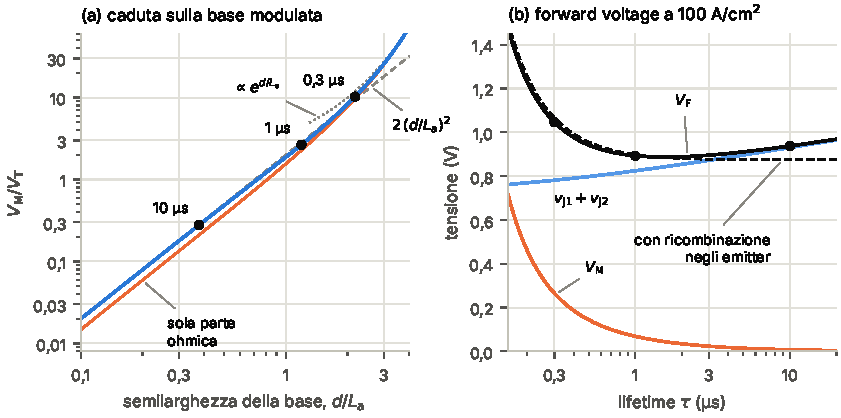
\includegraphics[width=\textwidth]{figures/fig_vm_it.pdf}
\caption{(a) Caduta sulla base modulata in unità di $\VT$ in funzione di $d/\La$: espressione esatta \eqref{eq:vm}, sua sola parte ohmica, limite di base sottile \eqref{eq:vmthin} (tratteggiato) e asintoto di base larga \eqref{eq:vmwide} (punteggiato). I punti sono i tre lifetime dell'esempio. (b) Base di esempio a \SI{\pdExJ}{\ampere\per\centi\metre\squared} in funzione del lifetime, con emitter ideali: somma delle due tensioni di giunzione, caduta $\VM$ e forward voltage $\VF$. La forward voltage ha un minimo piatto attorno a $d = \La$. Tratteggiata, $\VF$ con la ricombinazione negli emitter della Sez.~\ref{sec:emitter}.}
\label{fig:vm}
\end{figure}

La \eqref{eq:vm} vale finché valgono le sue ipotesi. Tra $10^{16}$ e $10^{17}\,\cmc$ lo scattering tra portatori comincia a ridurre le mobilità, e la caduta riprende a crescere con la corrente; la ricombinazione negli emitter (Sez.~\ref{sec:emitter}) fa crescere il plasma meno della corrente, con lo stesso effetto; a correnti molto basse, quando il plasma scende verso il drogaggio, la modulazione si perde. A questi termini si aggiungono le resistenze degli emitter, del substrato e dei contatti. È l'insieme di questi effetti a dare alla caratteristica reale una pendenza resistiva alle alte correnti.

\subsection{Tensioni di giunzione e forward characteristic}
\label{sec:vf}
La tensione ai terminali è la differenza tra il quasi-Fermi level degli elettroni al catodo e quello delle lacune all'anodo. Negli emitter, fortemente drogati, il quasi-Fermi level dei maggioritari è piatto (Sez.~\ref{sec:transport}), e attraversa piatto anche la space charge region (Sez.~\ref{sec:bias}): $\EFp$ è costante dal contatto di anodo fino al bordo $x = -d$ della base, ed $\EFn$ dal contatto di catodo fino a $x = +d$, anche con emitter non ideali. Quindi $q\,\VF = \EFn(d) - \EFp(-d)$. Nella base $n = p$, e per la \eqref{eq:qfl} la distanza tra i due livelli è $2\kB T\ln(p/\nint)$ in ogni punto; inoltre $\EFp = E_\mathrm{i} - \kB T\ln(p/\nint)$, e la differenza di $E_\mathrm{i}$ tra i due bordi è $q\VM$ per la \eqref{eq:potential}. Sommando,
\begin{equation}
\VF = \VT\,\ln\frac{p(-d)\,p(d)}{\nint^2} + \VM .
\label{eq:vfqfl}
\end{equation}
Il primo termine si divide tra le due giunzioni. Alla giunzione \Pp\Nm{} la barriera si abbassa di $\vjo$, e le lacune al bordo della base crescono del fattore di Boltzmann rispetto al loro valore di equilibrio $\nint^2/\ND$; alla giunzione \Nm\Np{} la barriera si abbassa di $\vjt$ e gli elettroni al bordo, uguali alle lacune, crescono rispetto a $\ND$:
\begin{equation}
\vjo = \VT\,\ln\frac{p(-d)\,\ND}{\nint^2} , \qquad \vjt = \VT\,\ln\frac{p(d)}{\ND} , \qquad
p(-d)\,p(d) = \nint^2\,e^{(\vjo+\vjt)/\VT} .
\label{eq:vj12}
\end{equation}
La forward voltage è quindi la somma di tre contributi,
\begin{equation}
\VF = \vjo + \VM + \vjt .
\label{eq:vfsum}
\end{equation}
La terza delle \eqref{eq:vj12} è la legge della giunzione \eqref{eq:junctionlaw} per la struttura PIN: il prodotto è preso tra i due bordi della base, e la tensione è la somma $\vj = \vjo + \vjt$ delle due tensioni di giunzione. Il drogaggio della base è scomparso: in high injection non ha più alcun ruolo nella caratteristica. Le $\vjo$ e $\vjt$ sono gli abbassamenti delle due barriere, e non le separazioni dei quasi-Fermi level ai bordi della base, che in high injection sono più grandi (Sez.~\ref{sec:bias}): in $x = -d$ la separazione è $q\,\vjo + \kB T\ln[p(-d)/\ND]$. Nell'esempio con $\tau = \SI{\pdExMidTau}{\micro\second}$ le due tensioni sono \SI{\pdExMidVjOne}{\volt} e \SI{\pdExMidVjTwo}{\volt}: la giunzione \Nm\Np{} contribuisce per un quinto, non è trascurabile. Al bordo \Pp{} i due quasi-Fermi level distano \SI{\pdExMidQflOne}{\electronvolt}, contro $q\,\vjo = \SI{\pdExMidVjOne}{\electronvolt}$.

\emph{Caratteristica.} Con le concentrazioni di bordo \eqref{eq:edges}, la terza delle \eqref{eq:vj12} lega la corrente alla somma delle tensioni di giunzione:
\begin{equation}
J = J_\mathrm{HL}\;e^{\vj/(2\VT)} , \qquad J_\mathrm{HL} = \frac{2\,q\,\Da\,\nint}{\La}\,\frac{1}{\sqrt{\coth^2\beta - B^2\tanh^2\beta}} .
\label{eq:jhl}
\end{equation}
La concentrazione di bordo cresce come $e^{\vj/(2\VT)}$, e con emitter ideali la corrente con essa: in high injection l'emission coefficient è $\Nem = 2$ (con emitter reali è più basso, Sez.~\ref{sec:emitter}). A ogni decade di corrente la tensione di giunzione cresce di $2\VT\ln 10$, circa \SI{120}{\milli\volt} a \SI{300}{\kelvin}, il doppio che in low injection. Poiché $\VM$ non dipende dalla corrente, la forward voltage è $\VF = 2\VT\ln(J/J_\mathrm{HL}) + \VM$: la caduta sulla base sposta la caratteristica di una costante. Un modello circuitale con una sola giunzione, come quello della Parte~II, la assorbe nella saturation current.

\emph{Minimo della forward voltage.} A corrente e larghezza di base fissate, dalle \eqref{eq:jhl} e \eqref{eq:vm} la forward voltage dipende dal lifetime solo attraverso $\beta$:
\begin{equation}
\frac{\VF}{\VT} = 2\,\ln\frac{J\,d}{2\,q\,\Da\,\nint} - 2\ln\beta + \ln\bigl(\coth^2\beta - B^2\tanh^2\beta\bigr) + \frac{\VM(\beta)}{\VT} .
\label{eq:vfbeta}
\end{equation}
Per una base sottile i tre termini che dipendono da $\beta$ valgono $-4\ln\beta + \tfrac{8}{3}\beta^2$, con il minimo in $\beta = \sqrt{3}/2 \approx \num{0.87}$; l'espressione esatta ha il minimo in $d/\La = \pdVfMinBeta$, qualunque siano la corrente e la larghezza. Il minimo è piatto: $\VF$ resta entro \SI{10}{\milli\volt} dal minimo per $d/\La$ da \pdVfFlatLo{} a \pdVfFlatHi{} (Fig.~\ref{fig:vm}b). Sotto il minimo, cioè per $d/\La$ più piccolo e un lifetime più lungo (a destra nella Fig.~\ref{fig:vm}b, che ha il lifetime in ascissa), $\VM$ è trascurabile e la tensione è quella delle giunzioni, che cresce con il logaritmo della concentrazione di bordo: allungare il lifetime aumenta il plasma e alza leggermente $\VF$. Sopra il minimo (a sinistra nella figura) domina $\VM$, che cresce esponenzialmente. Un fast diode sta su questo ramo: paga in forward voltage ciò che guadagna in carica. Un lifetime più lungo di quello che dà $d \approx \La$, invece, non serve alla conduzione e aggiunge solo carica da rimuovere.

\begin{table}[htb]
\centering\small
\caption{Conduzione della base di esempio ($\wB = \SI{\pdExW}{\micro\metre}$, $\ND = \pdExNd\,\cmc$) a \SI{\pdExJ}{\ampere\per\centi\metre\squared} e \SI{300}{\kelvin}, per tre lifetime. Senza iniezione la stessa base farebbe cadere \SI{\pdExDropUni}{\volt}. Le ultime tre righe sono con la ricombinazione negli emitter, $h_\mathrm{p} = h_\mathrm{n} = \pdHem\,\si{\centi\metre^4\per\second}$. La colonna con $\tau = \SI{\pdExSlowTau}{\micro\second}$ ed emitter ideali è un caso limite: alla sua concentrazione media il lifetime Auger, circa \SI{\pdExSlowTauAuger}{\micro\second}, è più breve di $\tau$, e lo scattering tra portatori ha già ridotto le mobilità. Con la ricombinazione negli emitter il plasma scende a $\pdExSlowEmPbar\,\cmc$: il lifetime Auger torna molto più lungo di $\tau$, mentre la riduzione delle mobilità per lo scattering tra portatori resta fuori dai numeri della tabella, come nelle altre due colonne (ipotesi 5, Sez.~\ref{sec:ambipolar}).}
\label{tab:conduction}
\begin{tabular}{@{}llccc@{}}
\toprule
Lifetime $\tau$ & & \SI{\pdExSlowTau}{\micro\second} & \SI{\pdExMidTau}{\micro\second} & \SI{\pdExFastTau}{\micro\second} \\
\midrule
Diffusion length $\La$; $d/\La$ & & \SI{\pdExSlowLa}{\micro\metre}; \pdExSlowBeta & \SI{\pdExMidLa}{\micro\metre}; \pdExMidBeta & \SI{\pdExFastLa}{\micro\metre}; \pdExFastBeta \\
Concentrazione media $\bar p$ [\si{\centi\metre^{-3}}] & \eqref{eq:qf} & $\pdExSlowPbar$ & $\pdExMidPbar$ & $\pdExFastPbar$ \\
Bordo \Pp, $p(-d)$ [\si{\centi\metre^{-3}}] & \eqref{eq:edges} & $\pdExSlowPl$ & $\pdExMidPl$ & $\pdExFastPl$ \\
Bordo \Np, $p(d)$ [\si{\centi\metre^{-3}}] & \eqref{eq:edges} & $\pdExSlowPr$ & $\pdExMidPr$ & $\pdExFastPr$ \\
Minimo [\si{\centi\metre^{-3}}] & & $\pdExSlowPmin$ & $\pdExMidPmin$ & $\pdExFastPmin$ \\
Stored charge $\tau J$ [\si{\micro\coulomb\per\centi\metre\squared}] & \eqref{eq:qf} & \pdExSlowQs & \pdExMidQs & \pdExFastQs \\
Conducibilità media rispetto a $\sigma_0$ & & \pdExSlowSigRatio & \pdExMidSigRatio & \pdExFastSigRatio \\
\addlinespace
Caduta sulla base $\VM$ [mV] & \eqref{eq:vm} & \pdExSlowVm & \pdExMidVm & \pdExFastVm \\
\quad di cui parte di Dember [mV] & & \pdExSlowVmDem & \pdExMidVmDem & \pdExFastVmDem \\
\quad stima a profilo piatto [mV] & \eqref{eq:vmflat} & \pdExSlowVmFlat & \pdExMidVmFlat & \pdExFastVmFlat \\
Tensioni di giunzione $\vjo$; $\vjt$ [V] & \eqref{eq:vj12} & \pdExSlowVjOne; \pdExSlowVjTwo & \pdExMidVjOne; \pdExMidVjTwo & \pdExFastVjOne; \pdExFastVjTwo \\
Forward voltage $\VF$ [V] & \eqref{eq:vfsum} & \pdExSlowVf & \pdExMidVf & \pdExFastVf \\
\addlinespace
Corrente che si ricombina negli emitter & \eqref{eq:emitterbal} & \SI{\pdExSlowEmPct}{\percent} & \SI{\pdExMidEmPct}{\percent} & \SI{\pdExFastEmPct}{\percent} \\
Lifetime efficace $Q/i$ [\si{\micro\second}] & \eqref{eq:taueff} & \pdExSlowEmTauEff & \pdExMidEmTauEff & \pdExFastEmTauEff \\
Forward voltage $\VF$ [V] & & \pdExSlowEmVf & \pdExMidEmVf & \pdExFastEmVf \\
\bottomrule
\end{tabular}
\end{table}

\subsection{Ricombinazione negli emitter e lifetime efficace}
\label{sec:emitter}
Un emitter reale non è ideale: la base vi inietta a sua volta portatori minoritari, elettroni nell'emitter \Pp{} e lacune nell'emitter \Np, che vi si ricombinano. Per la legge della giunzione \eqref{eq:junctionlaw} il prodotto $np$ è lo stesso ai due lati della space charge region; al bordo della base vale $p^2$, quindi la concentrazione dei minoritari iniettati nell'emitter è $p^2/\NA$, e la loro corrente di diffusione è proporzionale a $p^2$. Le condizioni al contorno \eqref{eq:bc} diventano \cite{schlangenotto1969}, [M]~\cite{lutz}
\begin{equation}
\Jn(-d) = q\,h_\mathrm{p}\,p^2(-d) , \qquad \Jp(d) = q\,h_\mathrm{n}\,p^2(d) ,
\label{eq:bcem}
\end{equation}
dove $h_\mathrm{p}$ e $h_\mathrm{n}$ sono i parametri di ricombinazione dei due emitter. In un emitter uniforme $h = D_\mathrm{E}/(L_\mathrm{E}\,N_\mathrm{E})$, con la diffusion constant e la diffusion length dei minoritari nell'emitter e il suo drogaggio; in un emitter reale il band-gap narrowing e la ricombinazione Auger lo aumentano, e i valori tipici sono dell'ordine di \SIrange[range-exponents=combine-bracket]{1e-14}{3e-14}{\centi\metre^4\per\second} [M]~\cite{lutz}.

Integrando la \eqref{eq:diffusion} stazionaria sulla base, con le \eqref{eq:jnjp} ai due bordi, il bilancio della corrente è
\begin{equation}
J = \frac{q\,\wB\,\bar p}{\tau} + q\,h_\mathrm{p}\,p^2(-d) + q\,h_\mathrm{n}\,p^2(d) :
\label{eq:emitterbal}
\end{equation}
la corrente alimenta la ricombinazione nella base e quella nei due emitter. La carica non è più $\tau\,\IF$. Si definisce il \emph{lifetime efficace}
\begin{equation}
\tau_\mathrm{eff} = \frac{Q}{i} = \tau\left(1 - \frac{\Jn(-d) + \Jp(d)}{J}\right) ,
\label{eq:taueff}
\end{equation}
che è più breve di $\tau$ e \emph{dipende dalla corrente}: la ricombinazione nella base cresce come $p$, quella negli emitter come $p^2$. Per la base di esempio con $\tau = \SI{\pdExMidTau}{\micro\second}$ e $h_\mathrm{p} = h_\mathrm{n} = \pdHem\,\si{\centi\metre^4\per\second}$, il profilo che soddisfa le \eqref{eq:bcem} dà negli emitter il \SI{\pdEmJLoPct}{\percent} della corrente a \SI{\pdEmJLo}{\ampere\per\centi\metre\squared}, il \SI{\pdEmJMidPct}{\percent} a \SI{\pdEmJMid}{\ampere\per\centi\metre\squared} e il \SI{\pdEmJHiPct}{\percent} a \SI{\pdEmJHi}{\ampere\per\centi\metre\squared}; il lifetime efficace scende da \SI{\pdEmJLoTauEff}{\micro\second} a \SI{\pdEmJMidTauEff}{\micro\second} e \SI{\pdEmJHiTauEff}{\micro\second}. Con un lifetime di base di \SI{\pdExSlowTau}{\micro\second} gli emitter prendono l'\SI{\pdExSlowEmPct}{\percent} della corrente e il lifetime efficace è \SI{\pdExSlowEmTauEff}{\micro\second} (Tabella~\ref{tab:conduction}): in un diodo con un lifetime lungo sono gli emitter, non la base, a fissare la carica. Le conseguenze sono cinque.
\begin{itemize}
\item La stored charge cresce meno della corrente; quando gli emitter dominano, cresce come $\sqrt{J}$.
\item La caduta sulla base non è più indipendente dalla corrente: il plasma cresce meno di $J$, e $\VM$ sale. Insieme allo scattering tra portatori è l'origine della parte resistiva della caratteristica ad alta corrente. La forward voltage ne risulta più alta dove prevale $\VM$ e più bassa con un lifetime lungo, dove le tensioni di giunzione scendono più di quanto salga $\VM$ (Tabella~\ref{tab:conduction}).
\item Anche la caratteristica \eqref{eq:jhl} cambia. La corrente che si ricombina nella base cresce come $e^{\vj/(2\VT)}$, quella che si ricombina negli emitter, $J_\mathrm{E} = \Jn(-d) + \Jp(d)$, come $e^{\vj/\VT}$: la somma delle tensioni di giunzione cresce di circa $2\VT/(1 + J_\mathrm{E}/J)$ per unità di $\ln J$, cioè con un emission coefficient tra 2 e 1. Nell'esempio a \SI{\pdExJ}{\ampere\per\centi\metre\squared} il profilo esatto dà \num{\pdExMidEmSlopeVj}\,$\VT$ con $\tau = \SI{\pdExMidTau}{\micro\second}$ e \num{\pdExSlowEmSlopeVj}\,$\VT$ con \SI{\pdExSlowTau}{\micro\second}. Ai terminali la pendenza è più alta, \num{\pdExMidEmSlopeVf}\,$\VT$ e \num{\pdExSlowEmSlopeVf}\,$\VT$, perché intanto sale $\VM$.
\item Il lifetime che un circuito vede dipende dallo stato del plasma. Una rampa di corrente rapida, che lascia più carica nella base, incontra un lifetime efficace più breve di una rampa lenta. Un modello a lifetime costante non può seguirlo: è il limite principale del modello della Parte~II (Sez.~\ref{sec:slope}).
\item L'efficienza degli emitter è una leva di progetto: un emitter debole tiene basso il plasma dal proprio lato senza toccare il lifetime della base (Sez.~\ref{sec:emittereff}).
\end{itemize}

\subsection{Temperatura}
\label{sec:temperature}
La forward characteristic ha due parti con coefficienti di temperatura opposti.

\emph{Tensioni di giunzione.} A corrente costante le concentrazioni di bordo sono fissate dalla corrente, e nelle \eqref{eq:vj12} la temperatura entra attraverso $\VT$ e $\nint$. Con la \eqref{eq:ni}, trascurando la dipendenza dalla temperatura del lifetime e delle diffusion constant,
\begin{equation}
\frac{\diff\vj}{\diff T} \approx \frac{\vj - E_\mathrm{g0}/q - 3\,\VT}{T} :
\label{eq:tc}
\end{equation}
\SI{-\pdTcLo}{\milli\volt\per\kelvin} per $\vj = \SI{\pdTcVjLo}{\volt}$ e \SI{-\pdTcHi}{\milli\volt\per\kelvin} per $\vj = \SI{\pdTcVjHi}{\volt}$, la somma delle due tensioni di giunzione dell'esempio. Il coefficiente è negativo, perché $\nint$ cresce con la temperatura, e si riduce in valore assoluto al crescere della tensione: in high injection di $2\,(\kB/q)\ln 10 \approx \SI{0.4}{\milli\volt\per\kelvin}$ per ogni decade di corrente. La stessa relazione vale in low injection, con la metà di questa variazione.

\emph{Base e parti resistive.} La caduta sulla base \eqref{eq:vmthin} è inversamente proporzionale alle mobilità, che scendono con la temperatura (Sez.~\ref{sec:ambipolar}: circa come $T^{-2,4}$ quella degli elettroni e $T^{-2,2}$ quella delle lacune, che qui pesa di più), e al lifetime, che sale: il primo effetto la aumenta, il secondo la riduce, e il risultato dipende dalla tecnologia del lifetime control. Le resistenze degli emitter e dei contatti crescono con la temperatura.

A bassa corrente prevale la giunzione e il coefficiente di temperatura di $\VF$ è negativo; ad alta corrente prevalgono la base e le parti resistive e diventa positivo. Le caratteristiche a due temperature si incrociano in un punto (\emph{crossover}). Un coefficiente positivo alla corrente di lavoro stabilizza la ripartizione della corrente tra dispositivi in parallelo; un diodo con un lifetime lungo ed emitter efficienti, cioè con $d/\La$ piccolo e $\VM$ piccola, ha il crossover a correnti alte e va verificato sul datasheet prima di metterlo in parallelo [M]~\cite{lutz}.
%=====================================================================
\part{Dinamica della carica e reverse recovery}

\section{Il reverse recovery: fenomeno e grandezze del datasheet}
\label{sec:datasheet}
La stored charge $\QF = \tau\,\IF$ che rende conduttiva la base (Sez.~\ref{sec:catenary}) va rimossa prima che il diodo possa sostenere una reverse voltage. Finché accanto alla giunzione \Pp\Nm{} resta plasma, la giunzione resta in forward bias e il diodo conduce anche in senso inverso: è il \emph{reverse recovery}. Questa sezione descrive il fenomeno e le grandezze con cui il datasheet lo misura; le sezioni successive lo descrivono con una carica (Sez.~\ref{sec:chargecontrol}) e con due (Sez.~\ref{sec:model}).

\subsection{La sequenza dello spegnimento}
\label{sec:sequence}
Lo spegnimento di un diodo avviene sempre in un circuito con un'induttanza in serie: quella di commutazione di un convertitore, o quella dispersa di un trasformatore. La Figura~\ref{fig:commcell} mostra i due circuiti a cui questo documento fa riferimento. Nella \emph{commutation cell} (a) un interruttore ideale applica la reverse voltage $\VR$ attraverso l'induttanza $\Ls$, e la corrente del diodo scende con il di/dt $a = \VR/\Ls$: è il circuito di prova dei datasheet e quello di un line-commutated converter. Nello \emph{switching leg} (b) il di/dt è imposto dall'interruttore che si accende, attraverso il suo pilotaggio, e la caduta $\Ls a$ sull'induttanza parassita è solo una parte della tensione $\Vdc$.

\begin{figure}[htb]
\centering
\begin{circuitikz}[scale=0.9, transform shape]
\ctikzset{bipoles/length=1.0cm}
% (a) commutation cell
\node[anchor=west] at (-0.9,4.2) {(a)};
\draw (0,0) to[american voltage source, invert, l=$\VR$] (0,3.2) to[closing switch, l={$t=0$}] (1.7,3.2) to[L, l=$\Ls$] (3.4,3.2) -- (6.4,3.2);
\draw (3.4,0) to[D*, l=D, *-*] (3.4,3.2);
\draw (4.9,3.2) to[R, l=$\Rsn$, *-] (4.9,1.6) to[C, l=$\Csn$, -*] (4.9,0);
\draw (6.4,3.2) to[american current source, l=$\IF$] (6.4,0);
\draw (0,0) -- (6.4,0);
\draw[-{Latex[length=2mm]}] (3.05,0.35) -- (3.05,0.95) node[midway, left]{$i$};
% (b) switching leg
\begin{scope}[xshift=9.6cm]
\node[anchor=west] at (-0.9,4.2) {(b)};
\draw (0,0) to[american voltage source, invert, l=$\Vdc$] (0,3.2) to[L, l=$\Ls$] (2.4,3.2) -- (4.6,3.2);
\draw (2.4,1.6) to[D*, l_=D, *-*] (2.4,3.2);
\draw (4.6,3.2) to[american current source, l=$I_\mathrm{L}$] (4.6,1.6) -- (2.4,1.6);
\draw (2.4,1.6) to[closing switch, l=S] (2.4,0);
\draw (0,0) -- (2.4,0);
\draw[-{Latex[length=2mm]}] (2.05,2.05) -- (2.05,2.65) node[midway, left]{$i$};
\end{scope}
\end{circuitikz}
\caption{(a) Commutation cell: il diodo conduce la corrente $\IF$ del carico; a $t=0$ l'interruttore applica la tensione $\VR$ in inverso attraverso l'induttanza $\Ls$, e la corrente del diodo scende con il di/dt $a = \VR/\Ls$. Uno snubber RC può essere posto in parallelo al diodo. (b) Switching leg: il freewheeling diode D conduce la corrente $I_\mathrm{L}$ del carico; l'interruttore S, accendendosi, la assume con un di/dt fissato dal suo pilotaggio, e $\Ls$ è l'induttanza parassita della maglia.}
\label{fig:commcell}
\end{figure}

La Figura~\ref{fig:recovery} mostra l'andamento qualitativo della corrente e della tensione. Vi si distinguono quattro fasi.
\begin{enumerate}
\item \emph{Conduzione.} Il diodo conduce $\IF$ con la forward voltage $\VF$; la base contiene il plasma della catenaria \eqref{eq:catenary} e la stored charge $\tau\,\IF$.
\item \emph{Rampa.} Il circuito porta la corrente a zero con la velocità $a$. La carica della base non segue: si riduce solo per ricombinazione, con la costante di tempo $\tau$, e allo zero della corrente ne resta una parte tanto maggiore quanto più la rampa è breve rispetto a $\tau$ (Sez.~\ref{sec:ccsolutions}).
\item \emph{Reverse current con giunzione ancora in conduzione.} La corrente si inverte e continua a crescere in modulo con lo stesso di/dt. Finché ai bordi della base c'è plasma, le due giunzioni restano in forward bias: la tensione del diodo è ancora una piccola forward voltage, benché la corrente sia invertita, e il diodo si comporta come un cortocircuito. La reverse current estrae il plasma da entrambi i lati, le lacune verso l'emitter \Pp{} e gli elettroni verso l'emitter \Np: per le condizioni al contorno \eqref{eq:bc} il gradiente al bordo \Pp\Nm{} è $b \approx 3$ volte quello al bordo \Nm\Np, quindi il lato dell'anodo si svuota circa tre volte più in fretta.
\item \emph{Interdizione e tail.} Quando la concentrazione al bordo \Pp\Nm{} scende a zero, la giunzione non può più fornire la corrente che il circuito chiede: si forma una space charge region, il diodo assume tensione e la reverse current raggiunge il picco $\Irr$. Nella cella della Fig.~\ref{fig:commcell}a il picco è l'istante in cui la reverse voltage del diodo, $v_\mathrm{R} = -v$, vale $\VR$, perché $\Ls\,\diff i/\diff t = v_\mathrm{R} - \VR$ si annulla lì. Il plasma rimasto, che in una base non larga rispetto a $\La$ si trova verso il catodo (Sez.~\ref{sec:onenumber}), continua a fornire corrente mentre viene rimosso dalla ricombinazione, dalla diffusione verso i bordi e dall'avanzare della space charge region: è la \emph{tail}. Nella tail la corrente decresce in modulo, e l'induttanza aggiunge la sua tensione a quella del circuito: la reverse voltage supera $\VR$ e raggiunge un picco, che senza capacità in parallelo al diodo è la $\Vrm$ della \eqref{eq:vrm} e con una capacità cambia (Sez.~\ref{sec:energy}).
\end{enumerate}

\begin{figure}[htb]
\centering
\begin{tikzpicture}[x=1.3cm, y=1.5cm, >={Latex[length=2mm]}, font=\small]
% fasi
\foreach \x in {1,2.25,3.156} \draw[gray!70, densely dotted] (\x,-3.4) -- (\x,1.5);
\node at (0.5,1.38) {1}; \node at (1.62,1.38) {2}; \node at (2.7,1.38) {3}; \node at (4.6,1.38) {4};
% --- corrente
\fill[gray!25] (2.25,0) -- (3.0,-0.6) .. controls (3.1,-0.68) and (3.2,-0.68) .. (3.35,-0.6)
   -- plot[domain=3.35:8.0, samples=60] (\x,{-0.6*exp(-(\x-3.35)/0.9)}) -- (8.0,0) -- cycle;
\draw[->] (0,0) -- (8.5,0) node[right] {$t$};
\draw[->] (0,-0.9) -- (0,1.3) node[above] {$i$};
\draw[thick] (0,1) -- (1,1) -- (3.0,-0.6) .. controls (3.1,-0.68) and (3.2,-0.68) .. (3.35,-0.6)
   -- plot[domain=3.35:8.0, samples=60] (\x,{-0.6*exp(-(\x-3.35)/0.9)});
\node[left] at (0,1) {$\IF$};
\node[anchor=west, fill=white, inner sep=1.5pt] (slope) at (0.1,0.45) {$\diff i/\diff t = -a$};
\draw[->] (slope.east) -- (1.66,0.47);
\draw[<->] (3.156,0) -- (3.156,-0.66);
\node[right] at (3.17,-0.3) {$\Irr$};
\node (qrr) at (5.0,-0.6) {$\Qrr$};
\draw[thin] (qrr.north west) -- (3.9,-0.17);
\draw[<->] (2.25,0.16) -- (3.156,0.16) node[midway, above] {$\ta$};
\draw[<->] (3.156,0.16) -- (5.0,0.16) node[midway, above] {$\tb$};
\draw[gray!70, densely dotted] (5.0,-0.2) -- (5.0,0.75);
\draw[<->] (2.25,0.62) -- (5.0,0.62) node[midway, above] {$\trr$};
% --- tensione inversa
\begin{scope}[yshift=-4.6cm]
\draw[->] (0,0) -- (8.5,0) node[right] {$t$};
\draw[->] (0,-0.25) -- (0,1.55) node[above] {$v_\mathrm{R} = -v$};
\draw[gray, dashed] (0,0.75) -- (8.2,0.75);
\node[left] at (0,0.75) {$\VR$};
\draw[thick] (0,-0.06) -- (2.8,-0.06) plot[smooth, tension=0.55] coordinates {(2.8,-0.06) (2.95,0.04) (3.06,0.38) (3.156,0.75) (3.27,1.08) (3.42,1.24) (3.6,1.2) (3.9,1.05) (4.4,0.9) (5.2,0.8) (6.2,0.76) (8.0,0.75)};
\node[below] at (1.4,-0.06) {$-\VF$};
\draw[<->] (3.42,0) -- (3.42,1.24);
\node[right] at (3.6,1.3) {$\Vrm$};
\end{scope}
\end{tikzpicture}
\caption{Andamento qualitativo dello spegnimento di un diodo PIN su una rampa di corrente: corrente e reverse voltage $v_\mathrm{R} = -v$. I numeri indicano le fasi descritte nel testo; il confine tra le fasi 3 e 4 è tracciato al picco della corrente, poco dopo l'inizio dell'interdizione. L'area grigia è la recovered charge. La fine del recovery, e quindi $\tb$ e $\trr$, richiede una convenzione (Sez.~\ref{sec:rrdata}).}
\label{fig:recovery}
\end{figure}

Tre osservazioni preparano le sezioni che seguono. La prima: la reverse current non è un difetto della giunzione ma la rimozione di una carica, e la sua entità dipende da quanta carica la rampa ha lasciato nella base, non dalla carica statica. La seconda: l'istante dell'interdizione è deciso dalla concentrazione a \emph{un bordo}, non dalla carica totale; è per questo che una sola carica non basta a descrivere il recovery, e che la forma del profilo conta quanto il suo integrale. La terza: nella tail è il diodo a imporre la corrente e il circuito a subirla, e tutto ciò che è pericoloso nel recovery (sovratensione, oscillazioni, dynamic avalanche) accade lì.
\subsection{Le grandezze del recovery}
\label{sec:rrdata}
Nella prova di recovery il diodo conduce dapprima la forward current $\IF$. Il circuito forza poi la corrente a scendere con velocità costante $a = -\diff i/\diff t$, attraverso lo zero e nel verso inverso (Fig.~\ref{fig:waveform}a, che mostra la forma d'onda del modello a due cariche della Sez.~\ref{sec:model}). La reverse current sale fino al picco $\Irr$, che raggiunge al tempo $\ta$ dopo lo zero della corrente; il diodo assume quindi la reverse voltage $\VR$ e la corrente torna a zero nel tempo $\tb$. Il datasheet fornisce alcune delle grandezze seguenti, con le condizioni di prova $\IF$, $a$, $\VR$ e la temperatura di giunzione.
\begin{itemize}
\item \emph{Peak reverse recovery current} $\Irr$ ($I_\mathrm{rrm}$ nella IEC~60747-2 \cite{iec60747}, 3.3.10; $I_\mathrm{RM}$ o $I_\mathrm{RR}$ in molti datasheet).
\item \emph{Recovered charge} $\Qrr$ ($Q_\mathrm{r}$ in \cite{iec60747}, 3.5.5; anche $Q_\mathrm{S}$): l'integrale della reverse current a partire dallo zero della corrente. La norma termina l'integrale all'istante in cui la corrente è scesa al \SI{\lmPEndPct}{\percent} del picco, e osserva che la carica comprende componenti dovute sia al carrier storage sia alla junction capacitance (3.5.5, Nota~2). Alcuni datasheet la chiamano stored charge; in questo documento la stored charge è la carica presente nella base, di cui la recovered charge è una parte.
\item \emph{Reverse recovery time} $\trr = \ta + \tb$ (\cite{iec60747}, 3.5.2), dallo zero della corrente alla fine del recovery. La corrente tende a zero in modo asintotico, quindi la fine richiede una convenzione. La norma traccia una retta per due punti A e B della corrente in discesa e prende l'istante in cui la retta raggiunge lo zero; A è spesso specificato al \SI{90}{\percent} e B al \SI{25}{\percent} del picco (3.5.2, Nota~5). La stessa costruzione si trova in \cite{an6481}, Sez.~2.1. Altri documenti prendono l'istante in cui la corrente è scesa a una frazione del picco: il \SI{10}{\percent} nella documentazione dei simulatori \cite{mathworks,plecs}, una frazione $k$, di solito \num{0.25}, in \cite{an5028}. La norma chiama le due parti di $\trr$ rise time e fall time (3.5.3, 3.5.4).
\item \emph{Softness}: il rapporto $\tb/\ta$ (\cite{an6481}, Sez.~2.1; \cite{an5028}), oppure un rapporto tra i due di/dt della reverse current, prima e dopo il picco. I termini soft e snappy sono definiti nella Sez.~\ref{sec:softsnappy}.
\end{itemize}
I diodi raddrizzatori per frequenza di rete sono di solito forniti con $\Qrr$ e $\Irr$ massime alla massima temperatura di giunzione e a un di/dt di pochi \Aus, e con le curve delle due grandezze in funzione del di/dt. I fast diode sono forniti con $\Irr$, $\Qrr$ e $\trr$ tipiche a due temperature e a centinaia o migliaia di \Aus, con curve in funzione della forward current e del di/dt.

\begin{figure}[htb]
\centering
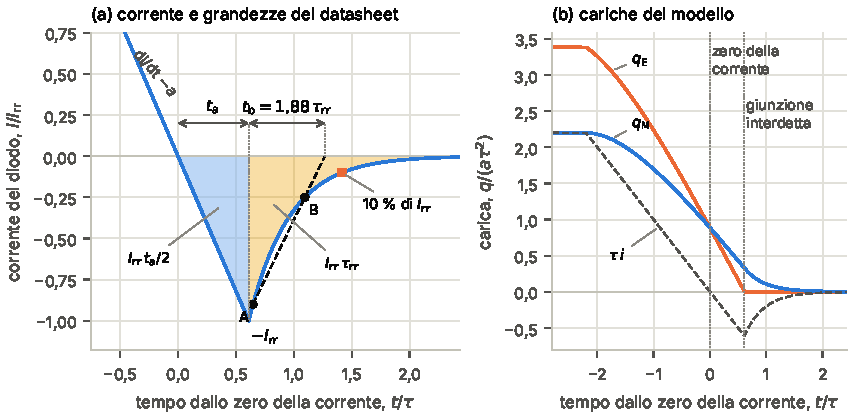
\includegraphics[width=\textwidth]{../lauritzen_ma_datasheet_conversion/figures/fig_waveform_it.pdf}
\caption{Spegnimento del modello a due cariche (Sez.~\ref{sec:model}) su una rampa di corrente ($\rho = \taurr/\tau = \lmFigRho$, $\IF/(a\tau) = \lmFigLam$). (a) Corrente e grandezze del datasheet: il triangolo di carica $\Irr\ta/2$, la tail di carica $\Irr\taurr$, la retta per i punti A (\SI{90}{\percent}) e B (\SI{25}{\percent}) che definisce $\tb$, e il punto al \SI{10}{\percent}. (b) Le due cariche del modello e, tratteggiata, $\tau i$: la middle charge $\qM$ segue la corrente con un ritardo, l'edge charge $\qE$ raggiunge lo zero dopo la corrente, e in quell'istante la giunzione entra in interdizione.}
\label{fig:waveform}
\end{figure}

\subsection{Forward characteristic nel datasheet}
Per un diodo raddrizzatore il datasheet fornisce la forward voltage a una corrente e un'approssimazione lineare della caratteristica alla massima temperatura,
\begin{equation}
v \approx \VTo + \rT\, i ,
\label{eq:line}
\end{equation}
con la threshold voltage $\VTo$, da non confondere con la thermal voltage $\VT$, e la slope resistance $\rT$. La retta interseca la caratteristica reale a due correnti, che il datasheet dichiara o che sono implicite nel campo di validità della retta. Per un fast diode il datasheet fornisce la forward voltage alla corrente nominale e una curva a due temperature.

\subsection{Blocking state nel datasheet}
Il datasheet fornisce la reverse current $\Irrm$ alla repetitive peak reverse voltage $\Vrrm$ e alla massima temperatura, come valore massimo; è una corrente statica, da non confondere con il picco di recovery, che la norma indica con $I_\mathrm{rrm}$. Una junction capacitance è data per i diodi piccoli e veloci, a bassa reverse voltage; per i grandi diodi raddrizzatori di solito non è data.
\subsection{Soft e snappy}
\label{sec:softsnappy}
Il modo in cui la corrente torna a zero dopo il picco decide la sovratensione. Nella tail $\diff i/\diff t > 0$, e la reverse voltage del diodo è $v_\mathrm{R} = \VR + \Ls\,\diff i/\diff t$: la sovratensione è proporzionale alla rapidità con cui la tail si estingue.

Un diodo è \emph{soft} se nella base resta plasma finché la space charge region ha raggiunto l'estensione che compete alla tensione applicata: la corrente decade allora con la costante di tempo del plasma residuo, e la sovratensione è contenuta. È \emph{snappy} se il plasma si esaurisce mentre scorre ancora una reverse current rilevante: la corrente si interrompe in un tempo molto breve (\emph{snap-off}), la sovratensione è elevata, fino a portare la reverse voltage oltre la $\Vrrm$ del diodo, e l'induttanza oscilla con la junction capacitance del diodo, con le interferenze elettromagnetiche (EMI) che ne seguono.

Alle due misure della softness della Sez.~\ref{sec:rrdata} questo documento preferisce il rapporto $s$ tra la carica della tail e quella del triangolo, \eqref{eq:soft}; nel modello a due cariche, su una rampa lunga, vale $2\TM/\tau$, dove il transit time $\TM$ del modello è dell'ordine del tempo di diffusione sulla semilarghezza della base, $d^2/(3\Da)$ (Sezz.~\ref{sec:lumped} e~\ref{sec:onenumber}). Va letto per ciò che è: $s$ misura la forma di una tail di diffusione, e nessuna di queste misure prevede lo snap-off. Il modello a due cariche non lo contiene, perché la sua tail è sempre un esponenziale; e a geometria fissata $2\TM/\tau$ cresce quando si riduce il lifetime, senza che un diodo reale diventi per questo più soft.

Le condizioni che favoriscono lo snap-off si leggono sulla fisica della Parte~I [M]~\cite{lutz}.
\begin{itemize}
\item \emph{Base sottile.} In una base punch-through o con field stop la space charge region raggiunge la fine della base alla tensione $q\ND\wB^2/(2\varepsilon)$, \SI{\pdExVrt}{\volt} per la base di esempio (\SI{\pdExW}{\micro\metre}, $\pdExNd\,\cmc$). Se la tensione applicata la supera, la space charge region spazza l'intera base e il plasma residuo non ha dove restare.
\item \emph{Tensione alta}, per la stessa ragione; \emph{corrente bassa} e \emph{temperatura bassa}, perché la stored charge è minore; \emph{di/dt alto} e \emph{induttanza alta}, perché la tensione sale prima e di più.
\end{itemize}
Ne segue una regola di verifica: le perdite, $\Qrr$ e $\Irr$ vanno prese alla massima temperatura di giunzione e alla corrente nominale; la sovratensione e la softness vanno verificate anche a bassa temperatura e a bassa corrente, dell'ordine di un decimo della nominale, con la tensione più alta.

Per il recovery conta quindi la distribuzione del plasma oltre alla sua quantità. Il plasma accanto alla giunzione \Pp\Nm{} va rimosso prima che la giunzione possa entrare in interdizione, e fissa $\Irr$; il plasma sul lato del catodo alimenta la tail, e fissa la softness. Le tecnologie della Sez.~\ref{sec:technology} agiscono su questa distribuzione.

\subsection{Dynamic avalanche}
\label{sec:dynaval}
Durante il recovery la space charge region si forma mentre la reverse current la attraversa. In essa la corrente è portata da lacune che viaggiano verso l'emitter \Pp{} a una velocità prossima a quella di saturazione, $v_\mathrm{sat} \approx \SI{e7}{\centi\metre\per\second}$ [M]~\cite{sze}, con la concentrazione
\begin{equation}
p = \frac{J}{q\,v_\mathrm{sat}} .
\label{eq:pdyn}
\end{equation}
La loro carica si somma a quella dei donori, e la \eqref{eq:poisson} dà
\begin{equation}
\dpar{\Ef}{x} = \frac{q}{\varepsilon}\,(\ND + p) .
\label{eq:dynfield}
\end{equation}
La base si comporta come se il suo drogaggio fosse $\ND + p$: il campo ha un gradiente più ripido e raggiunge il valore critico a una tensione più bassa. A \SI{\pdDynJLo}{\ampere\per\centi\metre\squared} la \eqref{eq:pdyn} dà $p = \pdDynPLo\,\cmc$, il \SI{\pdDynPctLo}{\percent} del drogaggio della base di esempio: con la \eqref{eq:ecrit} e un campo triangolare il valore critico è raggiunto a circa \SI{\pdDynVbrLo}{\volt}, contro i \SI{\pdBlkVC}{\volt} dello stesso drogaggio senza corrente (Tabella~\ref{tab:blocking}) e i \SI{\pdExVbr}{\volt} statici della base di esempio, che è punch-through. A \SI{\pdDynJHi}{\ampere\per\centi\metre\squared} è raggiunto a circa \SI{\pdDynVbrHi}{\volt}.

È la \emph{dynamic avalanche}: una generazione per impatto a tensioni ben inferiori alla breakdown voltage statica, presente solo mentre scorre la reverse current. Una dynamic avalanche moderata si autolimita, perché gli elettroni generati attraversano la space charge region e compensano in parte la carica delle lacune; una forte può concentrare la corrente in filamenti e distruggere il diodo [M]~\cite{lutz}. È ciò che limita il prodotto tra reverse current e tensione durante il recovery, cioè la \emph{safe operating area} (SOA) del diodo in reverse recovery, che alcuni datasheet riportano, e con essa il di/dt ammesso alle tensioni più alte.

\subsection{Forward recovery}
\label{sec:forwardrec}
Al turn-on del diodo avviene il fenomeno opposto. Se la corrente sale più in fretta di quanto il plasma impieghi a formarsi, la base è ancora quella senza iniezione, con la resistenza $R_\mathrm{B} = \wB/(q\,\mun\,\ND)$ della \eqref{eq:runi}: \SI{\pdExRuni}{\ohm\centi\metre\squared} per la base di esempio, cioè \SI{\pdExDropUni}{\volt} a \SI{\pdExJ}{\ampere\per\centi\metre\squared}, e \SI{\pdTgtDrop}{\volt} per la base non-punch-through da \SI{\pdTgtV}{\kilo\volt} della Sez.~\ref{sec:why}. Sono i limiti superiori, per una corrente applicata a gradino. La tensione del diodo ha quindi un picco $V_\mathrm{FRM}$ (\emph{forward recovery}), che può valere decine o centinaia di volt, e scende poi a $\VF$ mentre il plasma riempie la base. Il tempo caratteristico è quello della diffusione del plasma nella base, dell'ordine del transit time $d^2/(3\Da)$ della Sez.~\ref{sec:lumped} (\SI{\pdExTmPar}{\nano\second} per la base di esempio), non del lifetime. Il picco cresce con il di/dt, con la larghezza della base, cioè con la classe di tensione, e con la temperatura, perché la mobilità scende [M]~\cite{lutz}; a esso si somma la caduta induttiva del package.

Il forward recovery conta dove un diodo deve assumere corrente in fretta: nei diodi di clamp e di snubber, la cui tensione di picco si somma a quella che dovrebbero limitare, e nel freewheeling diode al turn-off dell'interruttore. Il modello a due cariche non lo riproduce (Sez.~\ref{sec:otherlimits}).
%=====================================================================
\section{Il modello a controllo di carica}
\label{sec:chargecontrol}
Il modello più semplice della dinamica del diodo descrive l'intera base con un solo numero, la stored charge $Q = qA\int p\,\diff x$. Discende dall'equazione di diffusione ambipolare senza approssimazioni ulteriori, e ne conserva ciò che nel dominio del tempo conta di più: il ritardo con cui la carica segue la corrente. È anche il modello di carica del diodo di SPICE, con il parametro \texttt{TT} al posto di $\tau$ (Sez.~\ref{sec:others}).

\subsection{Derivazione}
\label{sec:ccderiv}
Si integri la \eqref{eq:diffusion} sulla base, da $-d$ a $+d$, e si moltiplichi per $qA$:
\begin{equation}
\frac{\diff Q}{\diff t} = q\,A\,\Da\left[\dpar{p}{x}\right]_{-d}^{+d} - \frac{Q}{\tau} .
\label{eq:integrated}
\end{equation}
Il primo termine è il flusso di plasma che entra dai due bordi. Con le condizioni al contorno \eqref{eq:bc} degli emitter ideali vale $q A \Da\,J\,[1/(2q\Dn) + 1/(2q\Dp)] = A\,J = i$, per la \eqref{eq:da}. Ne segue l'\emph{equazione del controllo di carica}
\begin{equation}
\frac{\diff Q}{\diff t} = i - \frac{Q}{\tau} .
\label{eq:cc}
\end{equation}
La corrente alimenta la carica, la ricombinazione la consuma. In regime stazionario ogni portatore iniettato si ricombina nella base, e $i = Q/\tau$: la corrente di un diodo PIN non è un transito di portatori da un terminale all'altro, ma l'alimentazione di una ricombinazione.

\emph{In una riga.} Lo stesso risultato si ottiene integrando sulla base l'equazione di continuità delle lacune \eqref{eq:contp}, con $U = p/\tau$: $\diff Q/\diff t = A\,[\Jp(-d) - \Jp(+d)] - Q/\tau$. Con emitter ideali $\Jp(-d) = J$ e $\Jp(+d) = 0$, ed è di nuovo la \eqref{eq:cc}. Questa via mostra che l'equazione non richiede l'high injection, la quasi-neutralità, un drogaggio uniforme, mobilità costanti o una forma del profilo. Richiede tre cose:
\begin{itemize}
\item \emph{emitter ideali}. Con la ricombinazione negli emitter della Sez.~\ref{sec:emitter} il bilancio diventa
\begin{equation}
\frac{\diff Q}{\diff t} = i - \frac{Q}{\tau} - q\,A\,\bigl[h_\mathrm{p}\,p^2(-d) + h_\mathrm{n}\,p^2(d)\bigr] ,
\label{eq:ccem}
\end{equation}
e la carica statica è $\tau_\mathrm{eff}\,\IF$ con il lifetime efficace \eqref{eq:taueff}, che scende al crescere della corrente: $\QF = \tau\,\IF$ è un limite superiore;
\item \emph{ricombinazione lineare} con un solo $\tau$. Il lifetime di Shockley--Read--Hall passa da $\tau_\mathrm{p0}$ in low injection a $\tau_\mathrm{p0} + \tau_\mathrm{n0}$ in high injection (Sez.~\ref{sec:lifetime}): la \eqref{eq:cc} vale attraverso i due regimi solo con un $\tau$ che dipende dal livello di iniezione;
\item che $i$ sia la corrente di conduzione. Quando la giunzione entra in interdizione alla corrente ai terminali si aggiunge quella della junction capacitance, $\Cj\,\diff v/\diff t$.
\end{itemize}

\subsection{Soluzioni notevoli}
\label{sec:ccsolutions}
\emph{Regime stazionario.} Con $\diff Q/\diff t = 0$ la \eqref{eq:cc} dà la \eqref{eq:qf}, $\QF = \tau\,\IF$. Con la caduta sulla base sottile \eqref{eq:vmthin} il prodotto
\begin{equation}
\VM\,\QF = \frac{\wB^2\,(\mun+\mup)}{4\,\mun\,\mup}\;\IF
\label{eq:tradeoff}
\end{equation}
non dipende dal lifetime: è il compromesso fondamentale del diodo bipolare. A parità di base, ogni riduzione della stored charge si paga con un aumento proporzionale della caduta sulla base; per la base di esempio $\VM\,\tau = \SI{\pdExVmTau}{\milli\volt\micro\second}$. La sola via per ridurre entrambe è una base più sottile.

\emph{Circuito aperto.} Se la corrente è interrotta, $i = 0$ e
\begin{equation}
Q(t) = \QF\,e^{-t/\tau} :
\label{eq:opencircuit}
\end{equation}
la carica scompare per sola ricombinazione. Senza corrente i gradienti ai bordi sono nulli, il profilo si appiattisce e la concentrazione ai bordi segue la carica; con la legge della giunzione in high injection, $p \propto e^{\vj/(2\VT)}$ (Sez.~\ref{sec:vf}), la tensione ai terminali scende linearmente,
\begin{equation}
\frac{\diff\vj}{\diff t} = -\frac{2\,\VT}{\tau} ,
\label{eq:ocvd}
\end{equation}
cioè di \SI{\pdOcvdSlope}{\milli\volt\per\micro\second} per $\tau = \SI{1}{\micro\second}$ a \SI{300}{\kelvin}. Quando la base torna in low injection la pendenza diventa $-\VT/\tau_\mathrm{p0}$: scompare il fattore 2 e il lifetime è quello di low injection, quindi la pendenza si dimezza solo se i due lifetime coincidono. È il metodo di misura del lifetime per \emph{open-circuit voltage decay} \cite{schroder}: a differenza delle misure di recovery, non richiede di conoscere la forma del profilo.

\emph{Reverse current costante.} Se a $t = 0$ la corrente passa da $\IF$ a $-\IR$ e il circuito la mantiene, la \eqref{eq:cc} dà $Q(t) = -\tau\,\IR + \tau\,(\IF + \IR)\,e^{-t/\tau}$. La carica si annulla allo \emph{storage time}
\begin{equation}
\ts = \tau\,\ln\Bigl(1 + \frac{\IF}{\IR}\Bigr) ,
\label{eq:storage}
\end{equation}
che vale \num{\pdTsOne}\,$\tau$ per $\IR = \IF$ e \num{\pdTsFour}\,$\tau$ per $\IR = \IF/4$. È la relazione classica per stimare $\tau$ da una prova di commutazione resistiva. Il $\tau$ che se ne ricava è una stima per difetto: la giunzione entra in interdizione quando si annulla la concentrazione al bordo, prima che si annulli la carica, e lo storage time reale è più breve di quello della \eqref{eq:storage}. Il modello a due cariche ne dà una stima migliore, \eqref{eq:ts}.

\emph{Rampa di corrente.} È il caso dello spegnimento in un convertitore. Con $i(t) = \IF - a\,t$ e il valore iniziale $\tau\,\IF$,
\begin{equation}
Q(t) = \tau\,(\IF - a\,t) + a\,\tau^2\,\bigl(1 - e^{-t/\tau}\bigr) .
\label{eq:ccramp}
\end{equation}
Il primo termine è la carica che la base avrebbe se seguisse la corrente senza ritardo; il secondo è il ritardo, carica ancora presente perché la ricombinazione richiede tempo. Allo zero della corrente, $t_0 = \IF/a$, il primo termine si annulla:
\begin{equation}
Q(t_0) = a\,\tau^2\,\bigl(1 - e^{-\IF/(a\tau)}\bigr) .
\label{eq:qzero}
\end{equation}
La carica presente allo zero della corrente non è la carica statica. Il rapporto $Q(t_0)/\QF = (1 - e^{-\lambda})/\lambda$ dipende solo da $\lambda = \IF/(a\tau)$, il tempo che la rampa impiega a raggiungere lo zero della corrente, in unità di lifetime: è il \SI{\pdRampFracFast}{\percent} per $\lambda = \num{\pdRampLamFast}$, il \SI{\pdRampFracMid}{\percent} per $\lambda = 1$ e il \SI{\pdRampFracSlow}{\percent} per $\lambda = 5$. Su una rampa lunga $Q(t_0) = a\,\tau^2$, qualunque sia la forward current: la carica iniziale si è ricombinata lungo il percorso, e ciò che resta è quanto hanno alimentato gli ultimi lifetime della rampa.

Con una sola carica la giunzione entra in interdizione quando $Q = 0$. Dalla \eqref{eq:ccramp}, all'istante $\Tone = (\IF + \Irr)/a$,
\begin{equation}
\Irr = a\,\tau\,\bigl(1 - e^{-\Tone/\tau}\bigr) , \qquad \Qrr = \frac{\Irr^2}{2a} :
\label{eq:ccpeak}
\end{equation}
la reverse current è un triangolo che si interrompe al picco. Su una rampa lunga $\Irr = a\,\tau$ e $\Qrr = a\,\tau^2/2$, metà della \eqref{eq:qzero}: l'altra metà si ricombina durante $\ta$. Su una rampa brevissima, $a\tau \gg \IF$, $\Irr \to \sqrt{2\,a\,\tau\,\IF}$ e $\Qrr \to \tau\,\IF$. Per le tre rampe di prima la recovered charge è il \SI{\pdRampQrrFast}{\percent}, il \SI{\pdRampQrrMid}{\percent} e il \SI{\pdRampQrrSlow}{\percent} di $\tau\,\IF$. La stima $\Qrr \approx \tau\,\IF$ vale quindi solo per commutazioni molto rapide; a basso di/dt sovrastima la carica di molto, e un lifetime letto come $\Qrr/\IF$ è sottostimato nella stessa misura.

\subsection{Il diodo come sistema del primo ordine}
\label{sec:ccsystem}
La \eqref{eq:cc} è lineare. Tra la corrente e la carica c'è la funzione di trasferimento
\begin{equation}
\frac{Q(j\omega)}{i(j\omega)} = \frac{\tau}{1 + j\omega\,\tau} ,
\label{eq:cctf}
\end{equation}
un filtro passa-basso con la costante di tempo $\tau$. Per variazioni di corrente lente rispetto al lifetime la carica segue in modo quasi statico, $Q \simeq \tau\,i$; per variazioni rapide la base integra la corrente e la carica non fa in tempo a cambiare. Un diodo raddrizzatore a frequenza di rete, con $\tau$ di decine di microsecondi e un periodo di \SI{20}{\milli\second}, è nel primo caso fino agli ultimi lifetime prima dello zero; un fast diode commutato in \SI{100}{\nano\second} con $\tau$ di alcune centinaia di nanosecondi è nel secondo, e allo zero della corrente contiene ancora gran parte della carica statica.

\subsection{Limiti del modello a una carica}
\label{sec:cclimits}
\begin{enumerate}
\item \emph{Nessuna tail.} Il recovery finisce quando $Q = 0$, con una corrente che cade a zero in un tempo nullo: il modello non ha softness, e in un circuito con un'induttanza dà una sovratensione infinita. In un diodo reale la giunzione entra in interdizione prima, quando si svuota il bordo, e la carica rimasta nella base alimenta la tail.
\item \emph{Nessuna forma.} La carica totale non dice dove si trova il plasma. Il modello non distingue un profilo piatto da uno svuotato al bordo, e non può descrivere né l'istante dell'interdizione né il forward recovery.
\item \emph{Lifetime costante.} Il lifetime efficace dipende dalla corrente, per la ricombinazione negli emitter (Sez.~\ref{sec:emitter}) e per il passaggio da low a high injection, e dalla temperatura. La ricombinazione Auger nella base conta solo oltre circa $3\times10^{17}\,\cmc$ (Sez.~\ref{sec:lifetime}).
\end{enumerate}
Il primo e il secondo limite si superano aggiungendo una seconda variabile che descriva il bordo della base: è il modello della prossima sezione. Il terzo resta anche lì (Sez.~\ref{sec:limits}).

\emph{Nota sull'IGBT.} La stessa equazione descrive la carica della base di un IGBT, con una differenza nelle condizioni al contorno: sul lato opposto all'emitter \Pp{} non c'è un emitter \Np, ma la giunzione del p-well, che raccoglie le lacune, e il canale MOS, che fornisce alla base la corrente di elettroni $I_\mathrm{n,MOS}$. Integrando sulla base la continuità degli elettroni, con un emitter \Pp{} ideale, si ottiene $\diff Q/\diff t = I_\mathrm{n,MOS} - Q/\tau$: a regime la carica è $\tau$ volte la corrente del canale, non la corrente di collettore. Quando il canale si spegne, $I_\mathrm{n,MOS} = 0$ e la carica residua decade come $e^{-t/\tau}$; la corrente di tail, proporzionale alla carica residua, decade con la stessa costante di tempo. Un lifetime efficace più breve di $\tau$, come quello che si osserva in pratica, viene da ciò che queste ipotesi escludono: l'emitter non ideale, la ricombinazione nel buffer, la base neutra che si restringe mentre la tensione sale [M]~\cite{baliga}.
%=====================================================================
\addtocontents{toc}{\protect\enlargethispage{\baselineskip}}\section{Il modello a due cariche di Lauritzen--Ma}
\label{sec:model}
Il modello di Lauritzen e Ma \cite{lauritzen1991} aggiunge all'equazione del controllo di carica una seconda variabile, che descrive il bordo della base. È il modello con dinamica di carica di diversi simulatori di circuito (Sez.~\ref{sec:others}), per esempio \cite{mathworks}, e il componente \texttt{diode\_rr} della libreria pwr-control ne è un'implementazione. Questa sezione lo ricava dalla fisica della Parte~I, ne scrive le equazioni e ne discute i due regimi; le Sezioni~\ref{sec:ramp} e~\ref{sec:direct} lo risolvono su una rampa di corrente.

\subsection{Dalla base a due lumped charge}
\label{sec:lumped}
La derivazione segue l'idea delle lumped charge di Linvill \cite{linvill1958}, che \cite{lauritzen1991} applica al diodo; la scelta del profilo qui sotto è un modo di farlo, non una citazione dell'articolo.

Si descriva il profilo del plasma con una parabola,
\begin{equation}
p(x,t) = c_0 + c_1\,\frac{x}{d} + c_2\,\frac{x^2}{d^2} , \qquad -d \leq x \leq d .
\label{eq:parabola}
\end{equation}
La concentrazione media è $\bar p = c_0 + c_2/3$, e la media delle concentrazioni ai due bordi è $p_\mathrm{E} = c_0 + c_2$. Le condizioni al contorno \eqref{eq:bc} legano i coefficienti alla corrente: la differenza dei due gradienti dà $4\,\Da\,c_2/d = J/q$, la loro somma dà $c_1 = -B\,J\,d/(2\,q\,\Da)$. Si definiscano due cariche: la \emph{middle charge}, che è l'intera stored charge, e l'\emph{edge charge}, la carica che la base conterrebbe se la concentrazione di bordo la riempisse:
\begin{equation}
\qM = Q = 2\,q\,A\,d\,\bar p , \qquad \qE = 2\,q\,A\,d\,p_\mathrm{E} .
\label{eq:lumpeddef}
\end{equation}
Allora $\qE - \qM = \tfrac43\,qAd\,c_2$, e la corrente è
\begin{equation}
i = \frac{4\,q\,A\,\Da\,c_2}{d} = \frac{\qE - \qM}{\TM} , \qquad \TM = \frac{d^2}{3\,\Da} = \frac{\wB^2}{12\,\Da} .
\label{eq:tmgeom}
\end{equation}
La corrente è la diffusione dai bordi verso il centro, e il \emph{transit time} $\TM$ è il tempo di diffusione sulla semilarghezza della base: \SI{\pdExTmPar}{\nano\second} per la base di esempio. La \eqref{eq:tmgeom} vale per qualunque rapporto delle mobilità, purché $p_\mathrm{E}$ sia la media dei due bordi. Insieme all'equazione del controllo di carica \eqref{eq:cc}, che è esatta, dà le due equazioni dinamiche del modello.

\emph{Legge della giunzione.} Per la \eqref{eq:vj12} il prodotto delle concentrazioni ai due bordi segue la somma $\vj$ delle due tensioni di giunzione, $p(-d)\,p(d) = \nint^2\,e^{\vj/\VT}$. Per un profilo simmetrico $p_\mathrm{E} = \nint\,e^{\vj/(2\VT)}$: l'edge charge segue la junction voltage con l'emission coefficient $\Nem = 2$. Una reverse voltage porta a zero la concentrazione di bordo e non può fare di più: è la giunzione interdetta, $\qE = 0$.

\emph{Asimmetria.} Con mobilità diverse i due bordi non sono uguali. Il termine lineare della \eqref{eq:parabola} dà
\begin{equation}
p(\mp d) = p_\mathrm{E} \pm 3B\,(p_\mathrm{E} - \bar p) , \qquad \text{cioè, in termini di cariche,} \qquad \qE \pm 3B\,\TM\,i :
\label{eq:edgesasym}
\end{equation}
in conduzione diretta il bordo \Pp{} è più alto della media, in reverse current è più basso. Nella legge della giunzione entra il prodotto dei due bordi, $p_\mathrm{E}^2 - 9B^2\,(p_\mathrm{E}-\bar p)^2$, in cui l'asimmetria compare solo al secondo ordine: in conduzione la legge scritta con $p_\mathrm{E}$ resta una buona descrizione. L'asimmetria conta invece per l'istante dell'interdizione, che è deciso dal solo bordo \Pp{} (Sez.~\ref{sec:onenumber}).
\subsection{Equazioni}
Raccogliendo i risultati della Sez.~\ref{sec:lumped}, il modello descrive i portatori immagazzinati nella base con due cariche (Fig.~\ref{fig:model}). La \emph{middle charge} $\qM$ è la stored charge nella base. L'\emph{edge charge} $\qE$ rappresenta la concentrazione dei portatori ai bordi della base, accanto alla giunzione, ed è legata alla junction voltage. I portatori diffondono dal bordo verso il centro, e questa diffusione è la corrente del diodo:
\begin{align}
\idif &= \frac{\qE - \qM}{\TM} , \label{eq:idif}\\
\frac{\diff \qM}{\diff t} &= \idif - \frac{\qM}{\tau} , \label{eq:qm}\\
\qE &= (\tau+\TM)\,\IS\,\bigl(e^{\vj/(\Nem\VT)} - 1\bigr) . \label{eq:qe}
\end{align}
L'equazione \eqref{eq:qm} è il bilancio della middle charge: la diffusion current la alimenta e la ricombinazione la rimuove con il lifetime $\tau$. L'equazione \eqref{eq:idif} dice che la corrente è sostenuta dalla differenza tra le due cariche e che $\TM$ è il tempo che i portatori impiegano a diffondere nella base. L'equazione \eqref{eq:qe} è la legge della giunzione (junction law) della Sez.~\ref{sec:lumped}, scritta per l'edge charge. Il diodo completo aggiunge la junction capacitance, una leakage resistance e una resistenza serie:
\begin{equation}
i = \idif + \Cj(\vj)\,\frac{\diff \vj}{\diff t} + \frac{\vj}{\Rr} , \qquad v = \vj + \RS\, i .
\label{eq:terminal}
\end{equation}
Il modello ha un solo stato per la stored charge, $\qM$, perché $\qE$ è una funzione algebrica della junction voltage. Sono le equazioni di \cite{lauritzen1991}; la \eqref{eq:tmgeom} dice che cosa è $\TM$ in termini di larghezza della base.

Nella \eqref{eq:qe} il fattore davanti alla parentesi è scritto in modo che $\IS$ sia la saturation current della caratteristica statica, come in \cite{mathworks}. Alcune implementazioni, tra cui il componente di libreria \texttt{diode\_rr}, scrivono $\qE = \tau\,\IS^{*}\,(e^{\vj/(\Nem\VT)}-1)$. Le due forme sono lo stesso modello con
\begin{equation}
\IS^{*} = \IS\,\frac{\tau+\TM}{\tau} .
\label{eq:isstar}
\end{equation}
\begin{figure}[htb]
\centering
\begin{circuitikz}[scale=0.9, transform shape]
\ctikzset{bipoles/length=1.0cm}
\draw (0,0) node[left]{A} to[short, o-] (0.3,0) to[R, l=$\RS$] (2.3,0) coordinate (J);
\draw (J) -- (2.3,1.5) to[american controlled current source, l={$\idif$}] (5.3,1.5) -- (5.3,0) coordinate (K);
\draw (J) to[C, l=$\Cj(\vj)$, *-*] (K);
\draw (J) -- (2.3,-1.5) to[R, l=$\Rr$] (5.3,-1.5) -- (K);
\draw (K) to[short, -o] (6.2,0) node[right]{K};
\draw[-{Latex[length=2mm]}] (0.4,0.42) -- (0.95,0.42) node[midway, above]{$i$};
\node at (2.55,-2.0) {$+$}; \node at (3.8,-2.0) {$\vj$}; \node at (5.05,-2.0) {$-$};
\end{circuitikz}
\caption{Circuito equivalente del modello: la diffusion current $\idif = (\qE-\qM)/\TM$, con $\qM$ dalla \eqref{eq:qm} e $\qE$ dalla \eqref{eq:qe}, in parallelo alla junction capacitance e alla leakage resistance, e in serie a $\RS$.}
\label{fig:model}
\end{figure}
\subsection{Caratteristica statica}
In regime stazionario $\diff\qM/\diff t = 0$, quindi le \eqref{eq:idif} e \eqref{eq:qm} danno
\begin{equation}
\qM = \tau\, i , \qquad \qE = (\tau+\TM)\, i , \qquad i = \IS\,\bigl(e^{\vj/(\Nem\VT)}-1\bigr) .
\label{eq:static}
\end{equation}
A riposo il modello è l'ordinaria equazione del diodo con una resistenza serie, e la base contiene la carica $\tau\,i$. I parametri $\IS$, $\Nem$ e $\RS$ danno forma alla forward characteristic e non hanno alcun ruolo nel recovery, purché la forward voltage sia piccola rispetto alle tensioni del circuito.

\emph{Legame con la fisica.} La \eqref{eq:static} con $\Nem = 2$ è la caratteristica \eqref{eq:jhl} della base in high injection con emitter ideali. La junction voltage del modello è $\vjo+\vjt+\VM$: comprende la caduta sulla base, che con emitter ideali non dipende dalla corrente e sposta la caratteristica senza cambiarne la pendenza, e la saturation current corrisponde a $\IS \approx A\,J_\mathrm{HL}\,e^{-\VM/(2\VT)}$. La ricombinazione negli emitter porta la pendenza della parte di giunzione sotto $2\VT$ e fa crescere $\VM$ con la corrente (Sez.~\ref{sec:emitter}); insieme alla riduzione delle mobilità e alle resistenze degli emitter, dei contatti e del package, finisce in $\RS$ e in un emission coefficient di fit diverso da 2 (Sez.~\ref{sec:forward}).
\subsection{Due regimi e due costanti di tempo}
\label{sec:regimes}
Il diodo lavora in uno di due regimi.

\emph{Giunzione in conduzione} ($\qE > 0$). La junction voltage è una forward voltage dell'ordine di un volt, qualunque sia il segno della corrente. Il circuito impone la corrente, e le cariche la seguono: con $\idif = i$,
\begin{equation}
\frac{\diff \qM}{\diff t} = i - \frac{\qM}{\tau} , \qquad \qE = \qM + \TM\, i .
\label{eq:conducting}
\end{equation}
La prima relazione è l'equazione del controllo di carica \eqref{eq:cc}. La seconda dice che l'edge charge è la middle charge più una parte proporzionale alla corrente. In questo regime può scorrere una reverse current: basta che sia $\qM > \TM\,|i|$.

\emph{Giunzione interdetta} ($\qE = 0$). L'edge charge non può scendere sotto zero: nella \eqref{eq:qe} una reverse voltage porta la parentesi a $-1$ e $\qE$ a $-(\tau+\TM)\IS$, che è nulla sulla scala della stored charge. Con $\qE = 0$,
\begin{equation}
\idif = -\frac{\qM}{\TM} , \qquad \frac{\diff\qM}{\diff t} = -\qM\Bigl(\frac1\TM + \frac1\tau\Bigr) = -\frac{\qM}{\taurr} , \qquad \taurr = \frac{\tau\,\TM}{\tau+\TM} .
\label{eq:blocked}
\end{equation}
Il diodo è ora un generatore di corrente che decade con la costante di tempo $\taurr$, qualunque cosa faccia il circuito; il circuito impone la tensione. La carica rimasta nella base esce per diffusione verso i bordi (la reverse current) e per ricombinazione, e le due velocità si sommano. La tail time constant è sempre più breve sia di $\tau$ sia di $\TM$. Il rapporto
\begin{equation}
\rho = \frac{\taurr}{\tau} = \frac{\TM}{\tau+\TM}
\label{eq:rho}
\end{equation}
è usato nel seguito come parametro di forma del modello, con $0 < \rho < 1$.

Vista dalla corrente, l'edge charge della giunzione in conduzione è una copia filtrata della corrente. Dalle \eqref{eq:conducting}, in regime sinusoidale,
\begin{equation}
\frac{\qE(j\omega)}{i(j\omega)} = (\tau+\TM)\,\frac{1+j\omega\,\taurr}{1+j\omega\,\tau} .
\label{eq:filter}
\end{equation}
È una rete ritardatrice. Per una corrente che varia lentamente sulla scala di $\tau$ è un puro ritardo di $\tau-\taurr$: l'edge charge è $(\tau+\TM)$ volte la corrente che scorreva un tempo $\tau-\taurr$ prima. La giunzione entra in interdizione quando $\qE$ attraversa lo zero, quindi su una rampa lenta lo fa $\tau-\taurr$ dopo lo zero della corrente, quando la reverse current è cresciuta fino ad $a\,(\tau-\taurr)$. È l'intero reverse recovery del modello in una riga; la Sezione~\ref{sec:ramp} lo rende esatto.

La \eqref{eq:filter} misura anche quanto il modello approssima la base distribuita. Si definisca l'edge charge della base distribuita come nella \eqref{eq:lumpeddef}, con la media delle concentrazioni ai due bordi. Per qualunque rapporto delle mobilità, la \eqref{eq:diffusion} con le condizioni al contorno \eqref{eq:bc} dà tra la corrente e questa carica la risposta esatta
\begin{equation}
\frac{\qE(j\omega)}{i(j\omega)} = \tau\,\frac{\beta\,\coth(\beta\gamma)}{\gamma} , \qquad \gamma = \sqrt{1+j\omega\tau} , \qquad \beta = \frac{d}{\La} ,
\label{eq:distributed}
\end{equation}
e la \eqref{eq:filter} con $\TM = d^2/(3\Da)$ ne è lo sviluppo al primo ordine in $\beta^2\gamma^2$: un polo e uno zero al posto di una funzione trascendente. Per questa carica, media dei due bordi, il modello a due cariche è quindi esatto per una base sottile rispetto alla diffusion length e per frequenze ben sotto $1/\TM$; diventa un'approssimazione, da tarare sulla forma d'onda, quando $d$ si avvicina a $\La$. L'istante dell'interdizione dipende però dal solo bordo \Pp: con mobilità diverse il transit time che lo riproduce non è la \eqref{eq:tmgeom}, nemmeno per una base sottile (Sez.~\ref{sec:onenumber}).
\subsection{Quanto può fare un solo numero}
\label{sec:onenumber}
Il transit time della \eqref{eq:tmgeom} viene da un profilo parabolico. La base distribuita ha altri stati, e ciascuno richiede un valore diverso. Questa sezione li confronta con la soluzione esatta della \eqref{eq:diffusion}, nelle stesse ipotesi: emitter ideali, lifetime costante, e una space charge region di larghezza trascurabile rispetto alla base.

\emph{Regime stazionario.} Il profilo esatto è la catenaria \eqref{eq:catenary}. Per $\omega = 0$ la \eqref{eq:distributed} dà $\qE = \tau\,\beta\coth\beta\;i$, mentre $\qM = \tau\,i$; il confronto con le \eqref{eq:static} dà, per qualunque rapporto delle mobilità,
\begin{equation}
\frac{\TM}{\tau} = \beta\,\coth\beta - 1 ,
\label{eq:tmstatic}
\end{equation}
che vale $\beta^2/3$, cioè $\TM = d^2/(3\Da)$, per una base più stretta della diffusion length, e cresce meno in fretta per una base larga: \num{\pdExSlowTmStat}, \num{\pdExMidTmStat} e \num{\pdExFastTmStat} per i tre lifetime della Tabella~\ref{tab:conduction}.

\emph{Rampa lunga: l'istante dell'interdizione.} Durante il recovery conta un solo bordo, quello \Pp, e nel silicio, dove $b \approx 3$, il profilo non è simmetrico. Per la \eqref{eq:edgesasym} il bordo \Pp{} si svuota quando $\qE = 3B\,\TM\,|i|$, non quando $\qE = 0$: in quell'istante la carica rimasta nella base è
\begin{equation}
\qM = (1 + 3B)\,\frac{d^2}{3\,\Da}\,|i| ,
\label{eq:tmasym}
\end{equation}
cioè $1 + 3B \approx \num{\pdTmAsymFactor}$ volte quella che dà la \eqref{eq:tmgeom}. È il risultato della parabola, e vale per una base sottile. Per una base qualunque la risposta esatta del bordo \Pp{} alla corrente è
\begin{equation}
\frac{2\,q\,A\,d\;p(-d,j\omega)}{i(j\omega)} = \tau\,\frac{\beta\,\bigl[\coth(\beta\gamma) + B\,\tanh(\beta\gamma)\bigr]}{\gamma} ,
\label{eq:edgeresponse}
\end{equation}
di cui la \eqref{eq:distributed} è la parte simmetrica. Su una rampa lunga la concentrazione al bordo segue la corrente con un ritardo, che è la derivata logaritmica della \eqref{eq:edgeresponse} rispetto a $j\omega$, cambiata di segno e calcolata in $\omega = 0$. Il bordo si svuota quindi al tempo
\begin{equation}
\frac{\ta}{\tau} = \frac12\left[1 + \frac{\beta\,\bigl(1/\sinh^2\beta - B/\cosh^2\beta\bigr)}{\coth\beta + B\,\tanh\beta}\right]
\label{eq:tadist}
\end{equation}
dopo lo zero della corrente, e la peak reverse current è $\Irr = a\,\ta$. Nel modello a due cariche lo stesso ritardo è $\tau - \taurr = \tau^2/(\tau+\TM)$ (Sez.~\ref{sec:regimes}). Il transit time che riproduce il picco di una base distribuita è quindi
\begin{equation}
\TM = \tau\,\Bigl(\frac{\tau}{\ta} - 1\Bigr) ,
\label{eq:tmeff}
\end{equation}
ed è anche il rapporto tra la carica rimasta nella base all'interdizione e la corrente di picco, perché la \eqref{eq:cc} è esatta. Per una base sottile la \eqref{eq:tmeff} tende alla \eqref{eq:tmasym}; per una base larga $\ta \to \tau/2$ e $\TM \to \tau$, qualunque sia la larghezza.

\emph{Tail.} Dopo l'interdizione la concentrazione al bordo \Pp{} resta nulla. Le \eqref{eq:bc} valgono ancora, con la corrente fissata ora dal diodo: la giunzione interdetta non inietta elettroni e la giunzione \Nm\Np{} non lascia passare lacune, quindi i gradienti ai due bordi restano nel rapporto $b$. Il modo più lento della \eqref{eq:diffusion} con queste condizioni è
\begin{equation}
p \propto \sin\frac{\theta\,(x+d)}{2\,d}\;e^{-t/\taurr} , \qquad \cos\theta = -\frac1b , \qquad \frac{1}{\taurr} = \frac1\tau + \frac{\theta^2\,\Da}{4\,d^2} ,
\end{equation}
e il confronto con $1/\taurr = 1/\tau + 1/\TM$ dà
\begin{equation}
\TM = \frac{4\,d^2}{\theta^2\,\Da} .
\label{eq:tmtail}
\end{equation}
Con mobilità uguali $\theta = \pi$, il modo è un coseno nullo ai due bordi e $\TM = 4d^2/(\pi^2\Da)$, il \SI{\pdTmModeRatioPct}{\percent} sopra la \eqref{eq:tmgeom}; con le mobilità del silicio $\theta = \num{\pdTmTailAngle}$ e $\TM = \num{\pdTmTailCoef}\,d^2/\Da$, \num{\pdTmTailFactor} volte la \eqref{eq:tmgeom}. La tail di una base distribuita non è però un solo esponenziale: il profilo all'interdizione contiene anche i modi più rapidi, e all'inizio la corrente decade più in fretta. Ciò che entra in $\Qrr$ e nell'energia \eqref{eq:erec} è la carica della tail, cioè la softness \eqref{eq:soft}; la si ottiene senza integrare nel tempo, con una quadratura sul profilo all'interdizione (Appendice~\ref{app:scripts}). La tensione di picco dipende invece dal di/dt iniziale della tail, che in una base distribuita è più alto di quello dell'esponenziale di uguale carica: la \eqref{eq:vrm} vale per una tail esponenziale, e con questa softness sottostima il picco.

\begin{table}[htb]
\centering\small
\caption{Base distribuita con emitter ideali e lifetime costante su una rampa lunga, per $b = \num{\pdBratio}$: istante dell'interdizione, transit time efficace e softness esatti, e ciò che ne ricava la conversione della Sez.~\ref{sec:invpq} applicata al picco e alla carica esatti.}
\label{tab:distributed}
\begin{tabular}{@{}lccccccc@{}}
\toprule
$d/\La$ & \num{0.25} & \num{0.5} & 1 & \num{1.5} & 2 & 3 & $\infty$ \\
\midrule
$\ta/\tau$, \eqref{eq:tadist} & \pdDistTaQuarter & \pdDistTaHalf & \pdDistTaOne & \pdDistTaOneHalf & \pdDistTaTwo & \pdDistTaThree & $1/2$ \\
$\TM/\tau$ efficace, \eqref{eq:tmeff} & \pdDistTmQuarter & \pdDistTmHalf & \pdDistTmOne & \pdDistTmOneHalf & \pdDistTmTwo & \pdDistTmThree & 1 \\
\quad in unità di $d^2/(3\Da)$ & \pdDistTmGeomQuarter & \pdDistTmGeomHalf & \pdDistTmGeomOne & \pdDistTmGeomOneHalf & \pdDistTmGeomTwo & \pdDistTmGeomThree & 0 \\
Softness $s$ & \pdDistSQuarter & \pdDistSHalf & \pdDistSOne & \pdDistSOneHalf & \pdDistSTwo & \pdDistSThree & 1 \\
\addlinespace
Conversione: lifetime restituito, rispetto a $\tau$ & \pdDistTauFitQuarter & \pdDistTauFitHalf & \pdDistTauFitOne & \pdDistTauFitOneHalf & \pdDistTauFitTwo & \pdDistTauFitThree & $3/4$ \\
Conversione: transit time restituito, rispetto a $\tau$ & \pdDistTmFitQuarter & \pdDistTmFitHalf & \pdDistTmFitOne & \pdDistTmFitOneHalf & \pdDistTmFitTwo & \pdDistTmFitThree & $3/8$ \\
\quad larghezza che la \eqref{eq:tmgeom} gli attribuisce, rispetto a $\wB$ & \pdDistWidthQuarter & \pdDistWidthHalf & \pdDistWidthOne & \pdDistWidthOneHalf & \pdDistWidthTwo & \pdDistWidthThree & 0 \\
\bottomrule
\end{tabular}
\end{table}

La Tabella~\ref{tab:distributed} raccoglie questi risultati per una rampa lunga, e aggiunge ciò che la conversione della Sez.~\ref{sec:invpq} restituisce quando le si danno il picco e la carica esatti. Con mobilità uguali il transit time efficace è \num{\pdTmBlockSymQuarter}, \num{\pdTmBlockSymHalf} e \num{\pdTmBlockSymOne} volte $d^2/(3\Da)$ per $d/\La = \num{0.25}$, \num{0.5} e 1: fino a $d \approx \La$ lo scostamento dalla \eqref{eq:tmgeom} viene quasi tutto dall'asimmetria. Dalla tabella si leggono tre cose.
\begin{itemize}
\item \emph{Base sottile.} Fino a $d \approx \La/2$ la conversione restituisce il lifetime entro l'\SI{1}{\percent} e un transit time vicino alla \eqref{eq:tmasym}: letto con la \eqref{eq:tmgeom}, corrisponde a una base larga circa una volta e mezza quella vera. La softness è bassa, perché la tail è breve rispetto al triangolo.
\item \emph{Base larga.} Oltre $d \approx \num{1.5}\,\La$ il ritardo tende a $\tau/2$ e la softness a 1, con un massimo di \num{\pdDistSmax} attorno a $d/\La = \num{\pdDistSmaxBeta}$ (\num{\pdDistSmaxSym} attorno a $d/\La = \num{\pdDistSmaxBetaSym}$ con mobilità uguali): il recovery non dipende più dalla larghezza della base. La conversione restituisce circa tre quarti del lifetime, e un transit time vicino a $3\tau/8$ che non contiene più alcuna informazione sulla base.
\item \emph{Dove resta il plasma.} All'interdizione il plasma residuo di una base sottile ha il massimo in $x = +B\,d$, a metà strada tra il centro e il catodo: la carica è rimossa prima dal lato \Pp, come nella descrizione della Sez.~\ref{sec:sequence}. Il massimo è a $+\num{\pdTmPeakPosHalf}\,d$ per $d/\La = \num{0.5}$ e a $+\num{\pdTmPeakPosOne}\,d$ per $d/\La = 1$; oltre $d/\La \approx \num{\pdTmPeakZeroBeta}$ passa nella metà dell'anodo. In una base larga i due bordi si svuotano quasi insieme, e il plasma residuo resta più alto dal lato dell'anodo, come in conduzione.
\end{itemize}

Il transit time è quindi dell'ordine di $d^2/\Da$ per una base sottile, tra \num{0.33} e \num{\pdTmTailCoef} volte questo valore a seconda dello stato che deve descrivere, e dell'ordine di $\tau$ per una base larga. In nessun caso è una costante calcolabile dalla geometria: è un parametro efficace, da ricavare dalla forma d'onda di recovery, e per una base larga lo è anche il lifetime. Con emitter ideali e lifetime costante, inoltre, la softness su una rampa lunga non supera \num{\pdDistSmax}. Un valore ben maggiore di 1 non è compatibile con queste ipotesi: viene dalle tecnologie della Sez.~\ref{sec:technology} che tengono plasma dal lato del catodo, e i due parametri che lo riproducono sono allora behavioural (Sez.~\ref{sec:exrec}).
\subsection{Parametri}
\begin{table}[htb]
\centering\small
\caption{Parametri del modello e dati del datasheet che li fissano.}
\label{tab:params}
\begin{tabular}{@{}ll>{\raggedright\arraybackslash}p{6.4cm}c@{}}
\toprule
Parametro & Ruolo & Dati del datasheet & Sezione \\
\midrule
$\tau$, $\TM$ & reverse recovery & due tra $\Irr$, $\Qrr$, $\trr$ a di/dt e forward current dichiarati & \ref{sec:inverse} \\
$\IS$, $\Nem$, $\RS$ & forward characteristic & $\VTo$ e $\rT$, oppure punti della forward curve & \ref{sec:forward} \\
$\Rr$ & leakage nel blocking state & reverse current a una reverse voltage & \ref{sec:blocking} \\
$\Cjo$, $\Vbi$, $m_\mathrm{j}$ & junction capacitance & capacità a una reverse voltage, oppure una stima & \ref{sec:blocking} \\
\bottomrule
\end{tabular}
\end{table}
I quattro gruppi della Tabella~\ref{tab:params} sono indipendenti: ciascuno si può convertire senza gli altri. I parametri del recovery sono l'oggetto delle prossime tre sezioni.

%=====================================================================
\section{Spegnimento su una rampa di corrente}
\label{sec:ramp}
\subsection{Ipotesi}
Il diodo è in regime stazionario con la forward current $\IF$. Da $t = 0$ il circuito forza la corrente a scendere con la velocità costante $a$:
\begin{equation}
i(t) = \IF - a\,t .
\label{eq:ramp}
\end{equation}
Nella commutation cell della Fig.~\ref{fig:commcell}a il di/dt è $a = \VR/\Ls$. Il circuito impone la rampa finché la giunzione conduce, perché la junction voltage è piccola rispetto a $\VR$. La junction capacitance e il leakage sono trascurati in questa sezione; la Sezione~\ref{sec:cell} mostra il loro effetto sui due esempi.

\subsection{Cariche durante la rampa}
Finché la giunzione conduce, la middle charge obbedisce all'equazione del controllo di carica, e sulla rampa segue la \eqref{eq:ccramp}; l'edge charge segue dalla seconda delle \eqref{eq:conducting}:
\begin{align}
\qM(t) &= \tau\,(\IF - a\,t) + a\,\tau^2\,\bigl(1 - e^{-t/\tau}\bigr) , \label{eq:qmramp}\\
\qE(t) &= (\tau+\TM)\,(\IF - a\,t) + a\,\tau^2\,\bigl(1 - e^{-t/\tau}\bigr) . \label{eq:qeramp}
\end{align}
Allo zero della corrente, $t_0 = \IF/a$, le due cariche sono uguali e valgono la \eqref{eq:qzero}, $a\,\tau^2\,(1 - e^{-\IF/(a\tau)})$: non la carica statica $\tau\IF$ ma, su una rampa che dura diversi lifetime, $a\,\tau^2$, qualunque sia la forward current. La Figura~\ref{fig:waveform}b mostra le due cariche.
\subsection{Peak reverse current}
La giunzione entra in interdizione all'istante $\Tone$ in cui $\qE$ raggiunge lo zero. La corrente in quell'istante è il picco, $i(\Tone) = -\Irr$, quindi $\Tone = (\IF+\Irr)/a$. L'equazione \eqref{eq:qeramp} con $\qE(\Tone) = 0$, e con $\tau^2/(\tau+\TM) = \tau - \taurr$, dà
\begin{equation}
\Irr = a\,(\tau-\taurr)\,\bigl(1 - e^{-\Tone/\tau}\bigr) , \qquad \Tone = \frac{\IF+\Irr}{a} .
\label{eq:peak}
\end{equation}
È un'equazione implicita in $\Irr$, perché $\Tone$ la contiene. Il tempo dallo zero della corrente al picco è $\ta = \Irr/a$. Fino al picco la tensione del diodo è ancora una piccola forward voltage, benché la corrente sia già invertita.

\subsection{Tail e recovered charge}
Dopo $\Tone$ la giunzione è interdetta e valgono le \eqref{eq:blocked}, con $\qM(\Tone) = \TM\Irr$:
\begin{equation}
i(t) = -\Irr\,e^{-(t-\Tone)/\taurr} , \qquad t \geq \Tone .
\label{eq:tail}
\end{equation}
La reverse current è un triangolo di base $\ta$ seguito da un esponenziale, con uno spigolo al picco. Il suo integrale è la recovered charge
\begin{equation}
\Qrr = \frac{\Irr\,\ta}{2} + \Irr\,\taurr = \frac{\Irr^2}{2a} + \Irr\,\taurr .
\label{eq:qrr}
\end{equation}
L'equazione \eqref{eq:qrr} vale per qualunque durata della rampa: usa solo la forma d'onda.

\subsection{Forma normalizzata e soluzione in forma chiusa}
\label{sec:norm}
Con le grandezze normalizzate
\begin{equation}
y = \frac{\Irr}{a\,\tau} , \qquad \lambda = \frac{\IF}{a\,\tau} , \qquad \rho = \frac{\taurr}{\tau} ,
\label{eq:normdef}
\end{equation}
le equazioni \eqref{eq:peak} e \eqref{eq:qrr} diventano
\begin{equation}
y = (1-\rho)\,\bigl(1 - e^{-(\lambda+y)}\bigr) , \qquad \frac{\Qrr}{a\,\tau^2} = \frac{y^2}{2} + \rho\,y .
\label{eq:norm}
\end{equation}
Il recovery normalizzato dipende da due soli numeri: il parametro di forma $\rho$, e $\lambda$, che è il tempo impiegato dalla rampa per raggiungere lo zero della corrente contato in lifetime. La prima delle \eqref{eq:norm} ha la soluzione
\begin{equation}
y = (1-\rho) + W_0\!\left(-(1-\rho)\,e^{-(\lambda+1-\rho)}\right) ,
\label{eq:lambert}
\end{equation}
dove $W_0$ è il ramo principale della funzione di Lambert, l'inversa di $z \mapsto z\,e^{z}$ (Appendice~\ref{app:lambert}). Il termine di Lambert è negativo: è ciò che la durata finita della rampa toglie al valore per rampa lunga $1-\rho$. La Figura~\ref{fig:map} mostra il risultato.

\begin{figure}[htb]
\centering
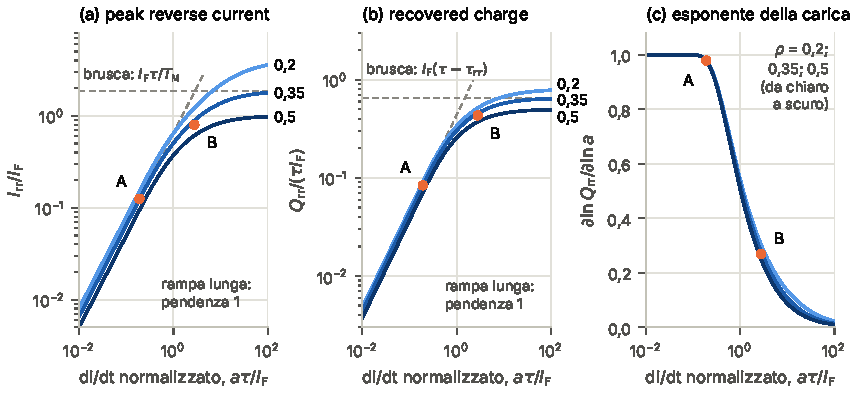
\includegraphics[width=\textwidth]{../lauritzen_ma_datasheet_conversion/figures/fig_map_it.pdf}
\caption{Recovery del modello in funzione del di/dt normalizzato $a\tau/\IF = 1/\lambda$, per tre valori di $\rho$. (a) Peak reverse current e (b) recovered charge, con i due asintoti della curva centrale: la rampa lunga \eqref{eq:long}, con pendenza uno, e la commutazione brusca \eqref{eq:abrupt}, una costante. (c) Esponente locale della carica rispetto al di/dt, \eqref{eq:exponents}. I punti A e B sono i due esempi svolti della Sez.~\ref{sec:examples} nelle loro condizioni di datasheet.}
\label{fig:map}
\end{figure}

\subsection{Rampa lunga e commutazione brusca}
\label{sec:limitsramp}
\emph{Rampa lunga} ($\lambda \to \infty$). L'esponenziale della \eqref{eq:peak} si annulla:
\begin{equation}
\Irr = a\,(\tau - \taurr) = \frac{a\,\tau^2}{\tau+\TM} , \qquad \ta = \tau - \taurr , \qquad \Qrr = \frac{a}{2}\,\bigl(\tau^2 - \taurr^2\bigr) .
\label{eq:long}
\end{equation}
Picco e carica sono proporzionali al di/dt e non dipendono dalla forward current. Il tempo al picco è una costante del diodo: è il ritardo $\tau - \taurr$ della \eqref{eq:filter}.

Il fattore $1 - e^{-\xi}$ della \eqref{eq:peak}, con $\xi = \Tone/\tau$, dice quanto deve essere lunga una rampa. La Tabella~\ref{tab:long} riporta quanto manca ai valori per rampa lunga. Ai fini di una conversione una rampa è lunga quando dura cinque lifetime dalla forward current al picco; con tre lifetime le formule per rampa lunga sbagliano del \SI{\lmFDefThree}{\percent} sul picco e fino all'\SI{\lmQDefHiThree}{\percent} sulla carica.

\begin{table}[htb]
\centering\small
\caption{Corrente di picco e carica del modello su una rampa di durata finita, rispetto ai valori per rampa lunga \eqref{eq:long}. L'intervallo della carica è per $\rho$ da 0,5 a 0,1.}
\label{tab:long}
\begin{tabular}{@{}lcccc@{}}
\toprule
Durata della rampa, $\xi = \Tone/\tau$ & 2 & 3 & 4 & 5 \\
\midrule
$\Irr$: quanto manca al valore per rampa lunga & \SI{\lmFDefTwo}{\percent} & \SI{\lmFDefThree}{\percent} & \SI{\lmFDefFour}{\percent} & \SI{\lmFDefFive}{\percent} \\
$\Qrr$: quanto manca al valore per rampa lunga & \SIrange{\lmQDefLoTwo}{\lmQDefHiTwo}{\percent} & \SIrange{\lmQDefLoThree}{\lmQDefHiThree}{\percent} & \SIrange{\lmQDefLoFour}{\lmQDefHiFour}{\percent} & \SIrange{\lmQDefLoFive}{\lmQDefHiFive}{\percent} \\
\bottomrule
\end{tabular}
\end{table}

\emph{Commutazione brusca} ($\lambda \to 0$). La rampa è così rapida che nulla si ricombina prima che la giunzione entri in interdizione. La middle charge è ancora $\tau\IF$ quando l'edge charge è portata a zero, e la \eqref{eq:blocked} dà
\begin{equation}
\Irr \to \IF\,\frac{\tau}{\TM} , \qquad \Qrr \to \IF\,(\tau - \taurr) = \IF\,\frac{\tau^2}{\tau+\TM} .
\label{eq:abrupt}
\end{equation}
Picco e carica sono proporzionali alla forward current e non dipendono più dal di/dt. Sono i valori più grandi che il modello può dare per una data forward current.

\subsection{Bilancio della carica}
Della carica presente allo zero della corrente, \eqref{eq:qzero}, solo una parte esce dai terminali. Il resto si ricombina durante il recovery. Su una rampa lunga, dalla \eqref{eq:long},
\begin{equation}
\frac{\Qrr}{\qM(t_0)} = \frac{1-\rho^2}{2} .
\label{eq:fraction}
\end{equation}
Viene recuperata meno della metà della carica presente allo zero della corrente: il \SI{\lmQfracRhoLo}{\percent} per $\rho = 0,2$, il \SI{\lmQfracRhoMid}{\percent} per $\rho = 0,35$, il \SI{\lmQfracRhoHi}{\percent} per $\rho = 0,5$. In una commutazione brusca la parte recuperata della carica statica $\tau\IF$ è $1-\rho$, per la \eqref{eq:abrupt}. La recovered charge di un datasheet non è quindi mai la stored charge del diodo, e il lifetime non si può leggere come $\Qrr/\IF$ (Sez.~\ref{sec:others}).

\subsection{Dipendenza dal di/dt e dalla forward current}
\label{sec:exponents}
Finché la giunzione conduce, le equazioni \eqref{eq:conducting} sono lineari, e la condizione di interdizione $\qE = 0$ non cambia se la corrente e le cariche sono tutte moltiplicate per lo stesso fattore. Quindi se il di/dt e la forward current sono entrambi moltiplicati per $c$, l'intera forma d'onda è moltiplicata per $c$: $\Irr$ e $\Qrr$ sono funzioni omogenee di grado uno della coppia $(a, \IF)$, come mostrano le \eqref{eq:normdef} e \eqref{eq:norm}. Per il teorema di Eulero sulle funzioni omogenee
\begin{equation}
\frac{\partial \ln \Irr}{\partial \ln a} + \frac{\partial \ln \Irr}{\partial \ln \IF} = 1 , \qquad
\frac{\partial \ln \Qrr}{\partial \ln a} + \frac{\partial \ln \Qrr}{\partial \ln \IF} = 1 .
\label{eq:euler}
\end{equation}
In un diagramma bilogaritmico la pendenza di una curva in funzione di $a$ e la pendenza della curva in funzione di $\IF$ sommano a uno, in ogni punto. Gli esponenti rispetto al di/dt discendono dalla \eqref{eq:norm} (Appendice~\ref{app:exponents}):
\begin{equation}
\frac{\partial \ln \Irr}{\partial \ln a} = 1 - \frac{\lambda\,(1-\rho-y)}{y\,(\rho+y)} , \qquad
\frac{\partial \ln \Qrr}{\partial \ln a} = 1 - \frac{\lambda\,(1-\rho-y)}{y^2/2+\rho\,y} .
\label{eq:exponents}
\end{equation}
Su una rampa lunga $y = 1-\rho$ ed entrambi gli esponenti valgono uno: il recovery è proporzionale al di/dt e insensibile alla forward current. In una commutazione brusca entrambi valgono zero e il recovery è proporzionale alla forward current. La Figura~\ref{fig:map}c mostra il passaggio dall'uno all'altro, che richiede circa due decadi di di/dt attorno ad $a\tau = \IF$.

%=====================================================================
\section{Dal modello alle grandezze del datasheet}
\label{sec:direct}
\subsection{Recovery time e softness}
\label{sec:trr}
Con la tail esponenziale \eqref{eq:tail}, ogni convenzione per la fine del recovery dà un fall time proporzionale alla tail time constant:
\begin{equation}
\tb = \kappa\,\taurr , \qquad \trr = \ta + \kappa\,\taurr .
\label{eq:trr}
\end{equation}
Per una retta per i punti alle frazioni $f_\mathrm{A}$ e $f_\mathrm{B}$ del picco,
\begin{equation}
\kappa = \ln\frac{1}{f_\mathrm{A}} + \frac{f_\mathrm{A}}{f_\mathrm{A}-f_\mathrm{B}}\,\ln\frac{f_\mathrm{A}}{f_\mathrm{B}} ,
\label{eq:kappaline}
\end{equation}
e per l'istante in cui la corrente è scesa alla frazione $f$ del picco, $\kappa = \ln(1/f)$. La Tabella~\ref{tab:kappa} riporta i valori. Tra le convenzioni il fall time della stessa forma d'onda differisce fino a \num{\lmKSpread} tail time constant, quindi un recovery time non si può convertire senza la sua convenzione.

\begin{table}[htb]
\centering\small
\caption{Convenzioni per la fine del recovery e fall time di una tail esponenziale, $\tb = \kappa\,\taurr$.}
\label{tab:kappa}
\begin{tabular}{@{}lcl@{}}
\toprule
Convenzione & $\kappa$ & Usata in \\
\midrule
retta per il \SI{90}{\percent} e il \SI{25}{\percent} del picco, prolungata fino a zero & \lmKLine & \cite{iec60747}, 3.5.2 Nota~5; \cite{an6481}, Sez.~2.1 \\
corrente scesa al \SI{25}{\percent} del picco & \lmKQuarter & \cite{an5028} ($k$ di solito \num{0.25}) \\
corrente scesa al \SI{10}{\percent} del picco & \lmKTen & \cite{mathworks}, \cite{plecs} \\
triangolo con la stessa carica della tail & 2 & questo documento, \eqref{eq:soft} \\
\bottomrule
\end{tabular}
\end{table}

Questo documento misura la softness con il rapporto tra la carica della tail e la carica del triangolo,
\begin{equation}
s = \frac{\Irr\,\taurr}{\Irr\,\ta/2} = \frac{2\,\taurr}{\ta} .
\label{eq:soft}
\end{equation}
È il rapporto $\tb/\ta$ per il triangolo di uguale carica ($\kappa = 2$); il rapporto $\tb/\ta$ della convenzione della retta è \num{\lmKLineHalf}\,$s$. Dalla \eqref{eq:peak}, $\ta = (\tau-\taurr)\,(1-e^{-\xi})$, quindi
\begin{equation}
s = \frac{2\,\TM}{\tau}\,\frac{1}{1-e^{-\xi}} \quad\longrightarrow\quad s = \frac{2\,\TM}{\tau} \quad \text{su una rampa lunga.}
\label{eq:softlong}
\end{equation}
Su una rampa lunga la softness del modello è una costante del diodo: il doppio del rapporto tra i suoi due parametri. Non dipende dal di/dt, dalla forward current o dalla tensione. Su una rampa corta la softness è maggiore, perché il triangolo si accorcia e la tail time constant no. La documentazione \cite{mathworks} usa lo \emph{stretch factor} $\trr\,a/\Irr$ con la convenzione del \SI{10}{\percent}, che vale $1 + (\ln 10/2)\,s$; il suo valore tipico di 3 corrisponde a $s = \lmSofStretchThree$.

\subsection{Recovered charge}
L'equazione \eqref{eq:qrr} è l'integrale dell'intera reverse current. Se l'integrale termina dove la corrente è scesa alla frazione $f$ del picco, come nella norma con $f = \SI{\lmPEndPct}{\percent}$, viene tagliata la frazione $f$ della carica della tail:
\begin{equation}
Q_\mathrm{r} = \frac{\Irr\,\ta}{2} + (1-f)\,\Irr\,\taurr .
\label{eq:qrp}
\end{equation}
L'integrale dura allora $\ln(1/f) = \lmTEndTaus$ tail time constant. La differenza rispetto alla \eqref{eq:qrr} è inferiore alla tolleranza di qualunque valore di datasheet; la \eqref{eq:qrp} è usata nella Sez.~\ref{sec:cell} per confrontare una simulazione con la forma chiusa ad armi pari. Una seconda differenza è la carica della junction capacitance, che un valore misurato comprende e la \eqref{eq:qrr} no (Sez.~\ref{sec:blocking}).

La stima $\Qrr \approx \Irr\,\trr/2$ è esatta con la convenzione di uguale carica. Con la convenzione della retta perde il \SI{\lmKLineLossPct}{\percent} della carica della tail, e con la convenzione del \SI{10}{\percent} vi aggiunge il \SI{\lmKTenGainPct}{\percent}.

\subsection{Le formule del triangolo}
\label{sec:triangle}
Molti testi e application note descrivono la reverse current con due tratti rettilinei: la salita in $\ta$ con il di/dt $a$ e una discesa lineare in $\tb = S\,\ta$ [M]~\cite{mohan}. Dalla geometria,
\begin{equation}
\Qrr = \frac{\Irr\,\trr}{2} = \frac{\Irr^2}{2a}\,(1+S) , \qquad \Irr = \sqrt{\frac{2\,a\,\Qrr}{1+S}} , \qquad \trr = \sqrt{\frac{2\,\Qrr\,(1+S)}{a}} .
\label{eq:triangle}
\end{equation}
Sono le relazioni del modello con la convenzione di uguale carica: la \eqref{eq:qrr} si scrive $\Qrr = (\Irr^2/2a)\,(1+s)$, quindi $S$ coincide con la softness $s$ della \eqref{eq:soft} e $\trr$ con la riga $\kappa = 2$ della Tabella~\ref{tab:kappa}. Con la retta della norma lo stesso diodo ha $\tb/\ta = \num{\lmKLineHalf}\,s$.

Le \eqref{eq:triangle} sono identità tra le grandezze di una stessa forma d'onda, non leggi di scala. La seconda è spesso letta come $\Irr \propto \sqrt{a}$, ma vale così solo se $\Qrr$ e $S$ non cambiano con il di/dt. Nel modello a due cariche, su una rampa lunga, $\Irr$ e $\Qrr$ crescono entrambe in proporzione ad $a$ (Sez.~\ref{sec:exponents}), e in una commutazione brusca non dipendono più dal di/dt, \eqref{eq:abrupt}. L'andamento con la radice è il limite di rampa breve del modello a una carica ($\TM = 0$, $S = 0$), in cui $\Qrr$ tende alla carica statica (Sez.~\ref{sec:ccsolutions}); con due cariche compare solo come regime intermedio, quando $\TM \ll \tau$. Per una curva misurata $\Qrr \propto a^{m}$, a softness costante la \eqref{eq:triangle} dà $\Irr \propto a^{(1+m)/2}$.
\subsection{Tensione di picco ed energia in una commutazione induttiva}
\label{sec:energy}
Nella cella della Fig.~\ref{fig:commcell}a senza snubber e senza capacità, la tensione del diodo resta vicina a zero fino al picco della reverse current. Nella tail il diodo impone all'induttanza la corrente \eqref{eq:tail}, e la sua reverse voltage è
\begin{equation}
v_\mathrm{R}(t) = \VR + \frac{\Ls\,\Irr}{\taurr}\,e^{-(t-\Tone)/\taurr} .
\end{equation}
Il picco si ha nell'istante di interdizione. Con $\Ls = \VR/a$,
\begin{equation}
\Vrm = \VR + \frac{\Ls\,\Irr}{\taurr} = \VR\,\Bigl(1 + \frac{\ta}{\taurr}\Bigr) = \VR\,\Bigl(1 + \frac{2}{s}\Bigr) .
\label{eq:vrm}
\end{equation}
La tensione di picco dipende solo dalla softness: un diodo con $s = 1$ triplica la tensione applicata, uno con $s = 4$ ne aggiunge la metà. L'energia dissipata nel diodo durante la tail è
\begin{equation}
\Erec = \int v_\mathrm{R}\,|i|\,\diff t = \VR\,\Irr\,\taurr + \frac{\Ls\,\Irr^2}{2} = \VR\,\Qrr .
\label{eq:erec}
\end{equation}
La prima forma è in \cite{mathworks}; la seconda segue con $\Ls = \VR/a$ e la \eqref{eq:qrr}. Contiene l'energia che l'induttanza possiede al picco.

Senza capacità la tensione passa a gradino da zero a $\Vrm$ nell'istante di interdizione. Un circuito reale ha sempre una capacità $C$ in parallelo al diodo, a cominciare dalla junction capacitance. Poiché la diffusion current del regime di interdizione, \eqref{eq:blocked}, non dipende dalla tensione, il diodo resta il generatore di corrente \eqref{eq:tail}, e la capacità porta la differenza tra la corrente dell'induttanza e quella del diodo. La reverse voltage obbedisce allora a
\begin{equation}
\Ls\,\frac{\diff}{\diff t}\Bigl(C\,\frac{\diff v_\mathrm{R}}{\diff t}\Bigr) + v_\mathrm{R} = \VR + \frac{2\,\VR}{s}\;e^{-(t-\Tone)/\taurr} , \qquad v_\mathrm{R}(\Tone) = 0 , \qquad \frac{\diff v_\mathrm{R}}{\diff t}(\Tone) = 0 :
\label{eq:vlc}
\end{equation}
la tensione parte da zero, e all'istante dell'interdizione la corrente dell'induttanza è ancora quella del diodo. Il secondo membro è la tensione che il diodo avrebbe senza capacità, e la \eqref{eq:vrm} ne è il valore iniziale: la capacità trasforma il gradino in un'oscillazione attorno a quella tensione. Con una capacità costante e senza smorzamento il primo massimo $\hat v_\mathrm{R}$ è compreso tra $2\VR$ e $2\Vrm$. Se l'oscillazione è rapida rispetto alla tail, $\sqrt{\Ls C} \ll \taurr$, il secondo membro vale ancora $\Vrm$ quando la tensione raggiunge il massimo, e $\hat v_\mathrm{R} \to 2\Vrm$. Se è lenta, $\sqrt{\Ls C} \gg \taurr$, la tail si esaurisce prima che la tensione salga, e la corrente $\Irr$ dell'induttanza passa alla capacità:
\begin{equation}
\hat v_\mathrm{R} \to \VR\left[1 + \sqrt{1 + \frac{\ta^2}{\Ls\,C}}\,\right] ,
\label{eq:vpkslow}
\end{equation}
che scende a $2\VR$ solo per $\sqrt{\Ls C} \gg \ta$. Una capacità senza perdite non porta quindi mai il picco sotto $2\VR$, e una capacità piccola lo raddoppia rispetto alla \eqref{eq:vrm}.

La junction capacitance fa di più, perché diminuisce al crescere della tensione, \eqref{eq:cj}. Se la sua oscillazione è rapida rispetto alla tail, il secondo membro della \eqref{eq:vlc} è la costante $\Vrm$; moltiplicando l'equazione per la corrente della capacità e integrando, il primo massimo, dove quella corrente torna a zero, soddisfa $\int_0^{\hat v_\mathrm{R}} \mbox{$(\Vrm - v_\mathrm{R})$}\,\Cj\,\diff v_\mathrm{R} = 0$. Con $m_\mathrm{j} = 1/2$ e senza altra capacità,
\begin{equation}
\hat v_\mathrm{R} = 3\,\Vrm - \frac{\Vbi}{2}\left(\sqrt{9 + \frac{12\,\Vrm}{\Vbi}} - 3\right) \approx 3\,\Vrm - \sqrt{3\,\Vbi\,\Vrm} ,
\label{eq:vpkcj}
\end{equation}
quasi tre volte il picco senza capacità. Per riportare il picco verso $\Vrm$, o al di sotto, serve in pratica lo smorzamento, cioè il resistore di uno snubber (Sez.~\ref{sec:cell}): senza perdite vi riesce solo una capacità grande, e solo se $s < 2$, cioè se $\Vrm > 2\VR$ (per $s = 1$ occorre $\sqrt{\Ls C} > \num{1.3}\,\taurr$), e l'oscillazione attorno a $\VR$ non si smorza. Con una capacità, inoltre, la corrente ai terminali continua a crescere in modulo finché $v_\mathrm{R} < \VR$: il suo picco è più alto di quello della diffusion current, e in ritardo rispetto a esso.

Con uno snubber RC in parallelo al diodo il bilancio dell'energia dallo zero della corrente alla fine del transitorio è
\begin{equation}
E_\mathrm{D} + E_\mathrm{R} = \VR\,\Qrr + \frac{\Csn\,\VR^2}{2} ,
\label{eq:ebal}
\end{equation}
dove $E_\mathrm{D}$ è l'energia dissipata nel diodo ed $E_\mathrm{R}$ l'energia dissipata nel resistore dello snubber. La sorgente eroga l'energia $\VR\,(\Qrr + \Csn\VR)$, cioè $\VR$ per la carica del diodo più quella del condensatore dello snubber, e il condensatore ne trattiene $\Csn\VR^2/2$. La somma non dipende dal resistore dello snubber: lo snubber sposta una parte di $\VR\,\Qrr$ dal diodo al resistore e aggiunge la perdita dovuta alla carica del suo condensatore, $\Csn\VR^2/2$.

\subsection{In uno switching leg}
\label{sec:switchingleg}
Le \eqref{eq:vrm} e \eqref{eq:erec} valgono per la cella della Fig.~\ref{fig:commcell}a, dove la stessa induttanza fissa il di/dt e subisce la tail. In uno switching leg (Fig.~\ref{fig:commcell}b) il di/dt è imposto dall'interruttore, e la caduta $\Ls a$ sull'induttanza parassita è solo una parte di $\Vdc$. Con la stessa idealizzazione, cioè con la giunzione che entra in interdizione al picco e l'interruttore già in piena conduzione durante la tail, la reverse voltage del diodo è $\Vdc + (\Ls\Irr/\taurr)\,e^{-(t-\Tone)/\taurr}$. Con $\Irr/\taurr = 2a/s$,
\begin{equation}
\Vrm = \Vdc + \frac{2\,\Ls\,a}{s} , \qquad
\Erec = \Vdc\,\Irr\,\taurr + \frac{\Ls\,\Irr^2}{2} = \Vdc\,\Qrr\;\frac{s + \Ls a/\Vdc}{1+s} .
\label{eq:vrmleg}
\end{equation}
Per $\Ls a = \Vdc$ si ritrovano le \eqref{eq:vrm} e \eqref{eq:erec}. Per $\Ls a \ll \Vdc$, il caso normale, la sovratensione è piccola e l'energia nel diodo è
\begin{equation}
\Erec \approx \Vdc\,\Qrr\,\frac{s}{1+s} :
\label{eq:erecleg}
\end{equation}
il diodo dissipa a piena tensione la sola carica della tail. Il fattore $s/(1+s)$ vale \num{0.5} per $s = 1$ e \num{0.8} per $s = 4$: è il fattore di forma $k_\mathrm{E}$, tra \num{0.5} e \num{0.8}, con cui di solito si stima $\Erec \approx k_\mathrm{E}\,\Vdc\,\Qrr$. Le \eqref{eq:vrmleg} e \eqref{eq:erecleg} sono scritte per un interruttore già in piena conduzione: un interruttore reale porta ancora una parte della tensione durante la tail, e la tensione e l'energia del diodo sono minori. Come nella cella, le capacità in parallelo al diodo aggiungono poi un'oscillazione (Sez.~\ref{sec:energy}), ma i fattori 2 e 3 di quella sezione valgono per una tensione applicata a gradino e non si trasferiscono a $\Vdc$: in uno switching leg reale la tensione del diodo sale mentre scende quella dell'interruttore, con un dv/dt fissato dal pilotaggio. Una rampa di tensione di durata $t_\mathrm{v}$ eccita in un circuito $\Ls C$ senza perdite, con $C$ costante, un'oscillazione di ampiezza non superiore a $2\sqrt{\Ls C}/t_\mathrm{v}$ volte l'escursione della rampa, quindi piccola rispetto a $\Vdc$ se la salita dura alcuni periodi $2\pi\sqrt{\Ls C}$ (il limite non vale per la sola junction capacitance, che diminuisce al crescere della tensione). Resta però applicata a gradino, all'istante dell'interdizione, la parte induttiva $\Ls a\,(1+2/s)$, come nella cella con $\VR = \Ls a$: l'oscillazione che essa eccita ha, con $C$ costante e senza perdite, un'ampiezza compresa tra $\Ls a$ e $\Ls a\,(1+2/s)$, qualunque sia il dv/dt.

Il resto dell'energia che la sorgente eroga per il recovery, $\Vdc\,\Irr\,\ta/2$, è dissipato nell'interruttore. Durante $\ta$ il diodo è ancora un cortocircuito, e l'interruttore conduce la corrente del carico più la reverse current con tutta la tensione ai suoi capi. Rispetto a un diodo senza recovery, la sua energia di turn-on cresce di
\begin{equation}
\Delta E_\mathrm{on} \approx \Vdc\,\Bigl(I_\mathrm{L} + \frac{\Irr}{2}\Bigr)\,\ta ,
\label{eq:eon}
\end{equation}
in cui il primo termine, di solito il maggiore, è la corrente del carico che l'interruttore porta a piena tensione per il tempo $\ta$ in più. Il recovery del diodo pesa sull'interruttore più che sul diodo; la Sezione~\ref{sec:losses} ne dà un esempio numerico.
\subsection{Altri circuiti di prova}
\label{sec:othertests}
\emph{Commutazione resistiva.} I diodi piccoli e veloci sono spesso provati con un gradino: la forward current $\IF$ è invertita bruscamente e il circuito limita la reverse current a $\IR$. Finché la giunzione conduce, la reverse current resta a $\IR$; è la fase di storage. L'equazione \eqref{eq:conducting} con $i = -\IR$ dà $\qM(t) = -\tau\IR + \tau\,(\IF+\IR)\,e^{-t/\tau}$, e $\qE = \qM - \TM\IR$ raggiunge lo zero allo storage time
\begin{equation}
\ts = \tau\,\ln\!\left[\Bigl(1+\frac{\IF}{\IR}\Bigr)\,\frac{\tau}{\tau+\TM}\right] \qquad \text{se} \quad \frac{\IF}{\IR} > \frac{\TM}{\tau} .
\label{eq:ts}
\end{equation}
Dopo lo storage time la corrente decade da $\IR$ con la costante di tempo $\taurr$. Se $\IF/\IR \leq \TM/\tau$ non c'è fase di storage: la giunzione entra subito in interdizione, la reverse current parte da $\IF\,\tau/\TM$, che è il limite brusco \eqref{eq:abrupt}, e decade da lì. Con $\TM \to 0$ la \eqref{eq:ts} diventa la \eqref{eq:storage}, lo storage time del modello a una carica; con un transit time finito lo storage time è più breve di quello della \eqref{eq:storage}, di $\tau\ln(1+\TM/\tau)$, e un $\tau$ letto con la \eqref{eq:storage} è sottostimato. L'assenza della fase di storage per $\IF/\IR \leq \TM/\tau$ è una proprietà del modello a due cariche: in una base distribuita il bordo impiega sempre un tempo finito a svuotarsi, e per una base larga rispetto alla diffusion length lo storage time è dato da $\operatorname{erf}\sqrt{\ts/\tau} = 1/(1+\IR/\IF)$ [M]~\cite{sze}.

\emph{Impulso semisinusoidale.} La norma prevede un metodo di misura semisinusoidale e uno rettangolare (\cite{iec60747}, 6.3.5). Per una corrente sinusoidale $\hat I\sin\omega t$ che è durata a lungo sulla scala di $\tau$, la \eqref{eq:filter} dà l'edge charge come una sinusoide ritardata della fase $\arctan\omega\tau - \arctan\omega\taurr$. La giunzione entra in interdizione a questa fase dopo lo zero della corrente, quindi
\begin{equation}
\Irr = \hat I\,\sin\bigl(\arctan\omega\tau - \arctan\omega\taurr\bigr) .
\label{eq:sine}
\end{equation}
Per $\omega\tau \ll 1$ questa è $\omega\hat I\,(\tau-\taurr)$: il risultato per rampa lunga \eqref{eq:long} con il di/dt $a = \omega\hat I$ della sinusoide al suo zero.

%=====================================================================
\part{Dal datasheet al modello}

\section{Conversione dei dati di recovery}
\label{sec:inverse}
\subsection{Dalla corrente di picco e dalla carica}
\label{sec:invpq}
Il datasheet fornisce $\Irr$ e $\Qrr$ a un di/dt $a$ e a una forward current $\IF$. La conversione ha quattro passi.
\begin{enumerate}
\item Tempo al picco: $\ta = \Irr/a$.
\item Tail time constant, dalla \eqref{eq:qrr}:
\begin{equation}
\taurr = \frac{\Qrr}{\Irr} - \frac{\Irr}{2a} .
\label{eq:taurr}
\end{equation}
Questo passo è esatto per qualunque rampa; la stessa relazione è l'Eq.~(2) di \cite{an6481}. Richiede $\Qrr > \Irr^2/(2a)$: la carica deve essere maggiore del triangolo. Una coppia di dati che viola la condizione non ha tail e non può essere rappresentata dal modello.
\item Lifetime, dalla \eqref{eq:peak} scritta come
\begin{equation}
\tau = \taurr + \frac{\ta}{1 - e^{-\Tone/\tau}} , \qquad \Tone = \frac{\IF+\Irr}{a} .
\label{eq:iter}
\end{equation}
L'equazione \eqref{eq:iter} si usa come iterazione: il secondo membro è valutato con il valore corrente di $\tau$, partendo da $\tau = \taurr + \ta$. L'iterazione converge per qualunque dato, all'unica soluzione, e a ogni passo l'errore si riduce di un fattore minore di $\Irr/(\IF+\Irr)$ (Appendice~\ref{app:contraction}).
\item Transit time, dalla definizione di $\taurr$:
\begin{equation}
\TM = \frac{\tau\,\taurr}{\tau - \taurr} .
\label{eq:tm}
\end{equation}
\end{enumerate}
Su una rampa lunga l'esponenziale della \eqref{eq:iter} è nullo e il valore di partenza è già il risultato:
\begin{equation}
\tau = \taurr + \ta = \frac{\Qrr}{\Irr} + \frac{\Irr}{2a} , \qquad \TM = \frac{\tau\,\taurr}{\ta} .
\label{eq:longinv}
\end{equation}
È la forma chiusa che si trova di solito nella letteratura sul modello; non contiene la forward current.

\subsection{Quando basta la forma chiusa}
\label{sec:valid}
La forma chiusa \eqref{eq:longinv} è esatta per $\xi = \Tone/\tau \to \infty$. Se un punto del datasheet sia su una rampa lunga si vede dai soli dati, perché $\xi$ discende dal rapporto $\Irr/\IF$ e dalla softness $s = 2\taurr/\ta$:
\begin{equation}
\xi = \frac{1 + \IF/\Irr}{s/2 + 1/(1-e^{-\xi})} \;\approx\; \frac{1 + \IF/\Irr}{1 + s/2} .
\label{eq:xdata}
\end{equation}
Un set di parametri ottenuto con la forma chiusa da un punto che non è su una rampa lunga non è il diodo del datasheet: riportato sulla rampa di prova restituisce un picco più basso e una carica più bassa. La Figura~\ref{fig:inversion} mostra questo errore e la Tabella~\ref{tab:valid} ne dà i limiti. Quando la peak reverse current del datasheet è sotto un decimo della forward current, il set della forma chiusa restituisce il picco e la carica entro lo \SI{\lmTenthErrTwo}{\percent} per una softness fino a 2 ed entro il \SI{\lmTenthErrFour}{\percent} per una softness di 4. Per un fast diode provato con una peak reverse current vicina alla forward current sbaglia di decine di punti percentuali, e va usata la \eqref{eq:iter}. L'iterazione non costa nulla, quindi la regola semplice è iterare sempre.

\begin{table}[htb]
\centering\small
\caption{Massimo rapporto $\Irr/\IF$ del punto del datasheet per cui il set della forma chiusa \eqref{eq:longinv} restituisce la corrente di picco del datasheet entro l'errore indicato.}
\label{tab:valid}
\begin{tabular}{@{}lcccc@{}}
\toprule
Softness del punto del datasheet, $s = 2\taurr/\ta$ & 0,5 & 1 & 2 & 4 \\
\midrule
$\Irr$ restituita entro l'\SI{1}{\percent} per $\Irr/\IF$ sotto & \lmRatioOneHalf & \lmRatioOneOne & \lmRatioOneTwo & \lmRatioOneFour \\
$\Irr$ restituita entro il \SI{5}{\percent} per $\Irr/\IF$ sotto & \lmRatioFiveHalf & \lmRatioFiveOne & \lmRatioFiveTwo & \lmRatioFiveFour \\
\bottomrule
\end{tabular}
\end{table}

\begin{figure}[htb]
\centering
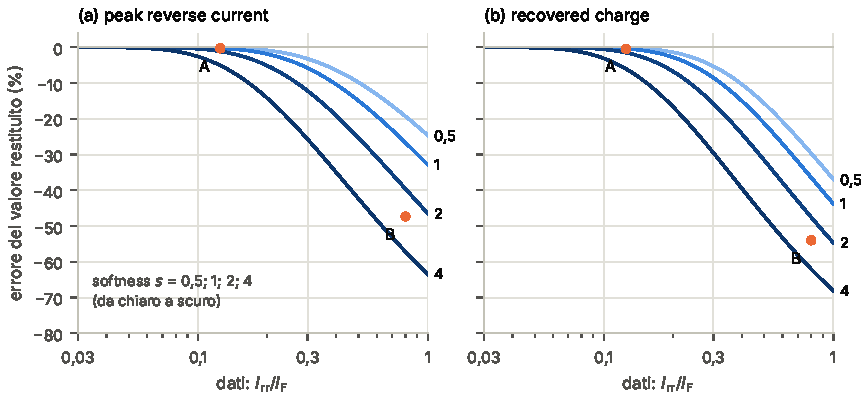
\includegraphics[width=\textwidth]{../lauritzen_ma_datasheet_conversion/figures/fig_inversion_it.pdf}
\caption{Errore della forma chiusa per rampa lunga \eqref{eq:longinv}: il set che essa fornisce è riportato sulla rampa di prova e (a) la sua corrente di picco e (b) la sua carica sono confrontate con i dati, in funzione del rapporto $\Irr/\IF$ del punto del datasheet e per quattro valori della softness. A e B sono i due esempi svolti.}
\label{fig:inversion}
\end{figure}

\subsection{Da altre coppie di dati}
\label{sec:pairs}
Il recovery ha due parametri, quindi servono due dati indipendenti in una condizione di prova. Con coppie diverse da $(\Irr, \Qrr)$ cambiano i primi due passi della Sez.~\ref{sec:invpq} e restano gli altri due.

\emph{Corrente di picco e recovery time.} Dalla \eqref{eq:trr}, con il $\kappa$ della convenzione del datasheet,
\begin{equation}
\taurr = \frac{\trr - \Irr/a}{\kappa} .
\label{eq:fromtrr}
\end{equation}
Richiede $\trr > \Irr/a$.

\emph{Carica e recovery time.} Eliminando $\taurr$ tra le \eqref{eq:qrr} e \eqref{eq:trr} si ottiene un'equazione di secondo grado nella corrente di picco, $(1-\kappa/2)\,\Irr^2 - a\,\trr\,\Irr + \kappa\,a\,\Qrr = 0$, con la soluzione
\begin{equation}
\Irr = \frac{a}{2-\kappa}\left[\trr - \sqrt{\trr^2 - \frac{2\,\kappa\,(2-\kappa)\,\Qrr}{a}}\,\right] \quad (\kappa \neq 2) , \qquad \Irr = \frac{2\,\Qrr}{\trr} \quad (\kappa = 2) .
\label{eq:fromqt}
\end{equation}
È la radice con $0 < \Irr < a\,\trr$, cioè con $\taurr > 0$. Per $\kappa \geq 1$, come in tutte le convenzioni della Tabella~\ref{tab:kappa}, esiste ed è unica se e solo se $\Qrr < a\,\trr^2/2$, cioè se la carica è minore di quella del triangolo che la rampa descriverebbe nell'intero recovery time. Poi la \eqref{eq:fromtrr} dà $\taurr$.

\emph{Un solo dato.} Con la sola carica, o il solo recovery time, la forma deve essere ipotizzata. Con una softness ipotizzata $s$, dalle \eqref{eq:qrr} e \eqref{eq:soft},
\begin{equation}
\Irr = \sqrt{\frac{2\,a\,\Qrr}{1+s}} , \qquad \taurr = \frac{s\,\Irr}{2a} .
\label{eq:fromq}
\end{equation}

\emph{Tre dati.} Quando il datasheet fornisce $\Irr$, $\Qrr$ e $\trr$, i tre sono coerenti con una tail esponenziale se $\Qrr = \Irr\,[\ta/2 + (\trr-\ta)/\kappa]$. Di solito non lo sono esattamente, perché una tail reale non è un esponenziale. La coppia $(\Irr, \Qrr)$ è allora la scelta migliore: il picco e la carica sono ciò che il circuito sente, e non dipendono da una convenzione. Il recovery time serve da verifica.

\subsection{Sensibilità ai dati}
\label{sec:sens}
I valori di datasheet hanno tolleranze, e i due valori di una coppia sono spesso massimi che non appartengono allo stesso dispositivo. Su una rampa lunga le derivate logaritmiche delle \eqref{eq:taurr} e \eqref{eq:longinv} sono
\begin{equation}
\begin{aligned}
\frac{\diff\taurr}{\taurr} &= \frac{1+s}{s}\,\frac{\diff\Qrr}{\Qrr} - \frac{2+s}{s}\,\frac{\diff\Irr}{\Irr} + \frac{1}{s}\,\frac{\diff a}{a} , \\
\frac{\diff\tau}{\tau} &= \frac{1+s}{2+s}\,\frac{\diff\Qrr}{\Qrr} - \frac{s}{2+s}\,\frac{\diff\Irr}{\Irr} - \frac{1}{2+s}\,\frac{\diff a}{a} , \\
\frac{\diff\TM}{\TM} &= \frac{\diff\tau}{\tau} + \frac{\diff\taurr}{\taurr} - \frac{\diff\Irr}{\Irr} + \frac{\diff a}{a} .
\end{aligned}
\label{eq:sens}
\end{equation}

\begin{table}[htb]
\centering\small
\caption{Variazione relativa dei parametri per una variazione relativa di un dato dell'uno per cento, su una rampa lunga, dalle \eqref{eq:sens}.}
\label{tab:sens}
\begin{tabular}{@{}lccccccccc@{}}
\toprule
 & \multicolumn{3}{c}{$s = 0,5$} & \multicolumn{3}{c}{$s = 1$} & \multicolumn{3}{c}{$s = 2$} \\
\cmidrule(lr){2-4}\cmidrule(lr){5-7}\cmidrule(l){8-10}
Dato & $\tau$ & $\taurr$ & $\TM$ & $\tau$ & $\taurr$ & $\TM$ & $\tau$ & $\taurr$ & $\TM$ \\
\midrule
$\Qrr$ & $+\lmSensTauQHalf$ & $+\lmSensTrrQHalf$ & $+\lmSensTmQHalf$ & $+\lmSensTauQOne$ & $+\lmSensTrrQOne$ & $+\lmSensTmQOne$ & $+\lmSensTauQTwo$ & $+\lmSensTrrQTwo$ & $+\lmSensTmQTwo$ \\
$\Irr$ & $-\lmSensTauIHalf$ & $-\lmSensTrrIHalf$ & $-\lmSensTmIHalf$ & $-\lmSensTauIOne$ & $-\lmSensTrrIOne$ & $-\lmSensTmIOne$ & $-\lmSensTauITwo$ & $-\lmSensTrrITwo$ & $-\lmSensTmITwo$ \\
$a$ & $-\lmSensTauAHalf$ & $+\lmSensTrrAHalf$ & $+\lmSensTmAHalf$ & $-\lmSensTauAOne$ & $+\lmSensTrrAOne$ & $+\lmSensTmAOne$ & $-\lmSensTauATwo$ & $+\lmSensTrrATwo$ & $+\lmSensTmATwo$ \\
\bottomrule
\end{tabular}
\end{table}

La Tabella~\ref{tab:sens} si legge così. Il lifetime è un risultato robusto: tutti i suoi coefficienti sono minori di uno. La tail time constant e il transit time sono fragili, tanto più quanto più il diodo è snappy: $\taurr$ è la differenza di due termini di grandezza simile, $\Qrr/\Irr$ e $\ta/2$, e per $s = 0,5$ una corrente di picco più alta dell'\SI{1}{\percent} abbassa $\TM$ del \SI{\lmSensTmIHalf}{\percent}. La softness del modello, $2\TM/\tau$, è quindi nota solo in modo approssimativo da una coppia di valori di datasheet. Quando la tensione di picco o lo smorzamento di una commutazione dipendono da essa, il transit time va verificato su una forma d'onda misurata, oppure il calcolo va ripetuto con $\TM$ ai due estremi del suo intervallo.

\subsection{Quali dati convertire}
\label{sec:which}
\begin{itemize}
\item \emph{Massimi o tipici.} Un set convertito dalle $\Qrr$ e $\Irr$ massime è il dispositivo con la carica più grande. Per lo spread tra i dispositivi di un collegamento in serie serve un secondo dispositivo con una carica più bassa. Se è nota solo la sua carica, si mantiene la softness: su una rampa lunga la \eqref{eq:long} dà $\Qrr \propto \tau^2$ e $\Irr \propto \tau$ a rapporto $\TM/\tau$ fissato, quindi un dispositivo con la carica $\Qrr'$ allo stesso di/dt ha
\begin{equation}
\tau' = \tau\,\sqrt{\Qrr'/\Qrr} , \qquad \TM' = \TM\,\sqrt{\Qrr'/\Qrr} .
\label{eq:scale}
\end{equation}
\item \emph{Temperatura.} Un set vale alla temperatura dei suoi dati. Lifetime e recovered charge crescono con la temperatura [M]~\cite{lutz}, quindi i dati alla massima temperatura di lavoro danno il recovery più grande. Tra \SI{25}{\celsius} e \SI{125}{\celsius} la recovered charge di un fast diode cresce tipicamente di un fattore attorno a due [M]~\cite{lutz}; a softness e di/dt invariati la peak reverse current cresce allora di un fattore circa $\sqrt{2}$, \eqref{eq:triangle}. Se il datasheet fornisce la carica a una seconda temperatura solo come rapporto o come curva, si applica la \eqref{eq:scale} se la rampa di prova è lunga; altrimenti si converte la nuova carica con la softness del primo punto, \eqref{eq:fromq}.
\item \emph{Punto di prova.} Se il datasheet fornisce il recovery a più di/dt, il punto da convertire è quello più vicino al di/dt dell'applicazione. La Sezione~\ref{sec:slope} spiega perché.
\end{itemize}

%=====================================================================
\section{Parametri di conduzione e del blocking state}
\label{sec:static}
\subsection{Forward characteristic}
\label{sec:forward}
Dalle \eqref{eq:static} e \eqref{eq:terminal} la caratteristica statica del modello è
\begin{equation}
v = \Nem\,\VT\,\ln\Bigl(1 + \frac{i}{\IS}\Bigr) + \RS\, i .
\label{eq:vf}
\end{equation}
Ha tre parametri. La retta \eqref{eq:line} ha due numeri, quindi un parametro va scelto, ed è l'emission coefficient $\Nem$. La retta non dà alcuna informazione su di esso: un fit della \eqref{eq:vf} su tre punti di una retta restituisce $\Nem = 0$.

\emph{Scelta di $\Nem$.} Alle sue correnti di lavoro un diodo di potenza ha la base in high injection. La concentrazione dei portatori ai bordi della base cresce allora come $e^{\vj/(2\VT)}$, dove $\vj$ è, a meno della caduta costante $\VM$, la somma delle tensioni delle due giunzioni (Sez.~\ref{sec:vf}), e poiché $\qE$ rappresenta quella concentrazione il modello richiede $\Nem = 2$. Il valore $\Nem = 1$ appartiene alla low injection, e la ricombinazione negli emitter porta la pendenza della parte di giunzione a valori intermedi; ai terminali, dove intanto sale $\VM$, la pendenza può superare $2\VT$ (Sez.~\ref{sec:emitter}). Un fit su una curva misurata può restituire altri valori ancora, perché i tre parametri assorbono allora anche ciò che il modello non ha, per esempio una resistenza della base che dipende dalla corrente.

\emph{Tangent fit.} Il modello è reso tangente alla retta a una corrente $I_0$, per esempio la forward current dell'applicazione:
\begin{equation}
\RS = \rT - \frac{\Nem\,\VT}{I_0} , \qquad \IS = \frac{I_0}{e^{(\VTo + \Nem\VT)/(\Nem\VT)} - 1} .
\label{eq:tangent}
\end{equation}
La prima relazione uguaglia le pendenze, perché la giunzione ha la resistenza incrementale $\Nem\VT/I_0$; la seconda uguaglia le tensioni, perché la junction voltage a $I_0$ è allora $\VTo + \Nem\VT$. In ogni altro punto il modello sta sotto la retta, di $\Nem\VT\,(u - 1 - \ln u)$ con $u = i/I_0$.

\emph{Secant fit.} Il modello interseca la retta alle due correnti $I_1$ e $I_2$ alle quali la retta interseca la caratteristica reale:
\begin{equation}
\RS = \rT - \frac{\Nem\,\VT\,\ln(I_2/I_1)}{I_2 - I_1} , \qquad \IS = \frac{I_1}{e^{[\VTo + (\rT-\RS)\,I_1]/(\Nem\VT)} - 1} .
\label{eq:secant}
\end{equation}
La prima relazione trascura $\IS$ rispetto a $I_1$. Entrambi i fit richiedono $\RS \geq 0$, il che limita l'emission coefficient a $\Nem \leq \rT I_0/\VT$ per la tangente e a $\Nem \leq \rT\,(I_2-I_1)/(\VT\ln(I_2/I_1))$ per la secante.

\emph{Punti di una curva.} Per $i \gg \IS$ l'equazione \eqref{eq:vf} è lineare nelle tre incognite $\Nem\VT$, $\Nem\VT\ln\IS$ e $\RS$:
\begin{equation}
v_k = \Nem\VT\,\ln i_k - \Nem\VT\,\ln\IS + \RS\, i_k .
\label{eq:points}
\end{equation}
Tre punti della forward curve danno i tre parametri con un sistema lineare, e più punti ai minimi quadrati. I punti dovrebbero coprire il campo di lavoro della corrente.

\emph{Implementazioni con $\tau\,\IS^{*}$.} Una saturation current trovata dalla caratteristica statica è la $\IS$ della \eqref{eq:qe}. Un'implementazione che scrive la junction law con $\tau\,\IS^{*}$ richiede $\IS^{*} = \IS\,(\tau+\TM)/\tau$, \eqref{eq:isstar}. Se si dimentica il fattore la forward voltage del modello è troppo alta di $\Nem\VT\ln[(\tau+\TM)/\tau]$, qualche decina di millivolt.

\subsection{Blocking state e junction capacitance}
\label{sec:blocking}
\emph{Leakage.} La resistenza $\Rr$ porta la reverse current del diodo nel blocking state: $\Rr = V/I$ alla reverse voltage e alla temperatura di interesse. Con il massimo del datasheet, $\Rr = \Vrrm/\Irrm$. Una resistenza è l'elemento più semplice che lo fa ed è corretta a una sola tensione; la reverse current di un diodo reale dipende poco dalla tensione e molto dalla temperatura [M]~\cite{lutz}. Durante il recovery il leakage è irrilevante.

\emph{Junction capacitance.} La capacità segue la convenzione di SPICE,
\begin{equation}
\Cj(\vj) = \frac{\Cjo}{(1 - \vj/\Vbi)^{m_\mathrm{j}}} \qquad \text{per } \vj < F_\mathrm{C}\,\Vbi ,
\label{eq:cj}
\end{equation}
prolungata con la sua tangente sopra $F_\mathrm{C} \Vbi$, con $\Vbi \approx \SI{0.7}{\volt}$, $m_\mathrm{j} = 0,5$ per una giunzione brusca e $F_\mathrm{C} = 0,5$. Se il datasheet fornisce la capacità $C$ a una reverse voltage $V$, allora $\Cjo = C\,(1+V/\Vbi)^{m_\mathrm{j}}$. Se non la fornisce, come accade per i grandi diodi raddrizzatori, $\Cjo$ si stima con la \eqref{eq:wsc}, che dà \SI{\pdScCjZero}{\nano\farad\per\centi\metre\squared} per $\ND = \SI{1e14}{\centi\metre^{-3}}$: il drogaggio è quello della classe di tensione (Tabella~\ref{tab:blocking}), e l'area attiva segue dalla corrente nominale con una densità dell'ordine di \SI{100}{\ampere\per\centi\metre\squared}. Non occorre che la stima sia precisa: la carica \eqref{eq:qc} è una piccola parte di $\Qrr$, e il picco \eqref{eq:vpkcj} non contiene $\Cjo$. La legge con $m_\mathrm{j} = 0,5$ vale finché la space charge region si allarga nella base: in una base punch-through, oltre la tensione a cui la space charge region raggiunge il buffer, la capacità resta quasi costante. La carica che porta la giunzione da zero alla reverse voltage $\VR$ è
\begin{equation}
Q_\mathrm{c} = \frac{\Cjo\,\Vbi}{1-m_\mathrm{j}}\left[\Bigl(1+\frac{\VR}{\Vbi}\Bigr)^{1-m_\mathrm{j}} - 1\right] .
\label{eq:qc}
\end{equation}
Questa carica scorre nel verso inverso mentre la tensione cresce, e una recovered charge misurata la comprende (Sez.~\ref{sec:rrdata}). Per un diodo di potenza è piccola rispetto alla stored charge, lo \SI{\lmAQcPct}{\percent} e lo \SI{\lmBQcPct}{\percent} di $\Qrr$ nei due esempi, quindi la conversione della Sez.~\ref{sec:inverse} può ignorarla; dove non è piccola, $Q_\mathrm{c}$ va sottratta dalla carica del datasheet prima della conversione. La capacità ha un secondo effetto: porta corrente mentre la tensione sale, quindi il picco della corrente ai terminali è un po' più alto del picco della diffusion current, e in ritardo rispetto a esso (Sez.~\ref{sec:cell}). La capacità oscilla poi con l'induttanza del circuito, già durante la tail: senza smorzamento alza la peak reverse voltage (Sez.~\ref{sec:energy}).

%=====================================================================
\section{Ciò che il modello non può riprodurre}
\label{sec:limits}
La conversione dà un set che restituisce esattamente il punto del datasheet. Lontano da quel punto il modello segue le sue leggi, e non sono quelle di un diodo reale.

\subsection{di/dt}
\label{sec:slope}
Su una rampa lunga il modello ha $\Qrr \propto a$ e $\Irr \propto a$, \eqref{eq:long}. Le curve dei datasheet di diodi raddrizzatori e tiristori sono molto più piatte: in un diagramma bilogaritmico della carica in funzione del di/dt sono vicine a rette con pendenza ben inferiore a uno (per esempio \cite{an5950}, Figg.~12 e~13). Il diodo ipotetico A ha una curva di questo tipo con l'esponente \num{\lmAQexp}. La Figura~\ref{fig:curves} e la Tabella~\ref{tab:awaya} mostrano che cosa ne segue: il set convertito a \SI{\lmASlope}{\ampere\per\micro\second} dà a \SI{\lmAAwayALo}{\ampere\per\micro\second} una carica di \SI{\lmAAwayQrrALo}{\micro\coulomb} contro i \SI{\lmAAwayDsALo}{\micro\coulomb} della curva, e a \SI{\lmAAwayAHi}{\ampere\per\micro\second} una carica \num{\lmAAwayRatioAHi} volte quella della curva.

Il motivo è che il lifetime di un diodo reale non è una costante. La ricombinazione diventa più rapida quando la concentrazione dei portatori sale, in particolare per la ricombinazione negli emitter (Sez.~\ref{sec:emitter}) \cite{schlangenotto1969}, quindi una rampa rapida, che lascia più carica nella base, incontra un lifetime efficace più breve. Un modello con $\tau$ costante non può seguirla. Il modello esteso degli stessi autori \cite{ma1993} aggiunge la ricombinazione negli emitter, al prezzo di più parametri.

Visto dal modello, ogni di/dt ha il suo set di parametri. Se una curva $\Qrr \propto a^{m}$ è convertita punto per punto su una rampa lunga con la stessa softness, la \eqref{eq:long} dà
\begin{equation}
\tau(a) = \tau(a_0)\,\Bigl(\frac{a}{a_0}\Bigr)^{-(1-m)/2} ,
\label{eq:taucurve}
\end{equation}
e la stessa legge per $\TM$. Con $m = \lmAQexp$ il lifetime scende come $a^{-\lmATauExpCurve}$: raddoppia quando il di/dt scende di un fattore sette. Le regole che ne seguono sono:
\begin{itemize}
\item convertire il punto del datasheet al di/dt più vicino a quello dell'applicazione;
\item se il datasheet fornisce una curva, leggere la carica (e la corrente di picco, se ne è data la curva) al di/dt dell'applicazione e convertire quel punto; se si legge solo la carica, mantenere la softness del punto del datasheet e usare la \eqref{eq:fromq};
\item sotto il campo della curva, come in un line-commutated converter con un di/dt di una frazione di ampere al microsecondo, non sono corretti né il modello con un set fisso né la curva estrapolata. La nota in \texttt{research/diode-stack}, Sez.~6, tratta questo caso con un termine di ricombinazione quadratico nella carica, e dà un limite inferiore e un limite superiore della carica.
\end{itemize}
Un set di parametri è una descrizione locale del diodo: è valido vicino al di/dt a cui è stato convertito. Il suo $\tau$ è il lifetime efficace di quel punto di prova, non una proprietà del materiale.

\subsection{Forward current}
Su una rampa lunga il recovery del modello non dipende affatto dalla forward current; su una rampa corta cresce con essa, e gli esponenti rispetto al di/dt e rispetto alla forward current sommano a uno, \eqref{eq:euler}. È una verifica che si può fare su un datasheet prima di qualunque conversione: se le sue curve in funzione del di/dt e della forward current hanno esponenti che non sommano a uno vicino al punto di lavoro, nessun set di parametri riproduce entrambe. Il set va allora convertito anche alla forward current dell'applicazione.

\subsection{Reverse voltage, temperatura, forward recovery, tail}
\label{sec:otherlimits}
\begin{itemize}
\item \emph{Reverse voltage.} La tail \eqref{eq:tail} non dipende dalla tensione ai capi del diodo, come osservano gli autori per la propria implementazione \cite{pemodels}. Un set convertito alla reverse voltage della prova del datasheet si usa invariato a un'altra tensione. In un diodo reale la corrente di picco e la carica dipendono poco dalla tensione, e la softness può dipenderne molto di più [M]~\cite{lutz}.
\item \emph{Temperatura.} Le equazioni contengono la temperatura solo in $\VT$. I parametri del recovery valgono alla temperatura dei dati (Sez.~\ref{sec:which}).
\item \emph{Forward recovery.} Il modello ha una resistenza serie costante: non ha overshoot di tensione al turn-on. Il modello esteso \cite{ma1993} aggiunge la conductivity modulation della base.
\item \emph{Forma della tail.} La tail del modello è sempre un solo esponenziale. Una tail reale può avere due pendenze o terminare bruscamente, e allora la terna $\Irr$, $\Qrr$, $\trr$ del datasheet non è coerente con la \eqref{eq:trr}.
\end{itemize}

%=====================================================================
\section{Altri set di parametri e simulatori}
\label{sec:others}
La Tabella~\ref{tab:others} mette in relazione i parametri $\tau$ e $\TM$ del modello a due cariche con quelli di altre implementazioni e di altri due modelli di diodo.

\begin{table}[htb]
\centering\small
\caption{I parametri del recovery in altre implementazioni e modelli.}
\label{tab:others}
\begin{tabular}{@{}>{\raggedright\arraybackslash}p{4.6cm}>{\raggedright\arraybackslash}p{4.2cm}>{\raggedright\arraybackslash}p{7.2cm}@{}}
\toprule
Modello o implementazione & Parametri del recovery & Relazione con $\tau$ e $\TM$ \\
\midrule
Componente di libreria \texttt{diode\_rr} (libreria pwr-control) & \texttt{tau}, \texttt{TM} & gli stessi; junction law con $\tau\,\IS^{*}$, quindi $\IS^{*} = \IS(\tau+\TM)/\tau$, \eqref{eq:isstar} \\
\addlinespace
Blocco diodo con dinamica di carica \cite{mathworks} & carrier lifetime e transit time, oppure $\Irr$ e $a$ con uno tra $\trr$, stretch factor, $\Qrr$ & transit time $= \TM$; $\trr$ con la convenzione del \SI{10}{\percent}; la documentazione riporta la soluzione su rampa della Sez.~\ref{sec:ramp} e dichiara che la condizione di picco è risolta per iterazione \\
\addlinespace
Forma SPICE sulle pagine web degli autori del modello \cite{pemodels} & \texttt{Tau}, \texttt{TT} & $\texttt{Tau} = \tau$, $\texttt{TT} = \TM$; ``conversioni approssimate'' $\Qrr = \texttt{Tau}\cdot\IF$ e $1/\trr = 1/\texttt{Tau} + 1/\texttt{TT}$ \\
\addlinespace
Diodo di SPICE & \texttt{TT} & una sola carica, pari a $\texttt{TT}$ per la corrente statica: $\tau = \texttt{TT}$ e $\TM = 0$, quindi $s = 0$ \\
\addlinespace
Behavioural diode con reverse recovery \cite{plecs} & due tra $\trr$, $\Irr$, $\Qrr$, con la forward current e il di/dt della prova & non è un modello di carica: i valori del datasheet sono inseriti così come sono; $\trr$ con la convenzione del \SI{10}{\percent} \\
\bottomrule
\end{tabular}
\end{table}

\emph{Le conversioni approssimate.} Le due relazioni citate nella terza riga sono il limite di commutazione brusca della Sez.~\ref{sec:limitsramp}. Con $\taurr \ll \tau$, la \eqref{eq:abrupt} è $\Qrr = \tau\IF$, e dopo una commutazione brusca il recovery dura circa una tail time constant, $1/\taurr = 1/\tau + 1/\TM$. Valgono per un diodo commutato molto più rapidamente del suo lifetime. Per un diodo provato su una rampa sono molto lontane: per il diodo A, $\tau\IF$ è \num{\lmATauIfRatio} volte la recovered charge del datasheet, e un lifetime letto come $\Qrr/\IF$ sarebbe \SI{\lmAQoverIf}{\micro\second} invece di \SI{\lmATau}{\micro\second}.

\emph{Il diodo di SPICE.} Il suo unico parametro di storage è il transit time \texttt{TT}, e la sua stored charge è \texttt{TT} per la corrente statica alla junction voltage attuale [M]~\cite{nagel1975}. La carica obbedisce allora alla prima delle \eqref{eq:conducting} con $\tau = \texttt{TT}$ e non c'è un'edge charge separata: è il modello a controllo di carica della Sez.~\ref{sec:chargecontrol}, cioè il modello a due cariche con $\TM = 0$. La reverse current termina bruscamente quando la carica è esaurita. Il nome è una trappola: il \texttt{TT} di SPICE ha il ruolo del lifetime $\tau$, mentre il \texttt{TT} delle implementazioni del modello di Lauritzen--Ma è $\TM$.

\emph{Behavioural model.} Un behavioural model prende direttamente i valori del datasheet e con essi dà forma a un generatore di corrente; non richiede conversione, ma non sa come il recovery cambia con il di/dt e con la forward current. Per alimentare un tale modello con il recovery time di un set $\tau$, $\TM$, la \eqref{eq:trr} con $\kappa = \lmKTen$ dà il valore nella sua convenzione.

%=====================================================================
\section{Esempi svolti}
\label{sec:examples}
\subsection{Dati}
Si ipotizzano i due diodi della Tabella~\ref{tab:data}. Il diodo A è un diodo raddrizzatore per frequenza di rete con un'alta blocking voltage, provato su una rampa lenta; il diodo B è un fast diode del tipo usato come freewheeling diode in uno switching leg, provato su una rampa rapida. Sono stati scelti per stare ai due estremi della Fig.~\ref{fig:map}: A su una rampa lunga e B su una corta.

\begin{table}[htb]
\centering\small
\caption{Datasheet ipotetici dei due esempi.}
\label{tab:data}
\begin{tabular}{@{}lll@{}}
\toprule
 & Diodo A, diodo raddrizzatore & Diodo B, fast diode \\
\midrule
Repetitive peak reverse voltage $\Vrrm$ & \SI{\lmAVrrm}{\volt} & \SI{\lmBVrrm}{\volt} \\
Reverse current a $\Vrrm$, massima & \SI{\lmAIrrmMa}{\milli\ampere} & \SI{\lmBIrrmMa}{\milli\ampere} \\
Temperatura di giunzione dei dati & \SI{\lmAT}{\celsius} & \SI{\lmBT}{\celsius} \\
Forward characteristic & $\VTo = \SI{\lmAVto}{\volt}$, $\rT = \SI{\lmARt}{\milli\ohm}$, & \SI{\lmBVfOne}{\volt} a \SI{\lmBIfOne}{\ampere}, \SI{\lmBVfTwo}{\volt} a \SI{\lmBIfTwo}{\ampere}, \\
 & retta per \SI{\lmAIone}{\ampere} e \SI{\lmAItwo}{\ampere} & \SI{\lmBVfThree}{\volt} a \SI{\lmBIfThree}{\ampere} \\
Prova di recovery: forward current $\IF$ & \SI{\lmAIf}{\ampere} & \SI{\lmBIf}{\ampere} \\
Prova di recovery: di/dt $a$ & \SI{\lmASlope}{\ampere\per\micro\second} & \SI{\lmBSlope}{\ampere\per\micro\second} \\
Prova di recovery: reverse voltage $\VR$ & \SI{\lmAVr}{\volt} & \SI{\lmBVr}{\volt} \\
Peak reverse recovery current $\Irr$ & \SI{\lmAIrr}{\ampere} (massima) & \SI{\lmBIrr}{\ampere} (tipica) \\
Recovered charge $\Qrr$ & \SI{\lmAQrr}{\micro\coulomb} (massima) & \SI{\lmBQrr}{\micro\coulomb} (tipica) \\
Carica in funzione del di/dt & $\Qrr \propto a^{\lmAQexp}$ per \SIrange{\lmAQrangeLo}{\lmAQrangeHi}{\ampere\per\micro\second} & non data \\
Seconda temperatura & non data & \SI{\lmBTtwo}{\celsius}: $\Irr = \SI{\lmBIrrTtwo}{\ampere}$, $\Qrr = \SI{\lmBQrrTtwo}{\micro\coulomb}$ \\
\bottomrule
\end{tabular}
\end{table}

\subsection{Parametri del recovery}
\label{sec:exrec}
La Tabella~\ref{tab:conv} segue i quattro passi della Sez.~\ref{sec:invpq} e aggiunge la forma chiusa per confronto.

\begin{table}[htb]
\centering\small
\caption{Conversione dei dati di recovery.}
\label{tab:conv}
\begin{tabular}{@{}llcc@{}}
\toprule
Grandezza & & Diodo A & Diodo B \\
\midrule
Rapporto $\Irr/\IF$ dei dati & & \lmAIrrOverIf & \lmBIrrOverIf \\
Tempo al picco $\ta = \Irr/a$ & & \SI{\lmATa}{\micro\second} & \SI{\lmBTa}{\nano\second} \\
Carica del triangolo, $\Irr\ta/2$ & & \SI{\lmAQtri}{\micro\coulomb} (\SI{\lmAQtriPct}{\percent} di $\Qrr$) & \SI{\lmBQtri}{\micro\coulomb} (\SI{\lmBQtriPct}{\percent}) \\
Tail time constant $\taurr$ & \eqref{eq:taurr} & \SI{\lmATrr}{\micro\second} & \SI{\lmBTrr}{\nano\second} \\
Softness dei dati, $s = 2\taurr/\ta$ & \eqref{eq:soft} & \lmAS & \lmBS \\
\addlinespace
Forma chiusa: $\tau$, $\TM$ & \eqref{eq:longinv} & \SI{\lmATauL}{\micro\second}, \SI{\lmATmL}{\micro\second} & \SI{\lmBTauL}{\nano\second}, \SI{\lmBTmL}{\nano\second} \\
Esatti: $\tau$, $\TM$ & \eqref{eq:iter}, \eqref{eq:tm} & \SI{\lmATau}{\micro\second}, \SI{\lmATm}{\micro\second} & \SI{\lmBTau}{\nano\second}, \SI{\lmBTm}{\nano\second} \\
Iterazioni della \eqref{eq:iter} fino a $10^{-13}$ & & \lmAIter & \lmBIter \\
Errore della forma chiusa su $\tau$, $\TM$ & & $\lmATauLErr\,\%$, $\lmATmLErr\,\%$ & $\lmBTauLErr\,\%$, $\lmBTmLErr\,\%$ \\
Set della forma chiusa sulla rampa di prova: $\Irr$ & & \SI{\lmAIrrBackL}{\ampere} ($\lmAIrrBackLErr\,\%$) & \SI{\lmBIrrBackL}{\ampere} ($\lmBIrrBackLErr\,\%$) \\
Set della forma chiusa sulla rampa di prova: $\Qrr$ & & \SI{\lmAQrrBackL}{\micro\coulomb} ($\lmAQrrBackLErr\,\%$) & \SI{\lmBQrrBackL}{\micro\coulomb} ($\lmBQrrBackLErr\,\%$) \\
\addlinespace
$\rho = \taurr/\tau$; $\TM/\tau$ & \eqref{eq:rho} & \lmARho; \lmATmOverTau & \lmBRho; \lmBTmOverTau \\
$\lambda = \IF/(a\tau)$ & \eqref{eq:normdef} & \lmALam & \lmBLam \\
Durata della rampa, $\xi = \Tone/\tau$ & & \lmAX & \lmBX \\
Fattore $1-e^{-\xi}$ & \eqref{eq:peak} & \lmAF & \lmBF \\
Softness su rampa lunga, $2\TM/\tau$ & \eqref{eq:softlong} & \lmASoftLong & \lmBSoftLong \\
\addlinespace
Carica allo zero della corrente & \eqref{eq:qzero} & \SI{\lmAQzero}{\micro\coulomb} & \SI{\lmBQzero}{\micro\coulomb} \\
Carica statica $\tau\IF$ & \eqref{eq:static} & \SI{\lmAQstat}{\micro\coulomb} & \SI{\lmBQstat}{\micro\coulomb} \\
$\Qrr$ rispetto alla carica allo zero della corrente & & \SI{\lmAQzeroPct}{\percent} & \SI{\lmBQzeroPct}{\percent} \\
Esponenti di $\Irr$ rispetto ad $a$ e $\IF$ & \eqref{eq:exponents} & \lmAExpIa; \lmAExpIf & \lmBExpIa; \lmBExpIf \\
Esponenti di $\Qrr$ rispetto ad $a$ e $\IF$ & \eqref{eq:exponents} & \lmAExpQa; \lmAExpQf & \lmBExpQa; \lmBExpQf \\
\bottomrule
\end{tabular}
\end{table}

\emph{Diodo A.} La peak reverse current è un ottavo della forward current, e la rampa dalla forward current al picco dura \SI{\lmATone}{\micro\second}, cioè \num{\lmAX} lifetime: una rampa lunga. La forma chiusa è corretta entro mezzo punto percentuale, e la forward current della prova non ha alcuna influenza. Quando la corrente attraversa lo zero la base contiene \SI{\lmAQzero}{\micro\coulomb}, un quinto della carica statica; il \SI{\lmAQzeroPct}{\percent} di essa esce come recovered charge, come dice la \eqref{eq:fraction} per $\rho = \lmARho$.

\emph{Diodo B.} La peak reverse current è l'\SI{80}{\percent} della forward current, e la rampa dura \SI{\lmBTone}{\nano\second}, cioè \num{\lmBX} lifetime: una rampa corta. Allo zero della corrente la base contiene ancora la maggior parte della sua carica statica. La forma chiusa dà un lifetime più corto di un terzo e un transit time più lungo del \SI{43}{\percent}, e quel set, riportato sulla rampa di prova, restituisce circa metà della corrente di picco e della carica del datasheet. Il set esatto richiede \lmBIter{} iterazioni perché il rapporto $\Irr/(\IF+\Irr)$ è grande. La softness dei dati è \num{\lmBS}, ma solo \num{\lmBSoftLong} appartiene al diodo e il resto alla rampa corta: su una rampa lenta lo stesso diodo apparirebbe molto meno soft. Il recovery dipende dalla forward current più che dal di/dt.

In entrambi i casi il set esatto restituisce il punto del datasheet: la forma chiusa \eqref{eq:lambert} e un'integrazione passo passo delle \eqref{eq:idif} e \eqref{eq:qm} concordano su $\Irr$ e $\Qrr$ entro $10^{-8}$.

\emph{Verifica dell'ordine di grandezza.} Il transit time si può confrontare con la larghezza di base che la classe di tensione richiede (Sez.~\ref{sec:onenumber}). Con un'ambipolar diffusion constant di \SI{\lmADcm}{\centi\metre\squared\per\second}, un valore indicativo per il silicio a \SI{\lmAT}{\celsius} [M]~\cite{lutz}, il transit time del diodo A corrisponde a una larghezza di base di \SI{\lmAWpar}{\micro\metre} con la \eqref{eq:tmgeom}, \SI{\lmAWmode}{\micro\metre} con la \eqref{eq:tmtail} a mobilità uguali e \SI{\lmAWstat}{\micro\metre} con la \eqref{eq:tmstatic}; con il rapporto delle mobilità del silicio, \SI{\pdAWblock}{\micro\metre} con la \eqref{eq:tmasym} e \SI{\pdAWtail}{\micro\metre} con la \eqref{eq:tmtail}. Per il diodo B, con \SI{\lmBDcm}{\centi\metre\squared\per\second}, le stesse relazioni danno \SI{\lmBWpar}{\micro\metre}, \SI{\lmBWmode}{\micro\metre} e \SI{\lmBWstat}{\micro\metre}, e poi \SI{\pdBWblock}{\micro\metre} e \SI{\pdBWtail}{\micro\metre}. Le due diffusion constant sono quelle della nota sul modello di Lauritzen--Ma; le leggi di potenza della Sez.~\ref{sec:ambipolar} danno valori di poco inferiori, e le larghezze scendono di circa il \SI{\pdAWlawPct}{\percent}. Le cinque stime coprono un fattore due: la verifica distingue un transit time plausibile da uno lontano di un ordine di grandezza, non di più.

Per il diodo A si può fare un passo oltre, perché la sua base non è sottile: la diffusion length è \SI{\lmALdiff}{\micro\metre}, una base da \SI{\lmAVrrmKv}{\kilo\volt} è larga circa mezzo millimetro (Tabella~\ref{tab:blocking}), e la softness \num{\lmAS} su una rampa lunga è quella di una base larga (Tabella~\ref{tab:distributed}). La base distribuita con emitter ideali che riproduce sia il picco sia la carica del datasheet ha $d/\La = \num{\pdADistBeta}$ e $\tau = \SI{\pdADistTau}{\micro\second}$, cioè una larghezza di \SI{\pdADistW}{\micro\metre}. Ma a pari picco ogni base con $d/\La$ sopra \num{\pdADistLoBeta}, cioè più larga di circa \SI{\pdADistLoWmm}{\milli\metre}, dà la carica entro il \SI{\pdADistTol}{\percent}, e una seconda soluzione esatta è a \SI{\pdADistWmmHi}{\milli\metre}. I dati di recovery fissano quindi un limite inferiore della larghezza, coerente con la classe di tensione, e un lifetime tra \SI{\pdADistTauLo}{\micro\second} e \SI{\pdADistTauInf}{\micro\second}, contro i \SI{\lmATau}{\micro\second} della conversione: è la differenza che la Tabella~\ref{tab:distributed} prevede per una base larga.

Per il diodo B le cinque stime stanno tutte sotto i circa \SI{\pdSiUniW}{\micro\metre} di una base da \SI{\lmBVrrmKv}{\kilo\volt}: valgono da poco più della metà a meno di un terzo di quella larghezza. La base distribuita non offre una via d'uscita: la softness dei dati è \num{\lmBS}, mentre allo stesso rapporto $\Irr/\IF$ una base distribuita con emitter ideali e lifetime costante non supera \num{\pdBDistSmax}. Una tail così lunga viene da ciò che il modello non contiene, cioè dalle tecnologie della Sez.~\ref{sec:technology} che tengono plasma dal lato del catodo. I due parametri sono allora \emph{behavioural}: riproducono la forma d'onda di prova, non l'interno del dispositivo. I dati di entrambi i diodi sono ipotetici, quindi questi numeri non dicono nulla su componenti reali; mostrano come si legge la verifica.

\subsection{Parametri di conduzione e del blocking state}
\emph{Diodo A.} La thermal voltage a \SI{\lmAT}{\celsius} è \SI{\lmAVt}{\milli\volt}. Con $\Nem = \lmAN$ il secant fit \eqref{eq:secant} per \SI{\lmAIone}{\ampere} e \SI{\lmAItwo}{\ampere} dà $\RS = \SI{\lmARsSecTwo}{\milli\ohm}$ e $\IS = \lmAIsSecTwo\,\mathrm{A}$; il tangent fit \eqref{eq:tangent} a \SI{\lmAIf}{\ampere} dà $\RS = \SI{\lmARsTanTwo}{\milli\ohm}$ e $\IS = \lmAIsTanTwo\,\mathrm{A}$. Con $\Nem = 1$ il secant fit dà $\RS = \SI{\lmARsSecOne}{\milli\ohm}$ e $\IS = \lmAIsSecOne\,\mathrm{A}$. La Figura~\ref{fig:forward}a mostra che la scelta di $\Nem$ non conta all'interno del campo della retta e conta al di sotto: a \SI{100}{\ampere} il modello con $\Nem = 2$ dà \SI{\lmAVlow}{\volt} e con $\Nem = 1$ \SI{\lmAVlowOne}{\volt}, contro gli \SI{\lmAVlowLine}{\volt} della retta. Il limite di $\Nem$ per una $\RS$ positiva è \num{\lmANmaxSec}, molto lontano. Un'implementazione con $\tau\,\IS^{*}$ richiede $\IS^{*} = \lmAIsFactor\,\IS = \lmAIsStar\,\mathrm{A}$; senza il fattore la forward voltage sarebbe troppo alta di \SI{\lmAIsOffsetMv}{\milli\volt}. La leakage resistance è $\Rr = \Vrrm/\Irrm = \SI{\lmARr}{\kilo\ohm}$.

\emph{Diodo B.} I tre punti della forward curve danno, con la \eqref{eq:points} e $\VT = \SI{\lmBVt}{\milli\volt}$, $\Nem = \lmBN$, $\RS = \SI{\lmBRs}{\milli\ohm}$ e $\IS = \lmBIs\,\mathrm{A}$ (Fig.~\ref{fig:forward}b). Per confronto, la retta per i due punti superiori ha $\VTo = \SI{\lmBVto}{\volt}$ e $\rT = \SI{\lmBRt}{\milli\ohm}$. Qui $\IS^{*} = \lmBIsFactor\,\IS = \lmBIsStar\,\mathrm{A}$, e $\Rr = \SI{\lmBRr}{\mega\ohm}$.

\begin{figure}[htb]
\centering
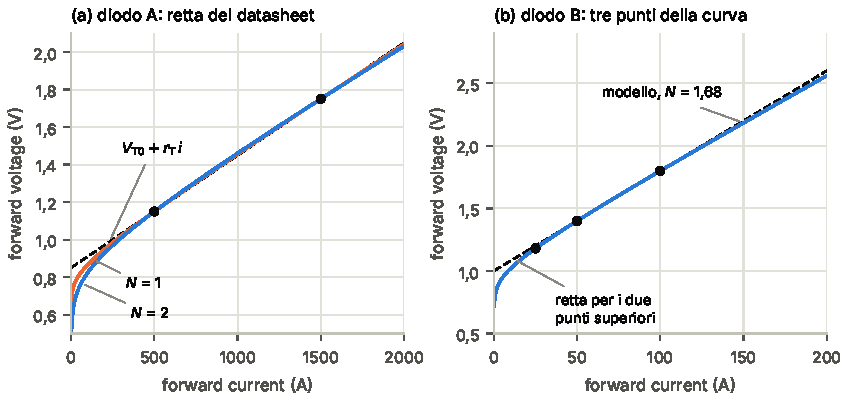
\includegraphics[width=\textwidth]{figures/fig_forward_it.pdf}
\caption{Forward characteristic del modello confrontata con i dati. (a) Diodo A: retta del datasheet (tratteggiata), con i suoi due punti, e il secant fit per $\Nem = 1$ e $\Nem = 2$. (b) Diodo B: fit su tre punti della curva, e la retta per i due punti superiori (tratteggiata).}
\label{fig:forward}
\end{figure}

\subsection{Verifica in una commutation cell simulata}
\label{sec:cell}
Il modello completo, con la junction capacitance, il leakage e la resistenza serie, è stato simulato nella cella della Fig.~\ref{fig:commcell}a con $\Ls = \VR/a$ e uno snubber RC (Appendice~\ref{app:scripts}). Le junction capacitance sono stime, $\Cjo = \SI{\lmACj}{\nano\farad}$ per A e \SI{\lmBCj}{\nano\farad} per B. La Tabella~\ref{tab:cell} confronta la simulazione con le forme chiuse e la Figura~\ref{fig:cell} mostra le forme d'onda.

\begin{table}[htb]
\centering\small
\caption{Commutation cell simulata confrontata con le forme chiuse. Le forme chiuse sono valutate al di/dt della simulazione; la carica è integrata fino al \SI{\lmPEndPct}{\percent} del picco, \eqref{eq:qrp}.}
\label{tab:cell}
\begin{tabular}{@{}lcc@{}}
\toprule
 & Diodo A & Diodo B \\
\midrule
Induttanza $\Ls = \VR/a$ & \SI{\lmAL}{\micro\henry} & \SI{\lmBL}{\micro\henry} \\
Snubber $\Rsn$, $\Csn$ & \SI{\lmARsn}{\ohm}, \SI{\lmACsn}{\nano\farad} & \SI{\lmBRsn}{\ohm}, \SI{\lmBCsn}{\nano\farad} \\
di/dt allo zero della corrente & \SI{\lmASimSlope}{\ampere\per\micro\second} ($\lmASimSlopeErr\,\%$) & \SI{\lmBSimSlope}{\ampere\per\micro\second} ($\lmBSimSlopeErr\,\%$) \\
\addlinespace
$\Irr$, forma chiusa \eqref{eq:lambert} & \SI{\lmASimIrrCf}{\ampere} & \SI{\lmBSimIrrCf}{\ampere} \\
$\Irr$, simulazione, diffusion current & \SI{\lmASimIrrDif}{\ampere} ($\lmASimIrrDifErr\,\%$) & \SI{\lmBSimIrrDif}{\ampere} ($\lmBSimIrrDifErr\,\%$) \\
$\Irr$, simulazione, ai terminali & \SI{\lmASimIrrTerm}{\ampere} ($\lmASimIrrTermErr\,\%$) & \SI{\lmBSimIrrTerm}{\ampere} ($\lmBSimIrrTermErr\,\%$) \\
\addlinespace
$Q_\mathrm{r}$, forma chiusa \eqref{eq:qrp} & \SI{\lmASimQCf}{\micro\coulomb} & \SI{\lmBSimQCf}{\micro\coulomb} \\
$Q_\mathrm{r}$, simulazione, ai terminali & \SI{\lmASimQTerm}{\micro\coulomb} ($\lmASimQTermErr\,\%$) & \SI{\lmBSimQTerm}{\micro\coulomb} ($\lmBSimQTermErr\,\%$) \\
Carica della junction capacitance, \eqref{eq:qc} & \SI{\lmAQc}{\micro\coulomb} & \SI{\lmBQc}{\micro\coulomb} \\
\addlinespace
$\trr$, retta, forma chiusa \eqref{eq:trr} & \SI{\lmASimTrrCf}{\micro\second} & \SI{\lmBSimTrrCf}{\nano\second} \\
$\trr$, retta, simulazione & \SI{\lmASimTrr}{\micro\second} & \SI{\lmBSimTrr}{\nano\second} \\
\addlinespace
Peak reverse voltage senza capacità, \eqref{eq:vrm} & \SI{\lmAVpk}{\volt} & \SI{\lmBVpk}{\volt} \\
\quad con la sola junction capacitance, \eqref{eq:vpkcj} & \SI{\pdAVpkCj}{\volt} & \SI{\pdBVpkCj}{\volt} \\
\quad con la sola junction capacitance, simulazione & \SI{\pdAVpkCjSim}{\volt} & \SI{\pdBVpkCjSim}{\volt} \\
\quad con lo snubber, simulazione & \SI{\lmASimVpk}{\volt} & \SI{\lmBSimVpk}{\volt} \\
Energia nel diodo dopo lo zero della corrente & \SI{\lmASimEd}{\milli\joule} & \SI{\lmBSimEd}{\milli\joule} \\
Energia nel resistore dello snubber & \SI{\lmASimEr}{\milli\joule} & \SI{\lmBSimEr}{\milli\joule} \\
Somma & \SI{\lmASimEsum}{\milli\joule} & \SI{\lmBSimEsum}{\milli\joule} \\
Bilancio $\VR\Qrr + \Csn\VR^2/2$, \eqref{eq:ebal} & \SI{\lmASimEbal}{\milli\joule} & \SI{\lmBSimEbal}{\milli\joule} \\
\bottomrule
\end{tabular}
\end{table}

La tabella mostra quattro cose.
\begin{itemize}
\item Il di/dt allo zero della corrente è un po' sopra $\VR/\Ls$, perché la forward voltage del diodo si somma a $\VR$ mentre la corrente scende. L'effetto è qui inferiore all'uno per cento; cresce quando $\VR$ è piccola.
\item La diffusion current della simulazione segue la forma chiusa entro lo \SI{0.5}{\percent}. La corrente ai terminali è più alta al picco, dello \SI{0.1}{\percent} per A e dell'\SI{1.5}{\percent} per B: è la corrente della junction capacitance mentre la tensione sale. Per il diodo B la carica ai terminali supera la forma chiusa dello \SI{0.3}{\percent}, che è la carica della junction capacitance, come dice la nota della norma. Per il diodo A quella carica è trascurabile, e lo \SI{0.1}{\percent} che resta viene dal di/dt, che non è esattamente costante lungo la rampa perché la forward voltage cambia con la corrente.
\item Il recovery time della convenzione della retta è riprodotto entro lo \SI{0.6}{\percent}.
\item Il bilancio dell'energia \eqref{eq:ebal} si chiude entro lo \SI{0.5}{\percent}. Senza lo snubber la sola junction capacitance porterebbe il picco della tensione a circa \SI{\pdAVpkCjSim}{\volt} per A e \SI{\pdBVpkCjSim}{\volt} per B, come prevede la \eqref{eq:vpkcj}: per il diodo B molto oltre la sua $\Vrrm$ di \SI{\lmBVrrm}{\volt}. Lo snubber smorza questa oscillazione. Per il diodo A è rapido rispetto alla tail ($\Rsn\Csn = \SI{\lmARsnCsn}{\micro\second}$, $\taurr = \SI{\lmATrr}{\micro\second}$): il picco è \SI{\lmASimVpk}{\volt}, praticamente i \SI{\lmAVpk}{\volt} che la \eqref{eq:vrm} dà senza capacità, e quasi tutta l'energia resta nel diodo. Per il diodo B è lento quanto la tail ($\Rsn\Csn = \SI{\lmBRsnCsn}{\nano\second}$, $\taurr = \SI{\lmBTrr}{\nano\second}$): porta il picco a \SI{\lmBSimVpk}{\volt}, sotto i \SI{\lmBVpk}{\volt} della \eqref{eq:vrm}, e prende più di metà dell'energia.
\end{itemize}

\begin{figure}[htb]
\centering
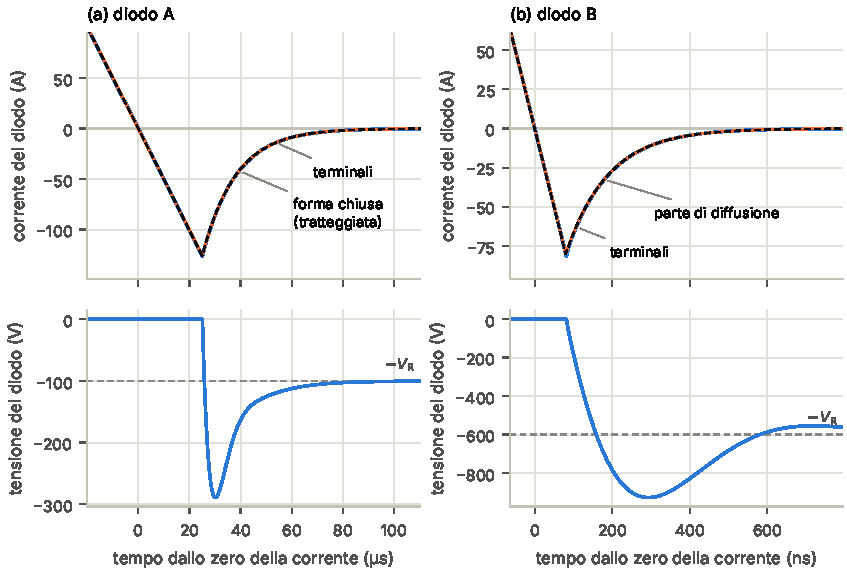
\includegraphics[width=\textwidth]{../lauritzen_ma_datasheet_conversion/figures/fig_cell_it.pdf}
\caption{Commutation cell simulata con lo snubber: corrente e tensione del diodo. La corrente ai terminali, la diffusion current e la forma chiusa della Sez.~\ref{sec:ramp} (tratteggiata) si sovrappongono; per il diodo B, al picco, la corrente ai terminali supera di poco la diffusion current (nella figura ``parte di diffusione''): la differenza è la corrente della junction capacitance.}
\label{fig:cell}
\end{figure}

\subsection{Lontano dal punto del datasheet}
\label{sec:away}
La Tabella~\ref{tab:awaya} e la Figura~\ref{fig:curves} mostrano i due set ad altri di/dt e forward current.

\begin{table}[htb]
\centering\small
\caption{Diodo A lontano dal punto del datasheet, a $\IF = \SI{\lmAIf}{\ampere}$: il set della Tabella~\ref{tab:conv} confrontato con la curva ipotetica del datasheet, e il set che la curva richiede a ogni di/dt (punto della curva convertito con la softness del punto del datasheet).}
\label{tab:awaya}
\begin{tabular}{@{}lccccc@{}}
\toprule
di/dt $a$ [\si{\ampere\per\micro\second}] & \lmAAwayALo & \lmAAwayALoB & \lmAAwayARef & \lmAAwayAHiB & \lmAAwayAHi \\
\midrule
Durata della rampa, $\xi = \Tone/\tau$ & \lmAAwayXALo & \lmAAwayXALoB & \lmAAwayXARef & \lmAAwayXAHiB & \lmAAwayXAHi \\
$\Irr$ del set [A] & \lmAAwayIrrALo & \lmAAwayIrrALoB & \lmAAwayIrrARef & \lmAAwayIrrAHiB & \lmAAwayIrrAHi \\
$\Qrr$ del set [\si{\micro\coulomb}] & \num{\lmAAwayQrrALo} & \num{\lmAAwayQrrALoB} & \num{\lmAAwayQrrARef} & \num{\lmAAwayQrrAHiB} & \num{\lmAAwayQrrAHi} \\
$\Qrr$ della curva del datasheet [\si{\micro\coulomb}] & \lmAAwayDsALo & \lmAAwayDsALoB & \lmAAwayDsARef & \lmAAwayDsAHiB & \lmAAwayDsAHi \\
Set rispetto alla curva & \lmAAwayRatioALo & \lmAAwayRatioALoB & \lmAAwayRatioARef & \lmAAwayRatioAHiB & \lmAAwayRatioAHi \\
\addlinespace
Punto della curva convertito: $\tau$ [\si{\micro\second}] & \lmAAwayTauALo & \lmAAwayTauALoB & \lmAAwayTauARef & \lmAAwayTauAHiB & \lmAAwayTauAHi \\
Punto della curva convertito: $\TM$ [\si{\micro\second}] & \lmAAwayTmALo & \lmAAwayTmALoB & \lmAAwayTmARef & \lmAAwayTmAHiB & \lmAAwayTmAHi \\
\bottomrule
\end{tabular}
\end{table}

Per il diodo A la rampa del set dura almeno cinque lifetime fino a \SI{\pdALongSlopeFive}{\ampere\per\micro\second} e tre fino a \SI{\pdALongSlopeThree}{\ampere\per\micro\second}; a \SI{10}{\ampere\per\micro\second} dura \num{\lmAAwayXAHiB} lifetime, e le relazioni per rampa lunga sbagliano del \SI{\pdATenIrrPct}{\percent} sul picco e del \SI{\pdATenQrrPct}{\percent} sulla carica. Fino a lì la carica del set è proporzionale al di/dt, mentre la curva del datasheet cresce con l'esponente \num{\lmAQexp}. Una decade sotto il punto del datasheet il set ha un quinto della carica della curva. Le ultime due righe sono i set che riproducono la curva a ogni di/dt: il lifetime va da \SI{\lmAAwayTauALo}{\micro\second} al di/dt più basso a \SI{\lmAAwayTauAHi}{\micro\second} al più alto, seguendo la \eqref{eq:taucurve} finché la rampa è lunga. Al di/dt del datasheet la forward current non ha quasi effetto: \SI{\lmAAwayQrrFLo}{\micro\coulomb} a \SI{\lmAAwayFLo}{\ampere} e \SI{\lmAAwayQrrFHi}{\micro\coulomb} a \SI{\lmAAwayFHi}{\ampere}, contro \SI{\lmAQrr}{\micro\coulomb} a \SI{\lmAIf}{\ampere}.

Il diodo B si comporta in modo opposto. A di/dt doppio la carica cresce da \SI{\lmBQrr}{\micro\coulomb} a soli \SI{\lmBAwayQrrAHi}{\micro\coulomb}, e a metà di/dt scende a \SI{\lmBAwayQrrALo}{\micro\coulomb}; a forward current doppia è \SI{\lmBAwayQrrFHi}{\micro\coulomb} e a metà forward current \SI{\lmBAwayQrrFLo}{\micro\coulomb}. La corrente di picco va da \SI{\lmBAwayIrrALo}{\ampere} a \SI{\lmBAwayIrrAHi}{\ampere} sui due di/dt e da \SI{\lmBAwayIrrFLo}{\ampere} a \SI{\lmBAwayIrrFHi}{\ampere} sulle due correnti. Il punto a metà di/dt e il punto a forward current doppia hanno lo stesso rapporto $\IF/a$, e il secondo vale il doppio del primo, nel picco e nella carica: è l'omogeneità della Sez.~\ref{sec:exponents}.

\begin{figure}[htb]
\centering
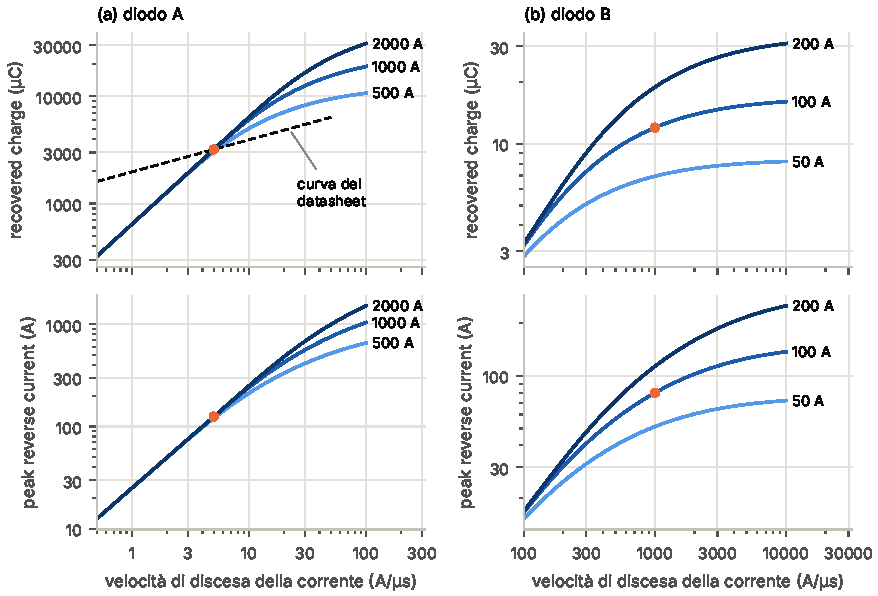
\includegraphics[width=\textwidth]{../lauritzen_ma_datasheet_conversion/figures/fig_curves_it.pdf}
\caption{I due set della Tabella~\ref{tab:conv} ad altri di/dt, per metà, una e due volte la forward current della prova del datasheet. Il punto è il punto del datasheet. Per il diodo A la linea tratteggiata è la curva ipotetica del datasheet.}
\label{fig:curves}
\end{figure}

\subsection{Temperatura}
Per il diodo B il datasheet fornisce il recovery anche a \SI{\lmBTtwo}{\celsius}. La stessa conversione dà $\taurr = \SI{\lmBTrrTtwo}{\nano\second}$, $\tau = \SI{\lmBTauTtwo}{\nano\second}$ e $\TM = \SI{\lmBTmTtwo}{\nano\second}$: rispetto a \SI{\lmBT}{\celsius} il lifetime è più basso del \SI{\lmBTauTtwoPct}{\percent} e il transit time del \SI{\lmBTmTtwoPct}{\percent}. I due parametri non scalano insieme, quindi anche la softness cambia con la temperatura.

Per il diodo A non ci sono dati a una seconda temperatura. Come esempio della scalatura \eqref{eq:scale}, un set con entrambe le costanti di tempo più basse del \SI{\lmAIrrTtwoPct}{\percent} ($\tau = \SI{\lmATauTtwo}{\micro\second}$, $\TM = \SI{\lmATmTtwo}{\micro\second}$) dà al di/dt del datasheet $\Irr = \SI{\lmAIrrTtwo}{\ampere}$ e $\Qrr = \SI{\lmAQrrTtwo}{\micro\coulomb}$: il picco scende dello stesso \SI{\lmAIrrTtwoPct}{\percent} e la carica del \SI{\lmAQrrTtwoPct}{\percent}, perché va con il quadrato delle costanti di tempo. Nell'altro senso, una carica nota per essere più bassa del \SI{\lmAQrrTtwoPct}{\percent} a una temperatura più bassa richiede costanti di tempo più basse del \SI{\lmAIrrTtwoPct}{\percent}.

\subsection{Gli stessi diodi in altre descrizioni}
\begin{table}[htb]
\centering\small
\caption{Grandezze dei due set in altre convenzioni e circuiti di prova.}
\label{tab:other}
\begin{tabular}{@{}llcc@{}}
\toprule
Grandezza & & Diodo A & Diodo B \\
\midrule
$\trr$, retta per il \SI{90}{\percent} e il \SI{25}{\percent} & \eqref{eq:trr} & \SI{\lmATrrLine}{\micro\second} & \SI{\lmBTrrLine}{\nano\second} \\
$\trr$, corrente al \SI{10}{\percent} del picco & \eqref{eq:trr} & \SI{\lmATrrTen}{\micro\second} & \SI{\lmBTrrTen}{\nano\second} \\
$\trr$, triangolo di uguale carica, $2\Qrr/\Irr$ & & \SI{\lmATrrTri}{\micro\second} & \SI{\lmBTrrTri}{\nano\second} \\
Stretch factor $\trr\,a/\Irr$ (convenzione del \SI{10}{\percent}) & & \lmAStretch & \lmBStretch \\
$\tb/\ta$, convenzione della retta & & \lmASLine & \lmBSLine \\
\addlinespace
Commutazione brusca: $\Irr = \IF\tau/\TM$ & \eqref{eq:abrupt} & \SI{\lmAIrrFast}{\ampere} & \SI{\lmBIrrFast}{\ampere} \\
Commutazione brusca: $\Qrr = \IF(\tau-\taurr)$ & \eqref{eq:abrupt} & \SI{\lmAQrrFast}{\micro\coulomb} & \SI{\lmBQrrFast}{\micro\coulomb} \\
Carica statica rispetto alla carica del datasheet, $\tau\IF/\Qrr$ & & \lmATauIfRatio & \lmBTauIfRatio \\
\addlinespace
Peak reverse voltage senza capacità, $\VR(1+2/s)$ & \eqref{eq:vrm} & \SI{\lmAVpk}{\volt} & \SI{\lmBVpk}{\volt} \\
Energia di recovery $\VR\,\Qrr$ & \eqref{eq:erec} & \SI{\lmAErec}{\milli\joule} & \SI{\lmBErec}{\milli\joule} \\
\bottomrule
\end{tabular}
\end{table}

La Tabella~\ref{tab:other} riporta i due set nelle altre convenzioni della Sez.~\ref{sec:direct}. Altri due circuiti di prova completano il quadro.

\emph{Commutazione resistiva del diodo B.} Con $\IF = \SI{\lmBStepIf}{\ampere}$ e $\IR = \SI{\lmBStepIr}{\ampere}$ il rapporto $\IF/\IR = \lmBStepRatio$ è sotto $\TM/\tau = \lmBTmOverTau$: non c'è fase di storage. La reverse current parte da $\IF\tau/\TM = \SI{\lmBStepIzero}{\ampere}$ e scende a \SI{\lmBStepIrec}{\ampere} in \SI{\lmBStepTrr}{\nano\second}. Con $\IF = \SI{\lmBStepIfTwo}{\ampere}$ lo storage time \eqref{eq:ts} è \SI{\lmBStepTsTwo}{\nano\second} e la corrente raggiunge \SI{\lmBStepIrec}{\ampere} dopo \SI{\lmBStepTrrTwo}{\nano\second}. Un recovery time misurato in una prova di questo tipo ha poco a che fare con i \SI{\lmBTrrLine}{\nano\second} della prova su rampa, e dipende dalle due correnti della prova.

\emph{Impulso semisinusoidale sul diodo A.} Una semisinusoide di \SI{\lmASineLongMs}{\milli\second} con il di/dt del datasheet al suo zero ha un picco di \SI{\lmASineLongIpk}{\kilo\ampere}; la \eqref{eq:sine} dà una peak reverse current che differisce del $\lmASineLongErr\,\%$ dal valore per rampa lunga $a(\tau-\taurr) = \SI{\lmALongIrr}{\ampere}$. Con una semisinusoide di \SI{\lmASineShortMs}{\milli\second} (picco \SI{\lmASineShortIpk}{\kilo\ampere}, $\omega\tau = \lmASineShortWt$) la differenza è $\lmASineShortErr\,\%$. Per il modello, una prova semisinusoidale a frequenza di rete e una prova su rampa con lo stesso di/dt allo zero sono la stessa prova.

\subsection{Sensibilità delle due conversioni}
\begin{table}[htb]
\centering\small
\caption{Variazione relativa dei parametri della conversione esatta per una variazione relativa di un dato dell'uno per cento (derivate numeriche delle \eqref{eq:taurr}, \eqref{eq:iter} e \eqref{eq:tm}).}
\label{tab:sensex}
\begin{tabular}{@{}lcccccc@{}}
\toprule
 & \multicolumn{3}{c}{Diodo A} & \multicolumn{3}{c}{Diodo B} \\
\cmidrule(lr){2-4}\cmidrule(l){5-7}
Dato & $\tau$ & $\taurr$ & $\TM$ & $\tau$ & $\taurr$ & $\TM$ \\
\midrule
$\Qrr$ & $\lmASensTauQ$ & $\lmASensTrrQ$ & $\lmASensTmQ$ & $\lmBSensTauQ$ & $\lmBSensTrrQ$ & $\lmBSensTmQ$ \\
$\Irr$ & $\lmASensTauI$ & $\lmASensTrrI$ & $\lmASensTmI$ & $\lmBSensTauI$ & $\lmBSensTrrI$ & $\lmBSensTmI$ \\
$a$ & $\lmASensTauA$ & $\lmASensTrrA$ & $\lmASensTmA$ & $\lmBSensTauA$ & $\lmBSensTrrA$ & $\lmBSensTmA$ \\
$\IF$ & $\lmASensTauF$ & $\lmASensTrrF$ & $\lmASensTmF$ & $\lmBSensTauF$ & $\lmBSensTrrF$ & $\lmBSensTmF$ \\
\bottomrule
\end{tabular}
\end{table}
Per il diodo A i numeri della Tabella~\ref{tab:sensex} sono quelli della \eqref{eq:sens} con $s = \lmAS$ entro \num{0.01}, e la forward current non ha peso. Una corrente di picco più alta del \SI{5}{\percent} a parità di carica sposta $\tau$ del $\lmAFiveTau\,\%$, $\taurr$ del $\lmAFiveTrr\,\%$ e $\TM$ del $\lmAFiveTm\,\%$. Per il diodo B la stessa variazione dà $\lmBFiveTau\,\%$, $\lmBFiveTrr\,\%$ e $\lmBFiveTm\,\%$. Sulla sua rampa corta il lifetime dipende dalla forward current della prova quasi quanto dalla corrente di picco, e poco dal di/dt: la forward current della prova del datasheet va conosciuta e usata.

%=====================================================================
\section{Procedura}
\label{sec:procedure}
\begin{enumerate}
\item \emph{Scegliere i dati.} Prendere $\Irr$ e $\Qrr$ alla temperatura di interesse e al di/dt più vicino a quello dell'applicazione, con la forward current, il di/dt e la reverse voltage della prova. Annotare se sono valori massimi o tipici e quale convenzione definisce il recovery time, se lo si usa (Tabella~\ref{tab:kappa}).
\item \emph{Verificare la coppia.} La carica deve superare il triangolo: $\Qrr > \Irr^2/(2a)$. Calcolare $\Irr/\IF$: sotto \num{0.1}, con una softness fino a 2, la rampa della prova è lunga; sopra, può non esserlo (Tabella~\ref{tab:valid}).
\item \emph{Tail time constant.} $\taurr = \Qrr/\Irr - \Irr/(2a)$, \eqref{eq:taurr}; da altre coppie, con le \eqref{eq:fromtrr}--\eqref{eq:fromq}.
\item \emph{Lifetime.} Iterare la \eqref{eq:iter} a partire da $\tau = \taurr + \Irr/a$. Su una rampa lunga il valore di partenza è il risultato.
\item \emph{Transit time.} $\TM = \tau\taurr/(\tau-\taurr)$, \eqref{eq:tm}. La softness del diodo su una rampa lunga è $2\TM/\tau$.
\item \emph{Conduzione.} Scegliere $\Nem$ (2 per un diodo di potenza in high injection) e fare il fit di $\IS$ e $\RS$ sulla retta, \eqref{eq:tangent} o \eqref{eq:secant}, oppure il fit di tutti e tre su punti della curva, \eqref{eq:points}. Moltiplicare $\IS$ per $(\tau+\TM)/\tau$ se l'implementazione scrive la junction law con $\tau\,\IS^{*}$.
\item \emph{Blocking state.} $\Rr$ dalla reverse current alla tensione e alla temperatura di lavoro; $\Cjo$ dal datasheet, \eqref{eq:cj}, o da una stima con la \eqref{eq:wsc} (Sez.~\ref{sec:blocking}). Se la carica \eqref{eq:qc} non è piccola rispetto a $\Qrr$, sottrarla dalla carica del datasheet e ripetere i passi 3--5.
\item \emph{Verificare.} Riportare il set sulla rampa di prova, con la \eqref{eq:lambert} o con una simulazione della cella di prova, e confrontare $\Irr$, $\Qrr$ e $\trr$ con il datasheet. Guardare poi il punto di lavoro dell'applicazione: di/dt, forward current e durata della rampa in lifetime. Se il di/dt è lontano da quello dei dati, convertire di nuovo dal punto più vicino della curva del datasheet (Sez.~\ref{sec:slope}).
\item \emph{Delimitare.} Dove il risultato dipende dalla softness (tensione di picco, smorzamento) o dallo spread tra i dispositivi, ripetere con $\TM$ agli estremi del suo intervallo (Sez.~\ref{sec:sens}) e con il set scalato \eqref{eq:scale}, che vale su una rampa lunga.
\end{enumerate}

%=====================================================================
\part{Tecnologia e applicazione}

\section{Tecnologie costruttive}
\label{sec:technology}
\subsection{Che cosa si può ottimizzare}
Un diodo di potenza si giudica su quattro grandezze: la tensione che blocca, la forward voltage, la carica e la corrente di recovery, la softness. I risultati delle Parti~I e~II dicono che cosa le lega.
\begin{itemize}
\item \emph{La base è fissata dalla tensione.} Larghezza e drogaggio seguono dalla breakdown voltage (Sez.~\ref{sec:why}); una base punch-through con buffer è circa un terzo più sottile di una non-punch-through.
\item \emph{A base fissata, carica e caduta si scambiano.} Il prodotto $\VM\,\QF$ della \eqref{eq:tradeoff} non dipende dal lifetime e cresce con il quadrato della larghezza della base: ogni riduzione della stored charge ottenuta accorciando il lifetime si paga sulla forward voltage.
\item \emph{Un lifetime più lungo di quello che dà $\La \approx d$ non serve.} A corrente fissata la forward voltage ha un minimo piatto attorno a $d/\La \approx \num{\pdVfMinBeta}$ (Sez.~\ref{sec:vf}): un lifetime più lungo aggiunge carica senza togliere tensione.
\item \emph{Conta dove sta il plasma.} Il plasma accanto alla giunzione \Pp\Nm{} fissa la peak reverse current, quello sul lato del catodo alimenta la tail (Sez.~\ref{sec:softsnappy}). La catenaria naturale \eqref{eq:catenary} ha più plasma dal lato dell'anodo, \eqref{eq:edges}, per il rapporto delle mobilità: è la distribuzione sbagliata per il recovery.
\end{itemize}
Le tecnologie che seguono agiscono su uno di questi punti. Le descrizioni sono qualitative e citate a memoria [M]~\cite{lutz,baliga}.

\subsection{Lifetime control}
\label{sec:lifetimecontrol}
\emph{Uniforme.} Si introducono centri di ricombinazione in tutto il volume: per diffusione di oro o di platino, o per irraggiamento con elettroni. L'oro ha un livello vicino a metà del gap: dà il miglior compromesso tra forward voltage e carica, ma anche la generazione più alta, quindi un leakage elevato che limita la tensione e la temperatura di giunzione (Sez.~\ref{sec:blockingphys}). Il platino ha un livello lontano da metà del gap: il leakage resta basso, ma il lifetime cresce molto con la temperatura, e con esso la recovered charge; il coefficiente di temperatura della forward voltage resta in genere negativo fino alla corrente nominale (Sez.~\ref{sec:temperature}). L'irraggiamento con elettroni dà un leakage circa doppio di quello del platino, quindi ben inferiore a quello dell'oro, ma il compromesso tra forward voltage e carica meno favorevole dei tre \cite{baligasun1977}; in cambio si regola con precisione a dispositivo finito.

\emph{Locale.} L'impianto di protoni o di ioni elio crea una zona di basso lifetime a una profondità scelta. Posta accanto alla giunzione \Pp\Nm, abbassa il plasma dove va rimosso per primo e lo lascia dal lato del catodo: $\Irr$ scende e la tail resta. È il principio dei diodi \emph{controlled axial lifetime} (CAL), che lo combinano con un irraggiamento uniforme.

\subsection{Efficienza degli emitter}
\label{sec:emittereff}
In alternativa ai centri di ricombinazione si può ridurre l'iniezione dall'anodo. Un emitter \Pp{} poco drogato o sottile ha un parametro $h_\mathrm{p}$ elevato: per la \eqref{eq:bcem} la concentrazione al bordo \Pp\Nm{} cresce solo con la radice della corrente, e il profilo si inverte, più basso all'anodo che al catodo. È il principio dei diodi \emph{emitter controlled}. Poiché il lifetime della base resta lungo, il leakage è basso. Il plasma è limitato dall'emitter, non da centri il cui lifetime cresce con la temperatura, e la caduta sulla base, che l'emitter debole rende più alta (Sez.~\ref{sec:emitter}), sale con la temperatura perché le mobilità scendono (Sez.~\ref{sec:temperature}): il coefficiente di temperatura della forward voltage diventa positivo già a correnti moderate, il che aiuta il parallelo. Lo stesso scopo ha la struttura \emph{merged PIN--Schottky} (MPS), in cui zone Schottky interrompono l'emitter \Pp.

\subsection{Base, buffer e field stop}
\label{sec:buffer}
Un buffer di tipo n tra la base e l'emitter \Np{} ferma il campo, e permette una base più sottile a parità di breakdown voltage, \eqref{eq:pt}: il \SI{\pdPtSavePct}{\percent} in meno nell'esempio della Sez.~\ref{sec:why}. Poiché la caduta sulla base e il prodotto \eqref{eq:tradeoff} vanno con $\wB^2$, è il modo più efficace di ridurre insieme la forward voltage e la carica.

Il prezzo è la softness. In una base sottile la space charge region raggiunge il buffer prima che il plasma sul lato del catodo sia esaurito, e la corrente si interrompe bruscamente (Sez.~\ref{sec:softsnappy}). Un diodo con field stop è soft solo se il buffer è profondo e poco drogato, in modo da trattenere carica, o se altri accorgimenti tengono plasma al catodo fino alla fine: il controllo dell'anodo già descritto, o strutture che iniettano lacune dal catodo durante il recovery.

\subsection{Carburo di silicio}
\label{sec:sic}
Il campo critico del 4H-SiC è circa dieci volte quello del silicio. A parità di tensione la base può essere dieci volte più sottile e cento volte più drogata, e la resistenza \eqref{eq:runi} di una base senza iniezione scende di due o tre ordini di grandezza. Un diodo unipolare al silicio da \SI{1200}{\volt} avrebbe $R_\mathrm{B} \approx \SI{\pdSiUniR}{\ohm\centi\metre\squared}$, cioè \SI{\pdSiUniDrop}{\volt} a \SI{100}{\ampere\per\centi\metre\squared}; nel carburo di silicio la stessa tensione si blocca con una base da circa \SI{1}{\milli\ohm\centi\metre\squared}. Fino a qualche chilovolt non serve quindi la conductivity modulation: il diodo può essere un \emph{diodo Schottky}, senza plasma e senza stored charge.

Un diodo Schottky al carburo di silicio non ha reverse recovery nel senso di questo documento. Allo spegnimento scorre solo la corrente che carica la junction capacitance, con la carica $Q_\mathrm{c}$ della \eqref{eq:qc}: non dipende dalla forward current, dal di/dt o dalla temperatura, ed è inferiore di un ordine di grandezza o più alla $\Qrr$ di un fast diode al silicio di pari tensione e corrente [M]. La forward voltage ha una soglia vicina a un volt e un coefficiente di temperatura positivo, dominato dalla mobilità. Le strutture commerciali sono MPS: le zone \Pp{} schermano il contatto Schottky dal campo e, a correnti di sovraccarico, iniettano lacune e portano il diodo in conduzione bipolare. È il rimedio al punto debole del diodo unipolare, la capacità di sovraccarico: senza iniezione la forward voltage cresce con la corrente e con la temperatura, e la surge current ammessa, con il suo $I^2t$, resta inferiore a quella di un diodo PIN al silicio di pari corrente nominale [M]. L'altro limite è il costo. La Tabella~\ref{tab:sic} riassume il confronto.

\begin{table}[htb]
\centering\small
\caption{Diodi al silicio e al carburo di silicio: ordini di grandezza indicativi per dispositivi da \SI{1200}{\volt}, citati a memoria [M] e da verificare sui datasheet.}
\label{tab:sic}
\begin{tabular}{@{}lccc@{}}
\toprule
 & Si PIN raddrizzatore & Si PIN fast & SiC Schottky (MPS) \\
\midrule
Conduzione & bipolare & bipolare & unipolare \\
Lifetime della base & \SIrange{10}{100}{\micro\second} & \SIrange{0.1}{1}{\micro\second} & nessun plasma \\
$\VF$ alla corrente nominale, \SI{25}{\celsius} & \SIrange{1.0}{1.3}{\volt} & \SIrange{1.5}{2.5}{\volt} & \SIrange{1.4}{1.8}{\volt} \\
Coefficiente di temperatura di $\VF$ & negativo & secondo la tecnologia & positivo \\
Carica allo spegnimento & $\Qrr$, parte di $\tau\IF$ & $\Qrr$, parte di $\tau\IF$ & solo $Q_\mathrm{c}$ \\
Dipendenza della carica da di/dt e $\Tj$ & forte & forte & nessuna \\
Capacità di sovraccarico ($I^2t$) & ottima & buona & limitata \\
\bottomrule
\end{tabular}
\end{table}

Oltre qualche chilovolt anche nel carburo di silicio la base senza iniezione diventa troppo resistiva, e si torna alla struttura PIN. La fisica è quella delle Parti~I e~II con altri numeri: un band gap di circa \SI{3.3}{\electronvolt}, quindi tensioni di giunzione attorno a \SI{3}{\volt}, e lifetime di pochi microsecondi.

%=====================================================================
\section{Il diodo nel convertitore}
\label{sec:converter}
\subsection{Perdite}
\label{sec:losses}
\emph{Conduzione.} Con la retta \eqref{eq:line} la potenza media in conduzione è $P = \VTo\,I_\mathrm{AV} + \rT\,I_\mathrm{RMS}^2$, dove $I_\mathrm{AV}$ e $I_\mathrm{RMS}$ sono il valore medio e il valore efficace della corrente del diodo.

\emph{Commutazione.} In uno switching leg il recovery del freewheeling diode si paga due volte (Sez.~\ref{sec:switchingleg}): nel diodo, che dissipa $\Erec$ durante la tail, e nell'interruttore che si accende, che durante $\ta$ conduce la corrente del carico più la reverse current a piena tensione. Per il diodo B della Sez.~\ref{sec:examples} al suo punto di datasheet (\SI{\lmBVr}{\volt}, \SI{\lmBIf}{\ampere}, \SI{\lmBSlope}{\ampere\per\micro\second}, $\Irr = \SI{\lmBIrr}{\ampere}$, $\ta = \SI{\lmBTa}{\nano\second}$, $s = \lmBS$):
\begin{itemize}
\item la sorgente eroga per il recovery $\Vdc\,\Qrr = \SI{\pdSwErecIdeal}{\milli\joule}$;
\item con $\Ls a \ll \Vdc$ e l'interruttore già in piena conduzione durante la tail, il diodo ne dissipa la parte $s/(1+s) = \num{\pdSwK}$, cioè $\Erec \approx \SI{\pdSwErecDiode}{\milli\joule}$, \eqref{eq:erecleg}; con un interruttore reale, che porta ancora una parte della tensione, è meno;
\item l'energia di turn-on dell'interruttore cresce di $\Delta E_\mathrm{on} \approx \SI{\pdSwEonExtra}{\milli\joule}$, \eqref{eq:eon}: \SI{\pdSwEonLoad}{\milli\joule} per la corrente del carico portata a piena tensione per $\ta$ in più, e \SI{\pdSwEonQa}{\milli\joule} per la reverse current.
\end{itemize}
Il recovery costa all'interruttore \num{\pdSwRatio} volte ciò che costa al diodo. È per questo che un diodo senza stored charge riduce soprattutto le perdite di turn-on dell'interruttore, e che $\Erec$ da sola sottostima il beneficio. Le perdite di commutazione sono poi la somma delle energie per la frequenza, $P = f_\mathrm{sw}\,(E_\mathrm{on} + E_\mathrm{off} + \Erec)$, con energie lette o misurate alla tensione, alla corrente, al di/dt e alla temperatura dell'applicazione.

\subsection{di/dt, induttanza parassita e sovratensione}
Il di/dt di commutazione è una scelta del progetto, attraverso il pilotaggio dell'interruttore (in un IGBT o in un MOSFET, la resistenza di gate). Un di/dt più alto riduce l'energia di turn-on propria dell'interruttore, ma aumenta $\Irr$, anticipa l'interdizione a una carica residua maggiore e rende più ripida la tail: crescono la sovratensione $2\Ls a/s$ della \eqref{eq:vrmleg}, il rischio di snap-off e quello di dynamic avalanche (Sezz.~\ref{sec:softsnappy} e~\ref{sec:dynaval}). Con $\Ls = \SI{\pdSwLs}{\nano\henry}$ e \SI{\lmBSlope}{\ampere\per\micro\second} la sovratensione è \SI{\pdSwOvSoft}{\volt} per la softness del diodo B e \SI{\pdSwOvSnap}{\volt} per un diodo con $s = \num{\pdSwSnapS}$; nella cella con interruttore ideale, dove la stessa induttanza fissa il di/dt, sarebbe \SI{\pdSwOvIdeal}{\volt}, \eqref{eq:vrm}. A questi valori si sovrappone l'oscillazione dell'induttanza parassita con le capacità del diodo e dell'interruttore (Sez.~\ref{sec:switchingleg}). La sovratensione è proporzionale all'induttanza parassita: il layout della maglia di commutazione conta quanto la scelta del diodo.

\subsection{Snubber, serie e parallelo}
\emph{Snubber.} Dove la stessa induttanza fissa il di/dt e subisce la tail (line-commutated converter, tiristori, celle di prova) la peak reverse voltage \eqref{eq:vrm}, che la sola junction capacitance può quasi triplicare, \eqref{eq:vpkcj}, non è accettabile senza uno snubber RC in parallelo al diodo, che smorza l'oscillazione; il bilancio \eqref{eq:ebal} ne dà le perdite, e la Sezione~\ref{sec:cell} un esempio simulato. Gli switching leg con IGBT o MOSFET lavorano di norma senza snubber: la tensione $\Vdc$ vi compare ai capi del diodo con il dv/dt dell'interruttore, non a gradino (Sez.~\ref{sec:switchingleg}), e ci si affida alla softness del diodo e a una bassa induttanza parassita.

\emph{Serie.} Diodi in serie si ripartiscono la tensione secondo la loro recovered charge: quello con meno carica entra in interdizione per primo e assume la tensione finché gli altri non hanno finito. Con un condensatore $C$ in parallelo a ciascun diodo lo squilibrio è $\Delta V \approx \Delta\Qrr/C$, dove $\Delta\Qrr$ è lo spread della carica: è la relazione che dimensiona gli snubber di ripartizione. In blocking state la ripartizione è invece fissata dalle reverse current, diverse da un dispositivo all'altro e molto dipendenti dalla temperatura (Sez.~\ref{sec:blockingphys}): servono anche resistenze di ripartizione in parallelo a ciascun diodo, dimensionate per portare alcune volte la reverse current del dispositivo \cite{dynexan6531,stan443}.

\emph{Parallelo.} Diodi in parallelo si ripartiscono la corrente secondo la loro forward characteristic. La ripartizione è stabile se il coefficiente di temperatura della forward voltage è positivo alla corrente di lavoro (Sez.~\ref{sec:temperature}).

\subsection{Misura e modello}
La prova di riferimento per il recovery in uno switching leg è il \emph{double pulse test}: un primo impulso porta la corrente del carico al valore voluto, e al secondo impulso l'interruttore si accende contro il diodo in conduzione. Vi si misurano $\Irr$, $\Qrr$, $\Erec$ e la sovratensione al di/dt, alla tensione e alla temperatura dell'applicazione. Sono anche i dati giusti per il modello: un set di parametri del modello a due cariche riproduce il recovery in un solo punto (Sez.~\ref{sec:slope}), e va estratto dove il convertitore lavora, non dove il datasheet è stato misurato.

Per un diodo raddrizzatore a frequenza di rete la rampa dura molti lifetime, e il modello lavora nel limite di rampa lunga \eqref{eq:long}: il recovery non dipende dalla forward current, e per la conversione basta la forma chiusa \eqref{eq:longinv}. La regola però non cambia: il set vale vicino al di/dt a cui è stato convertito, pochi ampere al microsecondo nella prova del datasheet, mentre un ponte alimentato da trasformatore con una corrente continua fino a qualche centinaio di ampere commuta con una frazione di ampere al microsecondo. Sotto il campo della curva del datasheet il set dà una carica troppo bassa, proporzionale al di/dt, e la curva estrapolata una carica troppo alta (Sez.~\ref{sec:slope}): la nota \texttt{research/diode-stack} (nella sua Sez.~6) tratta questo caso e dà un limite inferiore e un limite superiore della carica.

%=====================================================================
\section{Riepilogo}
\label{sec:summary}
La Tabella~\ref{tab:summary} raccoglie le relazioni principali del documento.

\begin{table}[htb]
\centering\small
\caption{Le grandezze del diodo di potenza, le relazioni che le fissano e ciò su cui il progetto può agire.}
\label{tab:summary}
\begin{tabular}{@{}l>{\raggedright\arraybackslash}p{6.6cm}>{\raggedright\arraybackslash}p{5.2cm}@{}}
\toprule
Grandezza & Relazione & Leva \\
\midrule
Breakdown voltage & $\Vbr \propto \ND^{-3/4}$, $w \propto \ND^{-7/8}$, \eqref{eq:nptlaw} & drogaggio e larghezza della base, buffer \\
Stored charge & $\QF = \tau\,\IF$, \eqref{eq:qf} & lifetime, efficienza degli emitter \\
Caduta sulla base & $\VM \approx 2\VT\,(d/\La)^2$, \eqref{eq:vmthin}; esatta \eqref{eq:vm} & larghezza della base, lifetime \\
Forward voltage & $\VF = \vjo + \VM + \vjt$, \eqref{eq:vfsum}; minimo per $d \approx \La$ & $d/\La$ tra \num{\pdVfFlatLo} e \num{\pdVfFlatHi} \\
Carica allo zero della corrente & $a\,\tau^2\,\bigl(1-e^{-\IF/(a\tau)}\bigr)$, \eqref{eq:qzero} & lifetime, di/dt \\
Peak reverse current & $\Irr = a\,(\tau-\taurr)\,\bigl(1-e^{-\Tone/\tau}\bigr)$, \eqref{eq:peak} & lifetime, plasma all'anodo, di/dt \\
Recovered charge & $\Qrr = \Irr^2/(2a) + \Irr\,\taurr$, \eqref{eq:qrr} & lifetime, di/dt \\
Softness & $s = 2\taurr/\ta$; $2\TM/\tau$ su una rampa lunga, \eqref{eq:softlong} & plasma al catodo, buffer \\
Peak reverse voltage & senza capacità $\VR\,(1+2/s)$, \eqref{eq:vrm}; in uno switching leg $\Vdc + 2\Ls a/s$, \eqref{eq:vrmleg} & softness, induttanza parassita, snubber \\
Energia di recovery & $\VR\,\Qrr$, \eqref{eq:erec}; $\approx \Vdc\,\Qrr\,s/(1+s)$, \eqref{eq:erecleg} & carica, softness \\
Turn-on dell'interruttore & $\Delta E_\mathrm{on} \approx \Vdc\,(I_\mathrm{L} + \Irr/2)\,\ta$, \eqref{eq:eon} & $\Irr$, di/dt \\
\bottomrule
\end{tabular}
\end{table}

In sintesi. Un diodo di potenza blocca la tensione con una base larga e poco drogata, che da sola sarebbe troppo resistiva per condurre: conduce perché i due emitter la riempiono di plasma. La stessa carica che abbassa la forward voltage va rimossa a ogni spegnimento, e il prodotto tra la caduta sulla base e la stored charge è fissato dalla larghezza della base: non esiste un lifetime che migliori entrambe. La quantità di carica decide le perdite; la sua distribuzione nella base decide il picco, la tail e la sovratensione. Un modello con una carica descrive la prima, uno con due cariche anche la seconda, entro un punto di lavoro; ciò che resta fuori (la dipendenza del lifetime efficace dalla corrente, lo snap-off, la dynamic avalanche) è il motivo per cui un diodo va sempre verificato nelle condizioni dell'applicazione.
%=====================================================================
\appendix
\section{Dimostrazioni}
\label{app:proofs}
\subsection{Forma chiusa del picco}
\label{app:lambert}
Si scriva la prima delle \eqref{eq:norm} come $y = c - c\,e^{-\lambda}e^{-y}$ con $c = 1-\rho$, e si ponga $z = y - c$. Allora $z = -c\,e^{-(\lambda+c)}\,e^{-z}$, cioè
\begin{equation}
z\,e^{z} = -c\,e^{-(\lambda+c)} .
\end{equation}
Il secondo membro è compreso tra $-1/e$ e zero, perché $c\,e^{-c} \leq 1/e$. Poiché $0 < y < c < 1$, $z$ è compreso tra $-1$ e zero, che è il codominio del ramo principale: $z = W_0(-c\,e^{-(\lambda+c)})$, e segue la \eqref{eq:lambert}.

\subsection{Convergenza dell'iterazione}
\label{app:contraction}
Sia $g(\tau) = \taurr + \ta/(1-e^{-\Tone/\tau})$ il secondo membro della \eqref{eq:iter}, per $\tau > 0$. Con $\xi = \Tone/\tau$ la sua derivata è
\begin{equation}
g'(\tau) = \frac{\ta}{\Tone}\,\frac{\xi^2\,e^{-\xi}}{(1-e^{-\xi})^2} = \frac{\ta}{\Tone}\left(\frac{\xi/2}{\sinh(\xi/2)}\right)^{2} .
\end{equation}
La parentesi è compresa tra zero e uno, quindi
\begin{equation}
0 < g'(\tau) < \frac{\ta}{\Tone} = \frac{\Irr}{\IF+\Irr} < 1 .
\end{equation}
La mappa $g$ è una contrazione sull'intera semiretta: ha un solo punto fisso, l'iterazione vi converge da qualunque valore di partenza, e a ogni passo l'errore si riduce di un fattore minore di $\Irr/(\IF+\Irr)$. Poiché $g$ è crescente e $g(\taurr+\ta) > \taurr+\ta$, la successione che parte dalla forma chiusa sale in modo monotono verso la soluzione: la forma chiusa sottostima sempre il lifetime. Su una rampa lunga la parentesi è molto piccola e bastano due o tre passi; quando $\Irr$ è vicina a $\IF$ e la rampa è corta il fattore è vicino a un mezzo. La soluzione esiste per ogni $\taurr > 0$, quindi l'unica condizione sui dati è $\Qrr > \Irr^2/(2a)$. Il transit time \eqref{eq:tm} è positivo perché la soluzione ha $\tau > \taurr + \ta$.

\subsection{Esponenti}
\label{app:exponents}
Derivando la prima delle \eqref{eq:norm} rispetto a $\lambda$, con $(1-\rho)\,e^{-(\lambda+y)} = 1-\rho-y$, si ottiene
\begin{equation}
\frac{\diff y}{\diff\lambda} = \frac{1-\rho-y}{\rho+y} .
\end{equation}
Con $\Irr = a\tau\,y(\lambda)$ e $\lambda = \IF/(a\tau)$, $\partial\ln\Irr/\partial\ln a = 1 - (\lambda/y)\,\diff y/\diff\lambda$, che è la prima delle \eqref{eq:exponents}; la seconda segue allo stesso modo da $\Qrr = a\tau^2\,(y^2/2+\rho y)$. Le derivate rispetto a $\ln\IF$ sono $(\lambda/y)\,\diff y/\diff\lambda$ e la sua omologa per la carica, quindi le somme valgono uno, \eqref{eq:euler}.

\subsection{Derivazione della caduta sulla base modulata}
\label{app:vm}
Si integri il campo \eqref{eq:fieldhl} sulla base. Il secondo termine dà $-B\,\VT\ln[p(d)/p(-d)]$, che con le \eqref{eq:edges} è il secondo addendo della \eqref{eq:vm}. Per il primo si scriva la catenaria \eqref{eq:catenary} come un solo coseno iperbolico,
\begin{equation}
p(x) = p_\mathrm{m}\,\cosh\frac{x - x_\mathrm{m}}{\La} , \qquad \tanh\frac{x_\mathrm{m}}{\La} = B\,\tanh\beta , \qquad
p_\mathrm{m} = \frac{\tau\,J}{2\,q\,\La}\,\frac{K}{\sinh\beta} , \qquad K = \sqrt{1 - B^2\tanh^2\beta} ,
\end{equation}
dove $x_\mathrm{m}$ è la posizione del minimo e $p_\mathrm{m}$ il suo valore. Poiché la primitiva di $1/\cosh u$ è $\arctan(\sinh u)$,
\begin{equation}
\frac{J}{q\,(\mun+\mup)}\int_{-d}^{d}\frac{\diff x}{p}
= \frac{J\,\La}{q\,(\mun+\mup)\,p_\mathrm{m}}\,\bigl[\arctan\sinh(\beta - u_\mathrm{m}) + \arctan\sinh(\beta + u_\mathrm{m})\bigr] , \qquad u_\mathrm{m} = \frac{x_\mathrm{m}}{\La} .
\end{equation}
Il fattore davanti alla parentesi vale $\VT\,(1-B^2)\,\sinh\beta/K$, perché $\Da/(\mun+\mup) = \VT\,(1-B^2)/2$. La somma dei due archi si riduce a uno solo: con $\sinh(\beta-u)\sinh(\beta+u) = \sinh^2\beta - \sinh^2 u$ e $\cosh^2 u_\mathrm{m} = 1/K^2$, la tangente della somma è $2K\sinh\beta/(1 - K^2\sinh^2\beta)$, cioè la tangente di $2\arctan(K\sinh\beta)$. Ne segue la \eqref{eq:vm}:
\begin{equation}
\frac{\VM}{\VT} = 2\,(1-B^2)\,\frac{\sinh\beta}{K}\,\arctan\bigl(K\sinh\beta\bigr) + B\,\ln\frac{1 + B\tanh^2\beta}{1 - B\tanh^2\beta} .
\end{equation}
Per $\beta \ll 1$ l'arcotangente vale il suo argomento e il logaritmo $2B\beta^2$: i due termini sono $2\,(1-B^2)\,\beta^2$ e $2B^2\beta^2$, e la somma è $2\beta^2$ per qualunque rapporto delle mobilità, \eqref{eq:vmthin}. Per $\beta \gg 1$ l'arcotangente tende a $\pi/2$ e $K$ a $\sqrt{1-B^2}$: il primo termine tende a $(\pi/2)\sqrt{1-B^2}\,e^{\beta}$, \eqref{eq:vmwide}, e il secondo alla costante $B\ln b$.
%=====================================================================
\section{Script}
\label{app:scripts}
I numeri e i grafici del documento sono prodotti da script Python, che richiedono solo NumPy, SciPy e Matplotlib; gli schemi (Figg.~\ref{fig:bands}--\ref{fig:doubleinj}, \ref{fig:commcell}, \ref{fig:recovery} e~\ref{fig:model}) sono disegnati nel sorgente.
\begin{itemize}
\emergencystretch=3em\raggedright
\item \texttt{power\_diode\_fundamentals\_calc.py}, in questa cartella, calcola i numeri della Parte~I e delle sezioni che legano la fisica al modello: il progetto della base per il blocking state, il profilo a catenaria, la caduta sulla base in forma esatta e nelle sue approssimazioni, le tensioni di giunzione, la ricombinazione negli emitter, le soluzioni del modello a controllo di carica, la base distribuita su una rampa di corrente e, per i due esempi, la verifica della larghezza di base e la peak reverse voltage con la sola junction capacitance. Produce il log \texttt{power\_diode\_fundamentals\_results.txt}, il file \texttt{power\_diode\_fundamentals\_values.tex} con ogni numero citato come macro, e i grafici delle Figg.~\ref{fig:profile}, \ref{fig:vm} e~\ref{fig:forward} in due versioni: \texttt{figures/fig\_profile\_it.pdf}, \texttt{fig\_vm\_it.pdf} e \texttt{fig\_forward\_it.pdf}, con le etichette in italiano, e gli stessi file senza \texttt{\_it}, con le etichette in inglese, per la versione inglese di questo documento (\texttt{power\_diode\_fundamentals.tex}).
\item \texttt{lm\_conversion.py}, nella cartella vicina \texttt{lauritzen\_ma\_datasheet\_conversion}, è un modulo con le relazioni del modello a due cariche in unità SI: la soluzione su rampa (\texttt{ramp\_recovery}, \texttt{ramp\_peak\_norm}, \texttt{ramp\_exponents}, \texttt{ramp\_waveform}), le convenzioni del recovery time (\texttt{trr\_factor}), gli altri circuiti di prova (\texttt{step\_recovery}, \texttt{sine\_peak}), le conversioni (\texttt{lm\_from\_irr\_qrr}, \texttt{lm\_from\_irr\_trr}, \texttt{irr\_from\_qrr\_trr}, \texttt{irr\_from\_qrr\_softness}, \texttt{sensitivities}), i fit della forward characteristic (\texttt{forward\_tangent}, \texttt{forward\_secant}, \texttt{forward\_points}), la junction capacitance, e la simulazione della commutation cell con gli strumenti per leggere una forma d'onda come farebbe un datasheet (\texttt{simulate\_cell}, \texttt{measure}). Eseguito come programma verifica le forme chiuse con un'integrazione passo passo.
\item \texttt{lm\_conversion\_calc.py}, nella stessa cartella, contiene in testa i dati dei due diodi degli esempi e produce i numeri delle Sezz.~\ref{sec:ramp}--\ref{sec:examples} e i grafici tratti dalla nota di origine (Figg.~\ref{fig:waveform}, \ref{fig:map}, \ref{fig:inversion}, \ref{fig:cell} e~\ref{fig:curves}): il log \texttt{lm\_conversion\_results.txt}, il file \texttt{lm\_conversion\_values.tex} e i file \texttt{figures/*\_it.pdf}. Questo documento legge quei file dalla loro cartella, senza copiarli. Per convertire un altro diodo, sostituire i dati di uno dei due dizionari.
\end{itemize}
I due script di calcolo vengono eseguiti in meno di un minuto. Il primo importa i due moduli della cartella vicina, e segnala se il file dei valori che vi si trova non è aggiornato.

\emph{Base distribuita su una rampa.} I risultati della Sez.~\ref{sec:onenumber} vengono dalla soluzione in forma chiusa della \eqref{eq:diffusion} con le condizioni al contorno \eqref{eq:bc}. Per una corrente sinusoidale di ampiezza $J$ il profilo è $\tau J\,g(x;\gamma)/(q\La)$, con
\begin{equation}
g(x;\gamma) = \frac{\cosh(\gamma x/\La)}{2\,\gamma\,\sinh(\gamma\beta)} - B\,\frac{\sinh(\gamma x/\La)}{2\,\gamma\,\cosh(\gamma\beta)} , \qquad \gamma = \sqrt{1+j\omega\tau} :
\label{eq:gprofile}
\end{equation}
per $\gamma = 1$ è la catenaria \eqref{eq:catenary}, e in $x = -d$ dà la \eqref{eq:edgeresponse}. Su una rampa lunga la corrente è lineare nel tempo e il transitorio dell'inizio della rampa è estinto: il profilo è allora, in modo esatto,
\begin{equation}
p(x,t) = \frac{\tau}{q\,\La}\left[J(t)\,g_0(x) + \tau\,\frac{\diff J}{\diff t}\,g_1(x)\right] , \qquad g_0 = g(x;1) , \qquad g_1 = \frac12\,\dpar{g}{\gamma}\bigg|_{\gamma=1} ,
\label{eq:rampprofile}
\end{equation}
e la giunzione entra in interdizione quando si annulla in $x = -d$: è la \eqref{eq:tadist}. Su una rampa che parte dal regime stazionario si aggiunge il transitorio, una serie dei modi $\cos[n\pi(x+d)/(2d)]$ che decadono con le costanti di tempo $[1/\tau + n^2\pi^2\Da/(4d^2)]^{-1}$, e l'istante dell'interdizione si trova numericamente.

La carica della tail non richiede un'integrazione nel tempo. Dopo l'interdizione il profilo obbedisce ancora alla \eqref{eq:diffusion}, con $p(-d) = 0$ e i gradienti ai due bordi nel rapporto $b$, e tende a zero. Il suo integrale nel tempo, $P(x) = \int_{\Tone}^{\infty} p\,\diff t$, soddisfa quindi
\begin{equation}
\La^2\,\frac{\diff^2 P}{\diff x^2} - P = -\tau\,p(x,\Tone) , \qquad P(-d) = 0 , \qquad \frac{\diff P}{\diff x}\bigg|_{d} = -\frac1b\,\frac{\diff P}{\diff x}\bigg|_{-d} ,
\label{eq:tailintegral}
\end{equation}
e la carica della tail è $2\,q\,A\,\Dp$ volte il gradiente di $P$ in $x = -d$, come segue dalla prima delle \eqref{eq:bc}. Moltiplicando la \eqref{eq:tailintegral} per $\cosh[(d-x)/\La]$ e integrando sulla base si ottiene
\begin{equation}
Q_\mathrm{tail} = \frac{2}{1+B}\;\frac{q\,A}{\cosh 2\beta + 1/b}\int_{-d}^{d} p(x,\Tone)\,\cosh\frac{d-x}{\La}\,\diff x ,
\label{eq:qtail}
\end{equation}
una quadratura sul profilo all'interdizione; la softness è $s = 2\,Q_\mathrm{tail}/(\Irr\,\ta)$. Lo script verifica questi risultati con un'integrazione alle differenze finite della \eqref{eq:diffusion} su una rampa di cinque lifetime, con mobilità uguali e con quelle del silicio: la carica rimasta nella base all'interdizione e la carica della tail coincidono con la forma chiusa entro lo \SI{0.3}{\percent}.

\emph{Commutation cell.} La cella della Fig.~\ref{fig:commcell}a ha quattro stati: la corrente $i_\mathrm{sw}$ dell'interruttore, la middle charge, la junction voltage e la tensione $v_\mathrm{c}$ del condensatore dello snubber,
\begin{equation}
\begin{aligned}
\Ls\,\frac{\diff i_\mathrm{sw}}{\diff t} &= \VR + v , &\qquad \frac{\diff\qM}{\diff t} &= \frac{\qE-\qM}{\TM} - \frac{\qM}{\tau} , \\
\Cj(\vj)\,\frac{\diff\vj}{\diff t} &= i - \frac{\qE-\qM}{\TM} - \frac{\vj}{\Rr} , &\qquad \Csn\,\frac{\diff v_\mathrm{c}}{\diff t} &= \frac{v - v_\mathrm{c}}{\Rsn} ,
\end{aligned}
\end{equation}
con $i = \IF - i_\mathrm{sw} - (v-v_\mathrm{c})/\Rsn$, $v = \vj + \RS\,i$ e $\qE$ dalla \eqref{eq:qe}. Il sistema è rigido (\emph{stiff}), perché la junction voltage reagisce molto più rapidamente della carica; è integrato con un metodo implicito (Radau, tolleranza relativa $10^{-9}$) e lo Jacobiano analitico. La forma d'onda viene poi letta come in una prova: di/dt subito prima dello zero della corrente, picco, carica fino al \SI{\lmPEndPct}{\percent} del picco, recovery time con la retta.

%=====================================================================
%
\section{Corrispondenza con le note di origine}
\label{app:origin}
Questo documento sostituisce, per chi legge, le tre note da cui deriva; le note restano nel repository, non modificate, e questa appendice permette di passare da questo documento alle note e viceversa.

\subsection{Simboli}
La Tabella~\ref{tab:origin} elenca i simboli che nelle tre note differivano.

\begin{table}[htb]
\centering\small
\caption{Simboli di questo documento e simboli delle note di origine. Un trattino indica che la grandezza non compare nella nota.}
\label{tab:origin}
\begin{tabular}{@{}>{\raggedright\arraybackslash}p{4.3cm}llll@{}}
\toprule
Grandezza & Qui & \texttt{power\_diode} & \texttt{charge\_control} & \texttt{lauritzen\_ma} \\
\midrule
Larghezza della base & $\wB = 2d$ & $W_D$ & $W$ & $2d$ \\
Coordinata nella base & $-d \leq x \leq d$ & dal centro & $x_1 \leq x \leq x_2$ & $-d \leq x \leq d$ \\
Concentrazione del plasma & $p(x,t)$, $\bar p$ & $n(x)$, $n_a$ & $p(x,t)$ & $p(x,t)$ \\
Carrier lifetime & $\tau$ & $\tau_{HL}$ & $\tau$ & $\tau$ \\
Ambipolar diffusion constant & $\Da$ & $D_a$ & $D_a$, $D$ & $D$ \\
Diffusion length & $\La$ & $L_a$ & $L_a$ & $L$ \\
Campo elettrico, campo critico & $\Ef$, $\Ec$ & $E$, $E_c$ & $E$ & --- \\
Thermal voltage & $\VT = \kB T/q$ & $kT/q$ & $kT/q$, $V_T$ & $\VT$ \\
Emission coefficient & $\Nem$ & $n_{id}$ & $n$ & $n$ \\
Built-in potential & $\Vbi$ & $V_{bi}$ & --- & --- \\
Tensione ai terminali & $v$, $v_\mathrm{R} = -v$ & $v_{AK}$ & --- & $v$, $v_\mathrm{R}$ \\ Junction voltage & $\vj$; $\vjo$, $\vjt$ & $V_j$; $V_{j,p^+n}$, $V_{j,nn^+}$ & $v_j$ & $\vj$ \\
Caduta sulla base & $\VM$ & $V_M$, $V_{drift}$ & --- & --- \\
Resistenza della base senza iniezione & $R_\mathrm{B}$ & $R_{on,sp}$ & --- & --- \\
Stored charge & $Q$, $\QF$ & $Q_F$ & $Q$, $Q_0$ & $Q$, $\qM$, $\tau\IF$ \\
Peak reverse current & $\Irr$ & $I_{RM}$ & $I_{rr}$ & $\Irr$ \\
di/dt di spegnimento & $a$ & $|di/dt|$ & $a$ & $a$ \\
Softness & $s = 2\taurr/\ta$ & $S = t_b/t_a$ & $2T_M/\tau$, senza simbolo & $s$ \\
Induttanza di commutazione & $\Ls$ & $L_\sigma$ & --- & $L$ \\
Tensione applicata dal circuito & $\VR$, $\Vdc$ & $V_{DC}$ & --- & $\VR$ \\
Peak reverse voltage & $\Vrm$ & $V_{peak}$ & --- & $\Vrm$ \\
Energia di recovery & $\Erec$ & $E_{rec}$ & --- & $E$ \\
Durata della rampa in lifetime & $\xi = \Tone/\tau$ & --- & --- & $x$ \\
Frazioni del picco & $f$, $f_\mathrm{A}$, $f_\mathrm{B}$ & --- & --- & $p$, $p_\mathrm{A}$, $p_\mathrm{B}$ \\
Variabile della funzione di Lambert & $z$ & --- & --- & $w$ \\
Variabile del fit con la tangente & $u = i/I_0$ & --- & --- & $x$ \\
Legge della capacità & $\Vbi$, $m_\mathrm{j}$ & --- & --- & $V_\mathrm{j}$, $m$ \\
Variabile della risposta in frequenza & $j\omega$ & --- & $s$ & $s$ \\
\bottomrule
\end{tabular}
\end{table}

Due simboli chiedono attenzione nel passaggio. La softness $S = \tb/\ta$ della nota \texttt{power\_diode} coincide con $s$ quando $\tb$ è quello del triangolo di uguale carica (Sez.~\ref{sec:triangle}). Il simbolo $V_j$ è nella nota \texttt{power\_diode} la tensione applicata a una giunzione, e nella nota \texttt{lauritzen\_ma}, con il pedice in tondo, il potenziale della legge della capacità; qui $\vj$ è, come nella nomenclatura, la somma delle due tensioni di giunzione dove si tratta la fisica (Parte~I e, nella Parte~II, Sezz.~\ref{sec:ccsolutions} e~\ref{sec:lumped}) e, nelle equazioni del modello a due cariche e nella Parte~III, la junction voltage del modello, che comprende anche la caduta sulla base (Sez.~\ref{sec:model}). I numeri della Parte~I usano una sola coppia di mobilità, \SI{\pdMun}{\centi\metre\squared\per\volt\per\second} e \SI{\pdMup}{\centi\metre\squared\per\volt\per\second}; le note di origine ne usavano due, e per questo alcuni valori differiscono di qualche punto percentuale.

\subsection{Che cosa è stato corretto o precisato}
Nel raccogliere le tre note ogni relazione è stata ricavata di nuovo e ogni numero ricalcolato. Ne sono emerse le differenze seguenti rispetto ai testi di origine.

\subsubsection*{Nota \texttt{power\_diode}}
\begin{enumerate}
\item La caduta sulla base modulata non tende a $(3\pi/8)\,\kB T/q$ per una base sottile: tende a zero come $2\VT\,(d/\La)^2$. Il fattore $3\pi/8$ è il coefficiente della formula per una base larga, che contiene anche $e^{d/\La}$. La stima a profilo piatto è la sola parte ohmica della caduta di una base sottile, e l'esempio numerico della nota ($d/\La = \pdExMidBeta$) era fuori dal suo campo di validità: \SI{\pdExMidVmFlat}{\milli\volt} contro i \SI{\pdExMidVm}{\milli\volt} dell'espressione esatta (Sez.~\ref{sec:vm}).
\item La stored charge $\QF = \tau\IF$ non è un'approssimazione valida solo per un profilo piatto: è esatta per la catenaria (Sez.~\ref{sec:catenary}). È la carica presente a regime e il limite superiore della recovered charge, non la carica che il recovery estrae (Sez.~\ref{sec:ccsolutions}).
\item La resistenza senza iniezione di una base da \SI{250}{\micro\metre} con $10^{14}\,\cmc$ è circa \SI{1}{\ohm\centi\metre\squared}, non decine; e quel drogaggio con quella larghezza non è un progetto coerente per \SI{1700}{\volt} (Sez.~\ref{sec:why}).
\item In blocking state la space charge region, che occupa la base in tutto o in parte, contiene i soli donori ionizzati: gli elettroni ne sono stati rimossi, ed è la loro assenza a sostenere il campo (Sez.~\ref{sec:equilibrium}).
\item Nel plasma i quasi-Fermi level restano dentro il gap, a qualche $\kB T$ dai bordi delle bande; il diagramma a bande in conduzione è stato ridisegnato in modo coerente con le correnti (Fig.~\ref{fig:bands}).
\item Il termine di drift scompare dall'equazione ambipolare perché il suo coefficiente è proporzionale a $n - p = \ND$, non perché il campo renda uguali i flussi delle due specie (Sez.~\ref{sec:ambipolar}).
\item La forward voltage è stata legata al plasma con le \eqref{eq:vj12}; la tensione della giunzione \Nm\Np{} non è piccola rispetto alla caduta sulla base (Tabella~\ref{tab:conduction}).
\item La ricombinazione negli emitter non limita la forward voltage: limita la concentrazione del plasma. A pari corrente abbassa le tensioni di giunzione e alza la caduta sulla base, che torna a dipendere dalla corrente; la forward voltage sale dove prevale la base (da \SI{\pdExFastVf}{\volt} a \SI{\pdExFastEmVf}{\volt} con il lifetime più breve della Tabella~\ref{tab:conduction}) e scende con un lifetime lungo (da \SI{\pdExSlowVf}{\volt} a \SI{\pdExSlowEmVf}{\volt}). Il simbolo $p_0$ della nota è la concentrazione al bordo, $p(\mp d)$ (Sez.~\ref{sec:emitter}).
\item $I_{RM} \propto \sqrt{di/dt}$ è un'identità del triangolo a carica e softness costanti, non una legge di scala (Sez.~\ref{sec:triangle}). Se tra due temperature la recovered charge raddoppia, a softness e di/dt invariati la peak reverse current cresce di un fattore circa $\sqrt{2}$, non 2, \eqref{eq:triangle}.
\item Il fattore $k$ dell'energia di recovery, qui $k_\mathrm{E}$, è stato ricavato: $k_\mathrm{E} = s/(1+s)$ in uno switching leg, dove il di/dt è imposto dall'interruttore, con $\Ls a \ll \Vdc$ e l'interruttore già in piena conduzione durante la tail (con un interruttore reale è meno); $k_\mathrm{E} = 1$ nella cella in cui la stessa induttanza fissa il di/dt (Sez.~\ref{sec:switchingleg}).
\item Un buffer o field stop rende possibile una base più sottile, ma di per sé non rende il diodo soft: lo rende più esposto allo snap-off (Sez.~\ref{sec:buffer}).
\item Tra i centri di ricombinazione è l'oro a dare il miglior compromesso tra forward voltage e carica, e il platino il leakage più basso (Sez.~\ref{sec:lifetimecontrol}) \cite{baligasun1977}.
\item Nella figura del recovery l'asse era etichettato $v_{AK}$, ma la curva tracciata era $-v_{AK}$; qui la curva è la reverse voltage $v_\mathrm{R} = -v$ (Fig.~\ref{fig:recovery}).
\item Durante $\ta$ la reverse current estrae il plasma da entrambi i lati della base, non dal solo lato \Pp; il lato dell'anodo si svuota per primo perché il gradiente vi è $b$ volte maggiore (Sez.~\ref{sec:sequence}).
\item ``Molto plasma, bassa forward voltage'' vale per la caduta sulla base, non per la forward voltage: a corrente fissata $\VF$ ha un minimo per $d \approx \La$, e un lifetime più lungo aggiunge solo carica (Sez.~\ref{sec:vf}).
\item Il coefficiente di temperatura positivo ad alta corrente non segue dalla sola mobilità: il lifetime cresce con la temperatura e riduce la caduta sulla base, e il segno alla corrente nominale dipende dalla tecnologia del lifetime control (Sezz.~\ref{sec:temperature} e~\ref{sec:lifetimecontrol}).
\item Dalla bibliografia sono state tolte tre voci: il lavoro sul diodo CAL e l'application note sulle perdite di commutazione, i cui dati bibliografici non sono stati verificati, e il lavoro sul power cycling dei wire bond, non pertinente. Delle altre, \cite{lauritzen1991} è stato verificato per la nota sul modello di Lauritzen--Ma; i quattro testi e l'articolo di Hall sono contrassegnati con [M].
\end{enumerate}

\subsubsection*{Nota \texttt{charge\_control\_model}}
\begin{enumerate}
\item L'uniformità della corrente totale, $\partial J/\partial x = 0$, si ottiene sottraendo le due equazioni di continuità, non sommandole (Sez.~\ref{sec:ambipolar}).
\item La stima $\Qrr \approx \tau\IF$ vale solo ad alto di/dt, come dice la nota; ma a basso di/dt un lifetime letto come $\Qrr/\IF$ è sottostimato, non sovrastimato (Sez.~\ref{sec:ccsolutions}).
\item Lo storage time $\tau\ln(1+\IF/\IR)$ è il risultato del modello a una carica; con due cariche è più breve, \eqref{eq:ts}, e la formula semplice sottostima $\tau$.
\item L'ipotesi di emitter ideali regge l'intero risultato. La nota la introduce con le condizioni al contorno, non tra le ipotesi di partenza, e non dice che cosa accade quando cade: qui è accompagnata dal bilancio \eqref{eq:ccem}, che la sostituisce con emitter reali, e $\QF = \tau\IF$ diventa un limite superiore (Sez.~\ref{sec:ccderiv}).
\item $\TM = W^2/(12D_a)$ vale, come dice la nota, per un profilo parabolico simmetrico; con le mobilità del silicio la carica residua all'interdizione è fino a \num{\pdTmAsymFactor} volte maggiore per una base sottile, \num{\pdTmBlockAsymOne} volte per $d = \La$, e meno ancora per una base più larga (Sez.~\ref{sec:onenumber}).
\item La dipendenza del lifetime dalla concentrazione non viene dalla ricombinazione Auger nella base, che conta solo oltre circa $3\times10^{17}\,\cmc$, ma dalla ricombinazione negli emitter e dal passaggio da low a high injection (Sezz.~\ref{sec:emitter} e~\ref{sec:cclimits}).
\item Il termine di drift non scompare ``qualunque sia la corrente'': il suo peso rispetto alla diffusione è $[\ND/({n+p})]\,(\Ef\,\ell/\VT)$, e torna a contare a correnti molto basse e alla fine di un recovery (Sez.~\ref{sec:ambipolar}).
\item Il paragrafo sulla tail dell'IGBT è stato riscritto: le condizioni al contorno non sono quelle del diodo (Sez.~\ref{sec:cclimits}).
\item L'estremo $x_2$ della base è la giunzione \Nm\Np, non un contatto.
\end{enumerate}

\subsubsection*{Nota \texttt{lauritzen\_ma\_datasheet\_conversion}}
Le relazioni e i numeri sono quelli della nota, con i simboli della Tabella~\ref{tab:origin}. La sua Appendice~A è distribuita tra le Sezz.~\ref{sec:ccderiv}, \ref{sec:lumped} e~\ref{sec:onenumber}, estesa a mobilità diverse; la verifica della larghezza di base che la chiudeva è nella Sez.~\ref{sec:exrec}. La relazione tra la corrente e l'edge charge è scritta in $j\omega$ anziché nella variabile di Laplace, per lasciare $s$ alla softness. Rispetto alla nota sono stati precisati i punti seguenti; valgono anche per il suo testo, che non è stato modificato.
\begin{enumerate}
\item \emph{Capacità e peak reverse voltage.} La nota diceva che una capacità in parallelo al diodo arrotonda il gradino della tensione e può abbassare il picco. Una capacità piccola e senza perdite lo alza: fino a $2\Vrm$ se è costante, fino a quasi $3\Vrm$ se è la sola junction capacitance, \eqref{eq:vpkcj}; e una capacità grande non lo porta sotto $2\VR$, \eqref{eq:vpkslow}. Sotto $\Vrm$ lo porta lo smorzamento, cioè il resistore di uno snubber, oppure, solo se $s < 2$, una capacità grande (Sez.~\ref{sec:energy}). Per i due esempi la sola junction capacitance darebbe circa \SI{\pdAVpkCjSim}{\volt} e \SI{\pdBVpkCjSim}{\volt} (Tabella~\ref{tab:cell}).
\item \emph{Base distribuita.} I parametri che la conversione restituisce sono stati confrontati con una base distribuita con emitter ideali (Tabella~\ref{tab:distributed}): per una base larga rispetto alla diffusion length la conversione restituisce circa tre quarti del lifetime, e la softness su una rampa lunga non supera \num{\pdDistSmax}. La verifica della larghezza di base della Sez.~\ref{sec:exrec} è stata rifatta di conseguenza: per il diodo A i dati di recovery fissano un limite inferiore della larghezza, non la larghezza; per il diodo B i due parametri sono behavioural.
\item \emph{Regola di scala.} La \eqref{eq:scale} è ricavata per una rampa lunga; la condizione è ora ripetuta dove la regola è usata, con l'alternativa per una rampa corta (Sezz.~\ref{sec:which} e~\ref{sec:procedure}).
\item \emph{Radice della \eqref{eq:fromqt}.} La condizione $\Qrr < a\,\trr^2/2$ è necessaria e sufficiente per l'esistenza e l'unicità della radice quando $\kappa \geq 1$, come in tutte le convenzioni della Tabella~\ref{tab:kappa} (Sez.~\ref{sec:pairs}).
\item \emph{Rampa lunga del diodo A.} La rampa del set del diodo A dura almeno cinque lifetime fino a \SI{\pdALongSlopeFive}{\ampere\per\micro\second} e almeno tre fino a \SI{\pdALongSlopeThree}{\ampere\per\micro\second}; a \SI{10}{\ampere\per\micro\second}, dove la nota la considerava ancora lunga, le relazioni per rampa lunga sbagliano del \SI{\pdATenIrrPct}{\percent} sul picco e del \SI{\pdATenQrrPct}{\percent} sulla carica (Sez.~\ref{sec:away}).
\item \emph{Storage time.} Con due cariche lo storage time è più breve di $\tau\ln(1+\TM/\tau)$ rispetto alla \eqref{eq:storage}; l'assenza della fase di storage per $\IF/\IR \leq \TM/\tau$ è una proprietà del modello a due cariche, non di una base distribuita (Sez.~\ref{sec:othertests}).
\item \emph{Emission coefficient.} $\Nem = 2$ presuppone emitter ideali; con la ricombinazione negli emitter la pendenza della parte di giunzione è intermedia tra quelle di $\Nem = 1$ e di $\Nem = 2$ (Sezz.~\ref{sec:emitter} e~\ref{sec:forward}).
\item \emph{Junction capacitance.} La legge \eqref{eq:cj} con $m_\mathrm{j} = 0,5$ vale finché la space charge region si allarga nella base: in una base punch-through, oltre la tensione a cui la space charge region raggiunge il buffer, la capacità resta quasi costante (Sez.~\ref{sec:blocking}).
\end{enumerate}
%=====================================================================
\begin{thebibliography}{99}\setlength{\parskip}{3pt minus 1pt}\def\UrlBreaks{\do\/\do\_\do\.}
\small
\item[] I riferimenti contrassegnati con [M] sono citati a memoria: i loro dati bibliografici, e le affermazioni tratte da essi, vanno verificati sulla fonte prima dell'uso in un documento di progetto. Gli altri sono stati letti, o ne sono stati verificati i dati bibliografici: quelli che provengono dalla nota sul modello di Lauritzen--Ma quando quella nota è stata scritta, gli altri, insieme alla documentazione dei simulatori, sul web nel novembre 2026.

\bibitem{baliga}
[M] B.~J.~Baliga, \emph{Fundamentals of Power Semiconductor Devices}, Springer, 2008 (2\textsuperscript{a} ed. 2019). Campo critico e progetto della base, diodo PIN in high injection, caduta sulla base.

\bibitem{lutz}
[M] J.~Lutz, H.~Schlangenotto, U.~Scheuermann, R.~De~Doncker, \emph{Semiconductor Power Devices: Physics, Characteristics, Reliability}, Springer, 2011 (2\textsuperscript{a} ed. 2018). Carrier lifetime, diffusione ambipolare, ricombinazione negli emitter, reverse recovery, softness, dynamic avalanche, tecnologie dei fast diode.

\bibitem{sze}
[M] S.~M.~Sze, K.~K.~Ng, \emph{Physics of Semiconductor Devices}, 3\textsuperscript{a} ed., Wiley, 2007. Statistica dei portatori, giunzione p--n, equazione di Shockley, generazione e ricombinazione.

\bibitem{mohan}
[M] N.~Mohan, T.~M.~Undeland, W.~P.~Robbins, \emph{Power Electronics: Converters, Applications, and Design}, 3\textsuperscript{a} ed., Wiley, 2003. Cap.~20: stima a profilo piatto della caduta sulla base, approssimazione triangolare del recovery.

\bibitem{hall1952}
[M] R.~N.~Hall, ``Power rectifiers and transistors'', \emph{Proc. IRE}, vol.~40, n.~11, pp.~1512--1518, nov.~1952. Profilo del plasma nella base di un raddrizzatore PIN.

\bibitem{schroder}
D.~K.~Schroder, \emph{Semiconductor Material and Device Characterization}, 3\textsuperscript{a} ed., Wiley--IEEE Press, 2006. Sez.~7.5.3: misura del lifetime per open-circuit voltage decay. Verificato sull'indice dell'editore, non sul testo.

\bibitem{baligasun1977}
B.~J.~Baliga, E.~Sun, ``Comparison of gold, platinum, and electron irradiation for controlling lifetime in power rectifiers'', \emph{IEEE Trans. Electron Devices}, vol.~24, n.~6, pp.~685--688, giugno~1977. doi:\,10.1109/T-ED.1977.18803. Letto il solo abstract: per i tre metodi, compromesso tra forward voltage e recovery, e leakage.

\bibitem{dynexan6531}
Dynex Semiconductor, \emph{Guidelines for Series and Parallel Configurations of Press-Pack Thyristors and Diodes}, Application Note AN6531, LN43892, febbraio 2025. Sez.~2.1, Eq.~(1): squilibrio di tensione tra dispositivi in serie, $\Delta V \approx \Delta Q_\mathrm{s}/C_\mathrm{s}$; Sez.~2.2.1: resistenze di ripartizione.

\bibitem{stan443}
STMicroelectronics, \emph{Series operation of fast rectifiers}, Application Note AN443, Rev.~2, maggio 2004. Ripartizione statica e dinamica della tensione tra fast diode in serie.

\bibitem{lauritzen1991}
P.~O.~Lauritzen, C.~L.~Ma, ``A simple diode model with reverse recovery'', \emph{IEEE Trans. Power Electron.}, vol.~6, n.~2, pp.~188--191, apr.~1991. doi:\,10.1109/63.76804.

\bibitem{ma1993}
C.~L.~Ma, P.~O.~Lauritzen, ``A simple power diode model with forward and reverse recovery'', \emph{IEEE Trans. Power Electron.}, vol.~8, n.~4, pp.~342--346, ott.~1993. doi:\,10.1109/63.261002.

\bibitem{linvill1958}
J.~G.~Linvill, ``Lumped models of transistors and diodes'', \emph{Proc. IRE}, vol.~46, n.~6, pp.~1141--1152, giugno~1958. doi:\,10.1109/JRPROC.1958.286896.

\bibitem{pemodels}
University of Washington, Department of Electrical Engineering, pagine web sui modelli di dispositivi a semiconduttore di potenza: \emph{Basic Diode with Reverse Recovery}, aggiornata il 23~gennaio 2013, \url{https://labs.ece.uw.edu/pemodels/modtext/diode-b.html}, e la pagina del diodo con forward e reverse recovery, \url{https://labs.ece.uw.edu/pemodels/modtext/diode-fr.html}.

\bibitem{iec60747}
IEC~60747-2:2025, \emph{Semiconductor devices -- Part~2: Discrete devices -- Rectifier diodes}, Ed.~4.0, settembre 2025. Le definizioni 3.3.10 (peak reverse recovery current), 3.5.2 (reverse recovery time), 3.5.3 e 3.5.4 (rise time e fall time), 3.5.5 (recovered charge) sono state lette nell'anteprima pubblica della norma. Il punto 6.3.5 (metodi di misura) è citato dall'indice; le definizioni della threshold voltage e della slope resistance non sono state lette.

\bibitem{an6481}
Dynex Semiconductor, \emph{RC Snubber Design for Dynex Thyristors and Diodes}, Application Note AN6481-1, LN43754, novembre 2024. Sez.~2.1 (forma d'onda del reverse recovery, recovery time con la retta per il \SI{90}{\percent} e il \SI{25}{\percent} del picco, softness), Sez.~2.2, Eqq.~(1) e~(2) (tail esponenziale e sua costante di tempo).

\bibitem{an5028}
STMicroelectronics, \emph{Calculation of turn-off power losses generated by an ultrafast diode}, Application Note AN5028, Rev.~1, ottobre 2017. Definizioni del recovery time, della frazione $k$ e della softness.

\bibitem{an5950}
D.~Chamund, C.~Rout, \emph{Understanding i\textsuperscript{2} Phase Control Thyristor Datasheets}, Dynex Semiconductor, Application Note AN5950-1, LN26885, settembre 2009. Figg.~12 e~13 (stored charge e reverse current in funzione del di/dt).

\bibitem{mathworks}
MathWorks, documentazione di Simscape Electrical, pagina di riferimento del blocco \emph{Diode}, release R2026b, sezioni ``Charge Dynamics'', ``How the Block Calculates TM and tau'' e ``Alternatives to Specifying trr Directly''. \url{https://www.mathworks.com/help/sps/ref/diode.html}.

\bibitem{plecs}
Plexim, documentazione di PLECS, versione 5.0, componente \emph{Diode with Reverse Recovery}. \url{https://docs.plexim.com/plecs/5.0/components-by-category/rrdiode/}.

\bibitem{schlangenotto1969}
H.~Schlangenotto, W.~Gerlach, ``On the effective carrier lifetime in p-s-n rectifiers at high injection levels'', \emph{Solid-State Electronics}, vol.~12, n.~4, pp.~267--275, 1969. doi:\,10.1016/0038-1101(69)90008-2.

\bibitem{nagel1975}
[M] L.~W.~Nagel, \emph{SPICE2: A computer program to simulate semiconductor circuits}, Memorandum ERL-M520, University of California, Berkeley, 1975. Modello di diodo con il transit time \texttt{TT}.

\end{thebibliography}

\end{document}
